% ---------------------------------------------------------------------
%                        LATEX TEMPLATE FOR 
%                    BACHELOR'S / MASTER'S / Ph.D 
%                     THESIS AT LUND UNIVERSITY
% ---------------------------------------------------------------------

%%% Compiling with XeLaTeX -> LU fonts: Adobe Garamond Pro and Frutiger %%%

%%% Compiling with PDFLaTeX -> Latin Modern fonts %%%

\documentclass[a4, nocrop, rm, english]{luthesis}

% LUTHESIS CLASS OPTIONS
%
% thesis      - Ph.D thesis, 17x24 cm
% a4          - Master's or Bachelor's thesis, A4 format 21x29.7 cm
% rm          - Roman typeface
% sf          - Sans serif typeface
% crop        - Crop marks (cross) 17x24 cm (+3 mm on all four corners) centered on an A4
% nocrop      - No crop marks, respect size 
% nomathskip  - The distances of the equations are not modified 
% swedish     - The publication is written in Swedish
% english     - The publication is written in English

% ---------------------------------------------------------------------
% Custom settings and bibliography file 'references.bib'

% ---------------------------------------------------------------------
% ---------------------------------------------------------------------
% General configuration

\usepackage{pdfpages}
\usepackage[title,titletoc]{appendix}
\usepackage{glossaries}

\usepackage{caption}
\usepackage{subcaption}

\usepackage{tikz}
\usepackage[most]{tcolorbox}

\newtcbtheorem[auto counter]{Definition}{Definition}{
	lower separated=false,
	colback=white!80!gray,
	colframe=white, fonttitle=\bfseries,
	colbacktitle=white!50!gray,
	coltitle=black,
	enhanced,
	boxed title style={colframe=black},
	attach boxed title to top left={xshift=0.5cm,yshift=-2mm},
}{def}


\newtcbtheorem[auto counter]{Theorem}{Theorem}{%
	lower separated=false,
	colback=white,
	colframe=black,fonttitle=\bfseries,
	colbacktitle=black,
	coltitle=white,
	enhanced,
	attach boxed title to top left={yshift=-0.1in,xshift=0.15in},
	boxed title style={boxrule=0pt,colframe=white,},
}{theo}

%\usepackage[linesnumbered,ruled]{algorithm2e}
\usepackage[ruled]{algorithm2e}

% Using LU fonts (Adobe Garamond Pro and Frutiger) if we compile with XeLaTeX
\usepackage{ifxetex}

\ifxetex
	\usepackage{fontspec}
	\setmainfont{AGaramondPro-Regular.otf}[
		Path = fonts/ ,
		BoldFont = AGaramondPro-Bold.otf ,
		ItalicFont = AGaramondPro-Italic.otf ,
		BoldItalicFont = AGaramondPro-BoldItalic.otf ]
	\setsansfont{FrutigerLTStd-Light.otf}[
		Path = fonts/ ,
		BoldFont = FrutigerLTStd-Roman.otf ,
		ItalicFont = FrutigerLTStd-LightItalic.otf ,
		BoldItalicFont = FrutigerLTStd-Italic.otf ]
\else
	\usepackage[latin1]{inputenc}
	\usepackage[T1]{fontenc}
	\usepackage{lmodern}
\fi

%%% BABEL %%%


\ifswedish\usepackage[swedish]{babel}\fi
\ifenglish\usepackage[english]{babel}\usepackage{csquotes}\fi
\newcommand{\sen}{\on{sen}}	

%%%%%%%%%%%%%

\usepackage[math]{blindtext}
\usepackage{xcolor}
\usepackage{array,booktabs}
\usepackage{tabularx,longtable,multicol,colortbl}
\usepackage{booktabs}
\usepackage{makecell}
\usepackage{amsmath, amssymb, amsthm}
\usepackage{mathrsfs}
\usepackage{thmtools}
\usepackage{bm}
\usepackage{physics}
\usepackage{enumitem}

%\ifenglish
%	\raggedright % Does not justify and does not divide words with hyphens
%\fi

% ---------------------------------------------------------------------
% ---------------------------------------------------------------------
% Bibliography

\usepackage[
	url = true,
	style = numeric,
    sorting = nyt,
	hyperref = true,
	%backref = true,
	%backend = biber, % Another option is 'backend = bibtex'
	backend = biber,
	]{biblatex}

% ---------------------------------------------------------------------
% ---------------------------------------------------------------------
% Colored links

\usepackage{makeidx}
\makeindex


\ifAfour
	\definecolor{LUblue}{RGB}{0,0,238}
	\colorlet{linkColor}{LUblue}
    %\colorlet{linkColor}{black}
    \definecolor{LUgolden}{RGB}{156,97,20}
\else 
	\colorlet{linkColor}{black} 
\fi

\usepackage[
	{colorlinks=true},
	{linkcolor=linkColor},
	{citecolor=linkColor},
	{urlcolor=linkColor},
	{bookmarksnumbered},
	{breaklinks},
	]{hyperref}

% ---------------------------------------------------------------------
% ---------------------------------------------------------------------
% Units according to the International System, currencies

\usepackage{eurosym}
\usepackage{siunitx}

\ifenglish
	\sisetup{output-decimal-marker={.}}
\else
	\sisetup{output-decimal-marker={,}}
\fi

\DeclareSIUnit[number-unit-product = {\;}] \EURO{\geneuro}

% ---------------------------------------------------------------------
% Custom commands and environments
% ---------------------------------------------------------------------

\usepackage{xspace}

\newcommand{\matlabr}{{\sc Matlab}$^\circledR$\xspace}
\newcommand{\simulinkr}{\textit{Simulink}$^\circledR$\xspace}
\newcommand{\matlab}{{\textsc{Matlab}}\xspace}
\newcommand{\simulink}{\textit{Simulink}\xspace}

\newcommand{\scr}{\textit{script\/}\xspace}
\newcommand{\scrs}{\textit{scripts\/}\xspace}

% ------------------------------------------------------------------------

\definecolor{mygrey}{rgb}{.925, .925, .925}



\newsavebox{\mybox}
\newenvironment{highlightedParagraph} % Highlighted paragraph
		{%
		\fboxsep = 2ex
		\fboxrule = .4pt
	  	\begin{lrbox}{\mybox}%
	  	\begin{minipage}{.85\textwidth-2\fboxsep}\itshape\parskip=2ex
		}
		{%
		\end{minipage}
	  	\end{lrbox}%
		\begin{flushright}
			\colorbox{mygrey}{\usebox{\mybox}}%
	  		%\fcolorbox{black}{mygrey}{\usebox{\mybox}}%
		\end{flushright}
		}

  \newenvironment{highlightedParagraphC} % Highlighted paragraph
		{%
		\fboxsep = 2ex
		\fboxrule = .4pt
	  	\begin{lrbox}{\mybox}%
	  	\begin{minipage}{\textwidth-2\fboxsep}\itshape\parskip=2ex
		}
		{%
		\end{minipage}
	  	\end{lrbox}%
		\begin{center}
			\colorbox{mygrey}{\usebox{\mybox}}%
	  		%\fcolorbox{black}{mygrey}{\usebox{\mybox}}%
		\end{center}
		}
		
%	\newenvironment{highlightedParagraph} % If you don't like grey shading
%		{
%		\vspace{0ex}
%		\begin{quote}\noindent
%		\itshape
%		\samepage
%		\parskip=2ex
%		%\color{NavyBlue}
%		}
%		{
%		\end{quote}
%		}


% ------------------------------------------------------------------------
% Chapter summary

\newsavebox{\myboxb}
\newenvironment{Summary}
		{%
		\vspace*{-2.0cm}
		\fboxsep = 0pt
		\fboxrule = 0pt
	  	\begin{lrbox}{\myboxb}%
	  	\begin{minipage}{.85\textwidth}\itshape\parskip=2ex\parindent=2em
		}
		{%
		\end{minipage}
	  	\end{lrbox}%
		\begin{flushright}
			\usebox{\myboxb}%
		\end{flushright}
		%\vspace{0.1cm}
		}


% ---------------------------------------------------------------------
% ---------------------------------------------------------------------
% Math symbols

\newcommand{\on}{\operatorname}

% ---------------------------------------------------------------------
% ---------------------------------------------------------------------
% Theorems and examples

\ifswedish
	\newtheorem{theorem}{\upshape\bfseries Sats}[section]
	\newtheorem{lemma}{\mdseries\scshape Lemma}[section]
	\newtheorem{proposition}{\upshape\bfseries Påstående}[section]
	\newtheorem{example}{\bfseries\scshape Exempel}[section]
\fi

\ifenglish
	\newtheorem{theorem}{\upshape\bfseries Theorem}[section]
    \newtheorem{definition}[theorem]{\upshape\bfseries Definition}
	\newtheorem{lemma}[theorem]{\mdseries\scshape Lemma}
	\newtheorem{proposition}[theorem]{\upshape\bfseries Proposition}
	\newtheorem{corollary}[theorem]{\upshape\bfseries Corollary}  % Corollary numbering follows Theorems
	\newtheorem{example}[theorem]{\bfseries\scshape Example}
	\newtheorem{remark}[theorem]{\itshape Remark}  % Italicized remark
\fi

% ---------------------------------------------------------------------
% ---------------------------------------------------------------------

\definecolor{codegreen}{rgb}{0,0.6,0}
\definecolor{codegray}{rgb}{0.5,0.5,0.5}
\definecolor{codepurple}{rgb}{0.58,0,0.82}
\definecolor{backcolour}{rgb}{0.95,0.95,0.92}
% listings
%\usepackage{listings}

%\lstdefinestyle{mystyle}{
%    backgroundcolor=\color{backcolour},   
%    commentstyle=\color{codegreen},
%    keywordstyle=\color{magenta},
%    numberstyle=\tiny\color{codegray},
%    stringstyle=\color{codepurple},
%    basicstyle=\ttfamily\footnotesize,
%    breakatwhitespace=false,         
%    breaklines=true,                 
%    captionpos=b,                    
%    keepspaces=true,                 
%    numbers=left,                    
%    numbersep=5pt,                  
%    showspaces=false,                
%    showstringspaces=false,
%    showtabs=false,                  
%    tabsize=2
%}

%\lstset{style=mystyle}

\usepackage[newfloat]{minted}

\setminted{
    bgcolor=white, 
    linenos, 
    frame=lines, 
    framesep=2mm, 
    rulecolor=\color{gray}, 
    fontsize=\footnotesize
}

% ---------------------------------------------------------------------
% Used by me to correct the manuscript. // Viktor
%\usepackage[commandnameprefix=always,commentmarkup=uwave,defaultcolor=orange]{changes}

\bibliography{references}

% ---------------------------------------------------------------------
% Folders for graphics

\graphicspath{
	{../figures/}
	{../logos/}
	{./figures/}
	{./logos/}
}

% ---------------------------------------------------------------------
% Title and author are not really necessary since a pdf will be used as a cover later

\title{
	Thesis template example title made with \LaTeX\ \\[3ex]
	\mdseries\large	July 2020
}

\author{
	Francisco García Atienza
}

% ---------------------------------------------------------------------
% Making index and glossary files

%\makeindex

%\makeglossaries
%\newglossaryentry{latex}
{
    name=latex,
    description={Is a mark up language specially suited for scientific documents}
}

\newglossaryentry{maths}
{
    name=mathematics,
    description={Mathematics is what mathematicians do}
}

\newglossaryentry{formula}
{
    name=formula,
    description={A mathematical expression}
}

\newacronym{gcd}{GCD}{Greatest Common Divisor}

\newacronym{lcm}{LCM}{Least Common Multiple}

% ---------------------------------------------------------------------
% ---------------------------------------------------------------------

\begin{document}
	
	% -------------------------------------------------------
	% Redefining cross references names according to language 
	% or personal preferences, Bibliography->References, Appendix->Paper, etc.
	
	% ---------------------------------------------------------------------
% Custom Cross References

\ifswedish % Predefined definitions start with a capital letter
	\renewcommand{\itemautorefname}{punkt}
	\renewcommand{\sectionautorefname}{sektion}
	\renewcommand{\subsectionautorefname}{avsnitt}
	\renewcommand{\subsubsectionautorefname}{underavsnitt}
	\renewcommand{\figureautorefname}{figur}
	\renewcommand{\tableautorefname}{tabell}
	
	\renewcommand{\chaptername}{Kapitel}
	\renewcommand{\indexname}{Sakregister}
	\renewcommand{\bibname}{Litteraturf\"orteckning}
	\renewcommand{\contentsname}{Inneh\csname aa\endcsname ll}
	\renewcommand{\abstractname}{Sammanfattning}
	\renewcommand{\appendixname}{Bilaga}
\fi

\ifenglish % 

	\renewcommand{\bibname}{References}
	%\renewcommand{\appendixname}{Paper}

\fi
	
	% -------------------------------------------------------
	
	\frontmatter
	
	% -------------------------------------------------------
	% FRONT COVER 
	
	
\includepdf{covers/mycover} 
	
\includepdf{covers/blank}
	%\maketitle
	
	% TITLE / COPYRIGHT PAGE 
	%\includepdf[pages=-]{covers/title} 
	
\includepdf[pages=-]{covers/contraportada}
    
\includepdf[pages=-]{covers/blank}
	%\includepdf{logos/phdtitle}
	%\cleardoublepage
	% Start of page numbering
	\setcounter{page}{1}
	
	% Special headers for abstract,ack and contents in A4 format
	\ifAfour
	\pagestyle{preamb}
	\else
	
	\fi
	
	% -------------------------------------------------------
	% ABSTRACT
	
	\cleardoublepage
	\phantomsection
	%%%\addcontentsline{toc}{chapter}{\abstractname}
	
	% ---------------------------------------------------------------------
% ---------------------------------------------------------------------
% ---------------------------------------------------------------------

\chapter*{\abstractname}
\markboth{Abstract}{}
% ---------------------------------------------------------------------
% ---------------------------------------------------------------------
% ---------------------------------------------------------------------


Reduced-order models (ROMs) have become indispensable tools for reducing the computational complexity of high-fidelity simulations in science and engineering.  In this thesis, we introduce a novel training framework that combines the integral form of Operator Inference (OpInf) with adjoint-state methods to yield robust, data-driven ROMs. By formulating a continuous-time loss functional that integrates the governing equations over time, our approach avoids explicit differentiation of noisy state data and inherently regularizes the learning problem. We derive the corresponding adjoint equations for exact gradient computation of the loss functional and present a gradient-descent minimization algorithm that updates ROM parameters efficiently.

We validate the proposed method on two canonical nonlinear PDEs: the viscous Burgers’ equation and the two-dimensional Fisher-KPP reaction-diffusion equation. In systematic numerical experiments, we compare the adjoint-trained ROM against the standard OpInf approach under (i) varying snapshot density and (ii) additive Gaussian noise. Our results show that both methods perform comparably when snapshots are uniformly sub-sampled, but the adjoint method exhibits improved accuracy and stability in the presence of noisy data.  Moreover, although each training iteration requires a backward pass, the overall computational cost scales constantly with the number of parameters, making the method favorable for very high-dimensional full models.



  






    % -------------------------------------------------------
	% POPULAR SCIENTIFIC SUMMARY
	
	%\cleardoublepage
	\phantomsection
	%%%\addcontentsline{toc}{chapter}{Popular scientific summary}
	
	% ---------------------------------------------------------------------
% ---------------------------------------------------------------------
% ---------------------------------------------------------------------


{\let\cleardoublepage\relax
 \let\clearpage\relax

 \newpage
 
 \chapter*{Populärvetenskaplig sammanfattning}

 \vspace{-1.5cm}

Modern vetenskap och teknik är starkt beroende av avancerade datorsimuleringar för att lösa komplexa problem, till exempel inom klimatmodellering eller flygteknik. Dessa simuleringar kan dock vara extremt beräkningskrävande, särskilt när man måste följa systemets utveckling över lång tid. I denna avhandling utvecklar vi en ny metod för att skapa förenklade modeller som behåller noggrannheten hos de fullskaliga simuleringarna, men med en bråkdel av beräkningskostnaden.

Vår metod kombinerar två kraftfulla matematiska verktyg: en teknik för datadriven modellering (kallad Operator Inference) och en optimeringsmetod baserad på s.k. adjoint-ekvationer. Genom att formulera ett speciellt "felmått" som mäter avvikelsen över hela tidsintervallet istället för vid enskilda tidpunkter, undviker vi känsliga beräkningar som kan förstärka mätfel i data. Metoden lär sig automatiskt att justera modellparametrarna genom att analysera hur små förändringar påverkar det totala felet, en process som påminner om hur maskininlärningsmodeller tränas, men här anpassad för vetenskapliga simuleringar.

Vi testar metoden på två klassiska exempel från strömningsmekanik och kemisk reaktionsdiffusion. Resultaten visar att vår metod presterar lika bra som befintliga tekniker när datainspelningarna är rena och tätt samplade. Men när vi introducerar realistiskt mätbrus i data, presterar vår metod klart bättre genom att effektivt filtrera bort bruset under inlärningsprocessen. En avgörande fördel är att beräkningskostnaden endast ökar konstant med antalet parametrar, vilket gör metoden särskilt lovande för extremt högdimensionella problem. Dessa resultat öppnar dörren till mer tillförlitliga förenklade modeller i situationer där experimentella data är brusiga eller sparsamt samplade, ett vanligt scenario i praktiska tillämpningar. 
 

\addvspace{1.3cm}

 
 \chapter*{Acknowledgements}
%\chapter*{Tack}

%\begin{quote}
%	\begin{flushright}
%		\textit{Life is like riding a bicycle. To keep your balance, you must keep moving.} \\
		
%		-- \textbf{Albert Einstein} --
%	\end{flushright}
%\end{quote}

% ---------------------------------------------------------------------
% ---------------------------------------------------------------------
% ---------------------------------------------------------------------

\addvspace{-1.5cm}

%\begin{Summary}
%    [Quote].


%\textit{Lund, June 2025} \hfill \textit{Francisco García Atienza}
%\end{Summary}

I would like to express my gratitude to my classmates and professors over these past five years of undergraduate and master’s studies, in no particular order: Claus, Philipp, Robert, Tony, Erik, Anna-Maria, Viktor, Kjell, Anitha, Jan-Fredrik, and many others. From each of you I have learned something unique, and you have all contributed to deepening my passion for mathematics.

A special thanks goes to my supervisor, Mengwu Guo, for his approachability, his invaluable guidance, and for introducing me to the truly fascinating world of Scientific Machine Learning. 

Last but by no means least, I dedicate this thesis to my family. To my six siblings, whom I love with all my heart; to my father, ever in my memory, who taught me the value of humility in education; to my mother, for showing me daily what it means to sacrifice for what you love most; and to my partner throughout this journey, Alfredo, for his unconditional love through both good times and bad. Your support has been my greatest strength.


%\vspace*{2cm}
}
	
	% -------------------------------------------------------
	% LIST OF PAPERS
	
	%\cleardoublepage
	%\phantomsection
	%\addcontentsline{toc}{chapter}{List of Papers}
	
	%\chapter*{List of Papers}

This thesis consists of the following papers:

\hyperref[chap:appa]{\textbf{Paper A~}}
Description of Paper A.

\hyperref[chap:appb]{\textbf{Paper B~}}
Description of Paper B.
	
	% ------------------------------------------------------- 
	% Glossary
	
	%\cleardoublepage
	%\phantomsection
	%\addcontentsline{toc}{chapter}{Glossary}
	
	%\printglossary
	% Add the rest of entries if desired...
	%\glsaddallunused
	
	% -------------------------------------------------------
	% ACKNOWLEDGEMENTS, DEDICATION AND FAMOUS QUOTE
	
	%\cleardoublepage
	%\phantomsection
	%%%\addcontentsline{toc}{chapter}{Acknowledgements}
	%\addcontentsline{toc}{chapter}{Tack}
	
    %% ---------------------------------------------------------------------
% ---------------------------------------------------------------------
% ---------------------------------------------------------------------

\chapter*{Acknowledgements}
%\chapter*{Tack}

%\begin{quote}
%	\begin{flushright}
%		\textit{Life is like riding a bicycle. To keep your balance, you must keep moving.} \\
		
%		-- \textbf{Albert Einstein} --
%	\end{flushright}
%\end{quote}

% ---------------------------------------------------------------------
% ---------------------------------------------------------------------
% ---------------------------------------------------------------------

Text.

\addvspace{1.3cm}

\textit{Lund, June 2025} \hfill \textit{Francisco García Atienza}


%\vspace*{2cm}






% ---------------------------------------------------------------------


	%
\includepdf[pages=-]{covers/blank}
	%\cleardoublepage
	%% ---------------------------------------------------------------------
% ---------------------------------------------------------------------
% ---------------------------------------------------------------------

\chapter*{}

\begin{flushright}
	\small\em{
		To my husband and family
	}
\end{flushright}

% ---------------------------------------------------------------------
	%\cleardoublepage
	%% ---------------------------------------------------------------------
% ---------------------------------------------------------------------
% ---------------------------------------------------------------------

\chapter*{}

\begin{flushright}
	\small\em{
		"If I have seen further than others,\\it is by standing upon\\the shoulders of giants."
	}
\end{flushright}
\begin{flushright}
	\footnotesize{
		ISAAC NEWTON
	}
\end{flushright}

% ---------------------------------------------------------------------
	
	% -------------------------------------------------------
	% TABLE OF CONTENTS
	
	%\cleardoublepage
	\phantomsection
	%\addcontentsline{toc}{chapter}{\contentsname}
	
	\ifAfour %%%% ONLY for A4 %%%%
    \cleardoublepage
	\tableofcontents
	\cleardoublepage
	\pagestyle{myfancy}
	\else
	\tableofcontents
	\fi
	
	% -------------------------------------------------------
	% MAINMATTER 
	
	\mainmatter
	
	% -------------------------------------------------------
	% -------------------------------------------------------
	% -------------------------------------------------------
	% CHAPTERS
	
	% ---------------------------------------------------------------------
% ---------------------------------------------------------------------
% ---------------------------------------------------------------------

\chapter[Introduction]{Introduction}
\label{chap:intro}
%\vspace{-1.3cm}

Reduced-order modeling stands at the intersection of numerical analysis and data-driven scientific computing, offering powerful techniques for complexity reduction in dynamical systems. This thesis develops a novel approach for training robust reduced-order models (ROMs) through the integration of Operator Inference (OpInf) with the adjoint state method. By bridging classical numerical techniques with modern machine learning paradigms, we present a framework that enhances the stability and noise robustness of data-driven ROMs, crucial requirements for applications in computational physics and engineering.

%\refstepcounter{section}
%\section*{\thesection\quad Historical Background}

\section{Historical Background}

Reduced-order modeling (ROM) has a long history in numerical analysis and computational physics, originating as a method to simplify complex dynamical systems while preserving essential features. Early projection-based model reduction techniques can be traced back to balanced truncation and proper orthogonal decomposition (POD), which were widely applied in control theory and fluid dynamics \cite{benner2015survey,quarteroni2015reduced}. However, the idea of learning reduced-order models from data gained significant importance in the 21st century, particularly with the rise of data-driven techniques and novel machine learning approaches.

A notable development in this direction is Operator Inference (OpInf), a method introduced to approximate reduced-order operators directly from time series data without requiring access to full-order system equations. This approach has been formalized as a nonintrusive projection-based model reduction technique, enabling efficient learning of low-dimensional models from high-fidelity simulations \cite{peherstorfer2016data}. More broadly, the integration of inverse problems and model reduction has been explored, demonstrating how physics-based models can be inferred from data while maintaining interpretability and physical consistency \cite{ghattas2021learning}.

In recent years, the intersection of machine learning with computational modeling has led to novel frameworks such as Neural Ordinary Differential Equations \cite{chen2018neural}. These models offer a flexible way to learn continuous-time dynamics from data and have inspired new formulations for learning reduced-order representations of dynamical systems. A crucial aspect of training such models efficiently is the computation of gradients, which can be performed using the adjoint method, a classical approach in optimal control and PDE-constrained optimization \cite{Antil2018,bradley2024pde}.

This thesis builds upon these advancements by training Operator Inference with adjoint methods. Specifically, it aims to reformulate the derivation of the adjoint problem within the integral form of OpInf. By doing so, this work seeks to develop robust reduced-order models that can effectively handle imperfect data.

\section{Motivation of the Study}

The increasing complexity of computational models in physics and engineering demands ROMs that maintain accuracy while achieving significant dimensionality reduction. Traditional OpInf methods, while effective for clean data scenarios, face fundamental limitations when dealing with real-world measurement data containing noise or incomplete observations, or when the underlying dynamics exhibit strong nonlinearities or complex dependencies that are difficult to represent using predefined operator forms. This challenge motivates our reformulation of the learning problem through an integral-based loss functional combined with adjoint-based optimization.

Our approach specifically targets canonical model problems in computational physics such as viscous Burgers' equation modeling shock formation and the Fisher-KPP equation describing reaction-diffusion systems, where data imperfections may significantly impact ROM model performance. Unlike conventional OpInf that solves linear regression problems using potentially noisy derivative approximations, our method avoids explicit finite differentiation of the states by reformulating the problem using the integral form of the governing equations. This thesis investigates whether integrating learned dynamics over time can inherently attenuate measurement noise, acting as a kind of built-in low-pass filter, and thereby yield more stable and reliable reduced-order models.

The key innovation lies in combining this integral formulation with adjoint state methods for efficient gradient computation. By deriving the adjoint equations directly for the integral form of OpInf, we enable gradient-based optimization of ROM parameters while maintaining numerical stability. This approach offers these principal advantages: 

\begin{enumerate}[label=(\roman*)]
  \item avoidance of numerical differentiation on potentially noisy and sparse state data,
  \item inherent regularization through time integration, 
  \item compatibility with modern differentiation frameworks (such as NODEs) that naturally capture complex, nonlinear relationships in the system dynamics.
  \item computational efficiency and memory benefits, since it eliminates the need to store information for state derivatives, and, as we will show later, the cost of the adjoint method is constant with respect to the number of model parameters.
\end{enumerate}

 Together, these advantages lead to significantly more robust models, especially when working with imperfect data from experimental measurements and simulations.

\newpage

The main objectives of the present work are:
\begin{itemize}
    \item Derive and reformulate the adjoint problem in the context of OpInf's integral form, establishing theoretical foundations for gradient computation in integral-based ROM training.
    \item Develop ROM frameworks that maintain numerical stability during time integration while demonstrating robustness to various data imperfections including additive noise and scarce data.
\end{itemize}

The remainder of this thesis is organized as follows:
\begin{itemize}
    \item Chapter 2 introduces the Operator Inference, a data-driven, non-intrusive ROM, which constitutes the basis for the learning procedure in our proposed approach.
    \item Chapter 3 provides a detailed derivation of the adjoint method equations used to minimize the integral-form loss functional in our OpInf framework.
    \item Chapter 4 presents numerical experiments validating the proposed method.
    \item Chapters 5 and 6 discuss the implications of our results, draw conclusions, and outline potential future research directions.
\end{itemize}




% ---------------------------------------------------------------------
% ---------------------------------------------------------------------
 % INTRODUCTION
	
	\chapter{Preliminaries}
\label{chap:preliminar}
%\vspace{-1.3cm}

In this chapter, we introduce the main concepts and mathematical tools that support the development of the reduced-order models presented in this thesis. We begin with an overview of projection-based ROMs \cite{quarteroni2015reduced}, highlighting the role of the Proper Orthogonal Decomposition (POD) \cite{berkooz1993proper} as a tool for extracting dominant modes from high-fidelity datasets. We then discuss the theoretical foundation of Operator Inference \cite{opinf2025}.


%%%%%%%%%%%%%%%%%%%%%%%%%%%%%%%%%%%%%%%%%%%%%%%%%%%%%%%%%%%%%%%%%%%%%%%%%%%%%%%%%%%%%%%%%%%%%%%%%%%%%%%%%%%%%%%%%%%%%
%%%%%%%%%%%%%%%%%%%%%%%%%%%%%%%%%%%%%%%%%%%%%%%%%%%% ROMs %%%%%%%%%%%%%%%%%%%%%%%%%%%%%%%%%%%%%%%%%%%%%%%%%%%%%%%%%%%
%%%%%%%%%%%%%%%%%%%%%%%%%%%%%%%%%%%%%%%%%%%%%%%%%%%%%%%%%%%%%%%%%%%%%%%%%%%%%%%%%%%%%%%%%%%%%%%%%%%%%%%%%%%%%%%%%%%%%


\section{Model Order Reduction}
\label{sec:roms}

A major challenge in many applied mathematical problems, particularly those governed by partial differential equations, lies in balancing computational tractability with an accurate representation of the underlying physical phenomena. For many applications in numerical analysis and computational physics, the dimension \(n\) is extremely large, rendering direct simulations computationally expensive or prohibitive. The goal of model reduction is to construct a surrogate model (or \textit{reduced-order model} - ROM) that accurately approximates the dynamics in a much lower-dimensional subspace through projection techniques.

%%%

Consider a high-dimensional \textit{full-order model} (FOM) governed by a system of time-dependent evolution equations:\\
\begin{equation}
    \dv{}{t}\mathbf{q}(t) = \mathbf{f}(t, \mathbf{q}(t), \mathbf{u}(t)), \quad t\in[0,T],
    \label{eq:fom}
\end{equation}
where $\mathbf{q}(t) \in \mathbb{R}^n$ represents the state vector of a complex system at time $t$, $\mathbf{u}(t) \in \mathbb{R}^m$ denotes the input signals or forcing terms, and the function $\mathbf{f}: \mathbb{R} \times \mathbb{R}^n \times \mathbb{R}^m \to \mathbb{R}^n$ defines the (possibly nonlinear) dynamics derived from a spatial discretization of the governing equations (most often PDEs).

To fix ideas, in this thesis we will focus on the common case where the full-order dynamics admit a quadratic operator structure.  In other words, we assume that the right-hand side of \eqref{eq:fom} can be written as\\
\begin{equation}
  \label{eq:fompoly}
  \dot{\mathbf{q}}(t)
  = \mathbf{f}\bigl(t,\mathbf{q}(t),\mathbf{u}(t)\bigr)
  = \mathbf{c}
    + \mathbf{A}\,\mathbf{q}(t)
    + \mathbf{H}\bigl[\mathbf{q}(t)\otimes\mathbf{q}(t)\bigr]
    + \mathbf{B}\,\mathbf{u}(t),
\end{equation}
where $\mathbf{c}\in\mathbb{R}^n$ is a constant vector, $\mathbf{A}\in\mathbb{R}^{n\times n}$ and $\mathbf{B}\in\mathbb{R}^{n\times m}$ are linear operators, and $\mathbf{H}\in\mathbb{R}^{n\times n^2}$ captures the quadratic interactions through the tensor product $\mathbf{q}(t) \otimes \mathbf{q}(t)$ (see Appendix \ref{sec:tensor_matricization} - Matricization of tensors).

%%%

The ROM seeks an accurate approximation of the FOM solution by restricting the dynamics to a reduced subspace:\\
\begin{equation}
    \mathbf{q}(t) \approx \mathbf{V}_r\hat{\mathbf{q}}(t), \quad \mathbf{V}_r \in \mathbb{R}^{n \times r},~\hat{\mathbf{q}}\in \mathbb{R}^{r},\quad r \ll n,
    \label{eq:subspace}
\end{equation}
where the columns of $\mathbf{V}_r$ form a reduced basis spanning the low-dimensional subspace.

A common approach for constructing the reduced basis is the proper orthogonal decomposition. Given a collection of $k$ solution snapshots of \eqref{eq:fom}, i.e.,\\$$\dv{}{t}\mathbf{q}(t)\bigg\rvert_{t=t_i}=\mathbf{f}(t_i,\mathbf{q}(t_i),\mathbf{u}(t_i))$$ at some time points $t_i$ for $i=1,\dots,k$, we define the \textit{state snapshot matrix} $\mathbf{Q}$ as\\
\begin{equation}
    %\mathbf{Q} = \left[\mathbf{q}^1 \ \cdots \ \mathbf{q}^k\right] \in \mathbb{R}^{n \times k}.
    \mathbf{Q} = \begin{bmatrix}
                    | & | & & | \\
                    \mathbf{q}(t_1) & \mathbf{q}(t_2) & \cdots & \mathbf{q}(t_{k}) \\
                    | & | & & |
                 \end{bmatrix}.
    \label{eq:snapshot_matrix}
\end{equation}
Then, the (orthonormal) POD basis $\mathbf{V}_r \in \mathbb{R}^{n \times r}$ is obtained by minimizing the reconstruction error in a $L^2$ sense:\\
\begin{equation}
\begin{aligned}
    \mathbf{V}_r = \underset{\mathbf{W} \in \mathbb{R}^{n \times r}}{\text{argmin}} \quad & \sum_{i=1}^k \left\|\mathbf{q}(t_i) - \mathbf{W}\mathbf{W}^\top\mathbf{q}(t_i)\right\|_2^2 \\
    \text{s.t.} \quad & \mathbf{W}^\top\mathbf{W} = \mathbf{I} \quad \text{(Galerkin condition)}.
\end{aligned}
\label{eq:pod_opt}
\end{equation}
This formulation is equivalent to computing a rank-$r$ truncated singular value decomposition (SVD) of the state snapshot matrix $\mathbf{Q}$,\\
$$\mathbf{Q} = \bm{\Phi}\bm{\Sigma}\bm{\Psi}^\top,$$
where the POD basis vectors are given by the first $r$ columns of $\bm{\Phi}$:\\
\begin{equation}
    \mathbf{V}_r = \bm{\Phi}_{:,1:r}.
\end{equation}
The selection of the truncation dimension $r$ is typically based on the relative energy content of the singular values (cumulative energy, $\kappa_r$):\\
\begin{equation}
    \kappa_r=\dfrac{\displaystyle\sum_{i=1}^r \sigma_i^2}{\displaystyle\sum_{i=1}^k \sigma_i^2} \geq 1 - \epsilon_{\text{POD}},
    \label{eq:pod_trunc}
\end{equation}
where $\epsilon_{\text{POD}} > 0$ is a prescribed tolerance and $\sigma_i$ denotes the $i$th singular value of $\mathbf{Q}$. The optimality of the POD basis is characterized by the projection error:\\
\begin{equation}
    \mathbb{E}\left[\left\|\mathbf{q} - \mathbf{V}_r^{}\mathbf{V}_r^\top\mathbf{q}\right\|_2^2\right] = \sum_{i=r+1}^k \sigma_i^2,
    \label{eq:pod_error}
\end{equation}
which is minimized among all rank-$r$ orthonormal bases.

The projection of the full-order solution onto the subspace spanned by $\mathbf{V}_r$ provides a reduced representation that captures the most energetic modes of the system, resulting in what is known as the \textit{reduced dynamics system}\\
\begin{equation}
    \dot{\hat{\mathbf{q}}}(t) = \mathbf{V}_r^{\top}\mathbf{V}_r^{}\dot{\hat{\mathbf{q}}}(t) = \mathbf{V}_r^{\top}\dot{\mathbf{q}}(t)  = \mathbf{V}_r^{\top}\mathbf{f}(t, \mathbf{V}_r\hat{\mathbf{q}}(t), \mathbf{u}(t)).
    % = \hat{\mathbf{f}}((t, \hat{{\mathbf{q}}}(t), \mathbf{u}(t)))
    \label{eq:reduced_system}
\end{equation}

This POD-based approach yields an efficient surrogate model by projecting the dynamics of the full-order model onto a significantly lower-dimensional subspace. As a result, it enables faster simulations and analysis while retaining the essential physical characteristics of the original system. This technique is particularly interesting in non-intrusive settings, where direct access to the underlying high-dimensional operators is unavailable. Instead of relying on these operators, the model reduction process leverages only the available data, such as state snapshots, making it suitable for black-box solvers or experimental measurements.

Further insight into projection techniques and practical implementation aspects of POD-based ROMs can be found in \cite{opinf2025}.



%%%%%%%%%%%%%%%%%%%%%%%%%%%%%%%%%%%%%%%%%%%%%%%%%%%%%%%%%%%%%%%%%%%%%%%%%%%%%%%%%%%%%%%%%%%%%%%%%%%%%%%%%%%%%%%%%%%%%
%%%%%%%%%%%%%%%%%%%%%%%%%%%%%%%%%%%%%%%%%%%%%% OPERATOR INFERENCE %%%%%%%%%%%%%%%%%%%%%%%%%%%%%%%%%%%%%%%%%%%%%%%%%%%
%%%%%%%%%%%%%%%%%%%%%%%%%%%%%%%%%%%%%%%%%%%%%%%%%%%%%%%%%%%%%%%%%%%%%%%%%%%%%%%%%%%%%%%%%%%%%%%%%%%%%%%%%%%%%%%%%%%%%

\section{Operator Inference}
\label{sec:operator_inference}

% Data-driven, Non-intrusive, Projection-based ROMs. Operator Inference.

Operator Inference (OpInf) is a data-driven model reduction methodology that combines key aspects of projection-based model reduction with data-driven learning techniques \cite{kramer2024learning,peherstorfer2016data}. This approach enables the construction of computationally efficient reduced-order models while maintaining physical interpretability through the preservation of the governing equations' structure.

\subsection*{Methodology Overview}
The fundamental concept of OpInf lies in inferring the operators of a reduced-order model through a learning process that leverages both high-fidelity simulation data and the underlying structure of the governing equations. The method operates through three principal stages:

\begin{enumerate}
    \item \textbf{Data Collection}: Gather solution snapshots $\{ \mathbf{q}(t_i) \}_{i=1}^{k}$ and corresponding inputs from high-fidelity numerical simulations of the full-order model.
    
    \item \textbf{State Projection}: Employ dimensionality reduction techniques, such as proper orthogonal decomposition, to identify a low-dimensional subspace capturing the essential dynamics. This projects the high-dimensional state $\mathbf{q}(t) \in \mathbb{R}^n$ to a reduced state $\hat{\mathbf{q}}(t) \in \mathbb{R}^r$ where $r \ll n$.
    
    \item \textbf{Operator Inference}: Determine the reduced-order operators through a least-squares optimization that enforces the learned model to align with both the projected data and the structure of the governing equations.
\end{enumerate}

\subsection*{Mathematical Formulation}
Consider the high-dimensional system in \eqref{eq:fom}. The classical Galerkin projection-based ROM for this equation is obtained by substituting $\mathbf{q}(t)$ by its low-dimensional approximation $\mathbf{V}_r\hat{\mathbf{q}}(t)$. Then the Galerkin ROM yields the expression \eqref{eq:reduced_system}. Expanding the dynamics in polynomial form, we have\\
\begin{align*}
    \dot{\hat{\mathbf{q}}}(t) &= \mathbf{V}_r^{\top}\mathbf{f}(t, \mathbf{V}_r\hat{\mathbf{q}}(t), \mathbf{u}(t))\\
    &= \mathbf{V}_r^{\top}\left( \mathbf{c} + \mathbf{A}\mathbf{V}_r\hat{\mathbf{q}}(t) + \mathbf{H}\bigl[(\mathbf{V}_r\hat{\mathbf{q}}(t)) \otimes (\mathbf{V}_r\hat{\mathbf{q}}(t))\bigr] + \mathbf{B}\mathbf{u}(t) \right).
\end{align*}
Since $\mathbf{V}_r^{\top}\mathbf{V}_r^{} = \mathbf{I}$ and using the property $(\mathbf{XY})\otimes(\mathbf{ZW})=(\mathbf{X}\otimes\mathbf{Z})(\mathbf{Y}\otimes\mathbf{W})$, the above expression can be simplified to\\
\begin{align}
    \dot{\hat{\mathbf{q}}}(t) = \mathbf{V}_r^{\top}\mathbf{f}(t, \mathbf{V}_r\hat{\mathbf{q}}(t), \mathbf{u}(t)) &= \hat{\mathbf{c}} + \hat{\mathbf{A}}\hat{\mathbf{q}}(t) + \hat{\mathbf{H}}\bigl[ \hat{\mathbf{q}}(t)\otimes\hat{\mathbf{q}}(t)\bigr] + \hat{\mathbf{B}}\mathbf{u}(t),\notag \\
    &= \hat{\mathbf{f}}(t, \hat{\mathbf{q}}(t),\mathbf{u}(t);\bm{\hat{\theta}})
    \label{eq:redopinf}
\end{align}
where the \textit{reduced order operators} are defined as\\$$\mathbb{R}^r \ni\hat{\mathbf{c}}=\mathbf{V}_r^{\top}\mathbf{c},~~\mathbb{R}^{r\times r} \ni\hat{\mathbf{A}}=\mathbf{V}_r^{\top}\mathbf{A}\mathbf{V}_r^{},~~\mathbb{R}^{r\times r^2} \ni\hat{\mathbf{H}}=\mathbf{V}_r^{\top}\mathbf{H(\mathbf{V}_r^{}\otimes\mathbf{V}_r^{\top})},~~\mathbb{R}^{r\times m} \ni\hat{\mathbf{B}}=\mathbf{V}_r^{\top}\mathbf{B},$$ $\bm{\hat{\theta}}=\bigl[ \hat{\mathbf{c}}~\hat{\mathbf{A}}~\hat{\mathbf{H}}~\hat{\mathbf{B}} \bigr] \in\bm{\hat{\Theta}}$ denotes the collection of parameters where $\bm{\hat{\Theta}}\in\mathbb{R}^{r\times (1+r+r^2+m)}$ is the possible parameter space, and $\hat{\mathbf{f}}$ is the right-hand side of the reduced model. Thus, the projection-based Galerkin ROM preserves the same polynomial structure as $\mathbf{f}$ \eqref{eq:fompoly}.

Once state and input data have been collected and projected onto a lower-dimensional space, OpInf requires the computation of the time derivatives of the snapshot states. Typically, these derivatives are approximated using finite difference schemes and then projected by\\
$$\dot{\hat{\mathbf{q}}}(t) \approx \mathbf{V}_r^{\top}\dot{\mathbf{q}}(t).$$
Next, a discrete training loss is defined as\\
\begin{align}
    \ell(\hat{\bm{\theta}}) &= \sum_{i=1}^{k} \left\| \hat{\mathbf{f}}(t_i, \hat{\mathbf{q}}(t_i), \mathbf{u}(t_i)) - \dot{\hat{\mathbf{q}}}(t_i) \right\|_2^2 \notag \\
    &= \sum_{i=1}^{k} \left\| \left[ \hat{\mathbf{c}} + \hat{\mathbf{A}}\hat{\mathbf{q}}(t_i) + \hat{\mathbf{H}}\bigl[ \hat{\mathbf{q}}(t_i) \otimes \hat{\mathbf{q}}(t_i) \bigr] + \hat{\mathbf{B}}\mathbf{u}(t_i) \right] - \dot{\hat{\mathbf{q}}}(t_i) \right\|_2^2,
    \label{loss_opinf}
\end{align}
where the reduced operators $\hat{\mathbf{c}}$, $\hat{\mathbf{A}}$, $\hat{\mathbf{H}}$, and $\hat{\mathbf{B}}$ are to be determined.

Finally, OpInf identifies the reduced operators by solving the following least-squares problem (i.e., linear regression with respect to \(\hat{\bm{\theta}}\)) to minimize the training loss:\\
\begin{equation}
    \min_{\hat{\bm{\theta}} \in \hat{\bm{\Theta}}} \sum_{i=1}^{k} \left\| \left[ \hat{\mathbf{c}} + \hat{\mathbf{A}}\hat{\mathbf{q}}(t_i) + \hat{\mathbf{H}}\bigl[ \hat{\mathbf{q}}(t_i) \otimes \hat{\mathbf{q}}(t_i) \bigr] + \hat{\mathbf{B}}\mathbf{u}(t_i) \right] - \dot{\hat{\mathbf{q}}}(t_i) \right\|_2^2.
    \label{eq:lst_opinf}
\end{equation}

In practice, it is common to include a regularization term to the training loss, $\mathcal{R}(\hat{\bm{\theta}})$, which penalizes the magnitude of the entries of the learned operators. This regularization improves the conditioning of the learning problem. For further details and numerical implementations, readers may refer to the online resource \cite{opinf2025} and the seminal work by Peherstorfer and Willcox \cite{peherstorfer2016data}.

\subsection*{Advantages and Applications}
Operator Inference offers several distinct advantages over traditional model reduction approaches:
\begin{itemize}
    \item \textbf{Non-intrusive}: Requires only solution snapshots rather than explicit access to full-order model operators
    \item \textbf{Physics-aware}: Preserves the structure of governing equations through polynomial operator parametrization
    \item \textbf{Computationally efficient}: Avoids expensive high-dimensional operations through dimensionality reduction
\end{itemize}

This methodology has been successfully applied to various complex dynamical systems including fluid flows, thermal systems, and structural dynamics \cite{ghattas2021learning,rowley2017model}. The combination of data-driven learning with physics-based constraints makes Operator Inference particularly effective for systems where traditional projection-based methods become computationally prohibitive or where full-order model operators are not explicitly available. Despite these strengths, a key limitation of OpInf is the reliance on accurate computation of time derivatives from data, which can be significantly compromised when the available data is imperfect or noisy. In the next chapter, we introduce a novel approach designed to overcome this challenge, thereby enhancing the robustness and accuracy of the inferred reduced operators.

 % PRELIMINARIES
	
	\chapter{Adjoint Method for Loss Minimization in the Integral Form of Operator Inference}
\label{chap:methodology}

%%%%%%%%%%%%%%%%%%%%%%%%%%%%%%%%%%%%%%%%%%%%%%%%%%%%%%%%%%%%%%%%%%%%%%%%%%%%%%%%%%%%%%%%

%\vspace{-1.3cm} 

\section{A Novel Continuous-Time Loss Functional Based on the Integral Form of OpInf}

For the derivation of this novel framework, we assume a continuous trajectory $\hat{\mathbf{q}}(t) \in \mathcal{C}^1(\mathcal{T})^r$ over a time domain $\mathcal{T} = [0,T] $. However, in practice, we only have discrete time snapshots $\displaystyle\{ (t_i, \mathbf{q}(t_i)) \}_{i=0}^k$. To transition from discrete to continuous time, we approximate the cost summation function $g$ by interpolation (see Appendix \ref{sec:cubic_interp} - Cubic Splines) \cite{de1978practical}:\\
$$\sum_{i=0}^k \underbrace{\norm{\hat{\mathbf{q}}(t_i)-\tilde{\mathbf{q}}(t_i,\hat{\bm\theta})}^2}_{g(\hat{\mathbf{q}}(t_i),\hat{\bm\theta})}\Delta t 
\quad \overset{\text{interp.}}{\longrightarrow} \quad  
\int_0^T \underbrace{\norm{\hat{\mathbf{q}}(t)-\tilde{\mathbf{q}}(t,\hat{\bm\theta})}^2}_{g(\hat{\mathbf{q}}(t),\hat{\bm\theta})} \dd t,
$$
where $\tilde{\mathbf{q}}(t,\bm\theta)$ represents the predicted trajectory according to our dynamical model.

To avoid explicit differentiation as in the classical OpInf approach, we introduce a continuous-time loss functional that compares a trajectory reconstructed by integrating the learned operators against the observed data in an $L^2$ sense.

\begin{definition} 
    \label{def:continuous_loss}
    Consider the ROM-OpInf as in \eqref{eq:redopinf} over the time domain $\mathcal{T}=[0,T]$. Let $\hat{\mathbf{q}}\in\mathcal{C}^1(\mathcal{T})^r$ be the reduced trajectory and $[\hat{\mathbf{c}}~\hat{\mathbf{A}}~\hat{\mathbf{H}}~\hat{\mathbf{B}}]=\hat{\bm{\theta}}\in\mathbb{R}^d$ the vector of all reduced operators, with $d=r+r^2+r^3+rm$ parameters. We define the continuous-time training loss functional $\ell(\hat{\mathbf{q}}(t),\hat{\bm{\theta}})$ as the discrepancy between the observed and the predicted data, i.e.,\\
    \begin{equation}
        \ell\bigl(\hat{\mathbf{q}}(\cdot),\hat{\bm{\theta}}\bigr) = \int_0^T \norm{\hat{\mathbf{q}}(t) - \tilde{\mathbf{q}}(t, \hat{\bm{\theta}})}_2^2~\dd t,
        \label{eq:continuous_loss}
    \end{equation}
    where $\tilde{\mathbf{q}}(t, \hat{\bm{\theta}}) \coloneqq \hat{\mathbf{q}}(0) + \displaystyle\int_{0}^t\left[ \hat{\mathbf{c}} + \hat{\mathbf{A}}\hat{\mathbf{q}}(\tau) + \hat{\mathbf{H}}\left(\hat{\mathbf{q}}(\tau)\otimes\hat{\mathbf{q}}(\tau) \right) +\hat{\mathbf{B}}\mathbf{u}(\tau) \right]\dd \tau $.

\end{definition}

Based on the loss functional \eqref{eq:continuous_loss}, the learning task is to find\\
\begin{equation}
  \hat{\bm{\theta}}^*
  \;=\;
  \min_{\hat{\bm{\theta}}}\;
  \ell\bigl(\hat{\mathbf{q}}(\cdot),\,\hat{\bm{\theta}}\bigr).
\end{equation}
Computing the total gradient w.r.t. the parameters for minimizing the loss functional requires the chain rule:\\
\begin{equation}
  \frac{\mathrm{d}\ell}{\mathrm{d}\hat{\bm{\theta}}}
  \;=\;
  \underbrace{\frac{\partial \ell}{\partial \hat{\bm{\theta}}}}_{\text{direct dependence}}
  +
  \underbrace{\frac{\partial \ell}{\partial \hat{\mathbf{q}}}\,
                \frac{\mathrm{d} \hat{\mathbf{q}}}{\mathrm{d} \hat{\bm{\theta}}}
               }_{\text{implicit dependence}},
    \label{eq:l_gradient}
\end{equation}
where the term $\mathrm{d} \hat{\mathbf{q}}/\mathrm{d} \hat{\bm{\theta}}$ encodes how the reduced trajectory changes with the parameters.  Directly computing this sensitivity is both expensive and prone to numerical instability.  To elude this difficulty, we employ the adjoint method, which reformulates the gradient in terms of an adjoint variable satisfying a backward-in-time differential equation. An overview of the dual-branch minimization process (OpInf vs. adjoint method) is illustrated in Figure~\ref{fig:intro_rom1}.

\begin{figure}[h!]\centering
    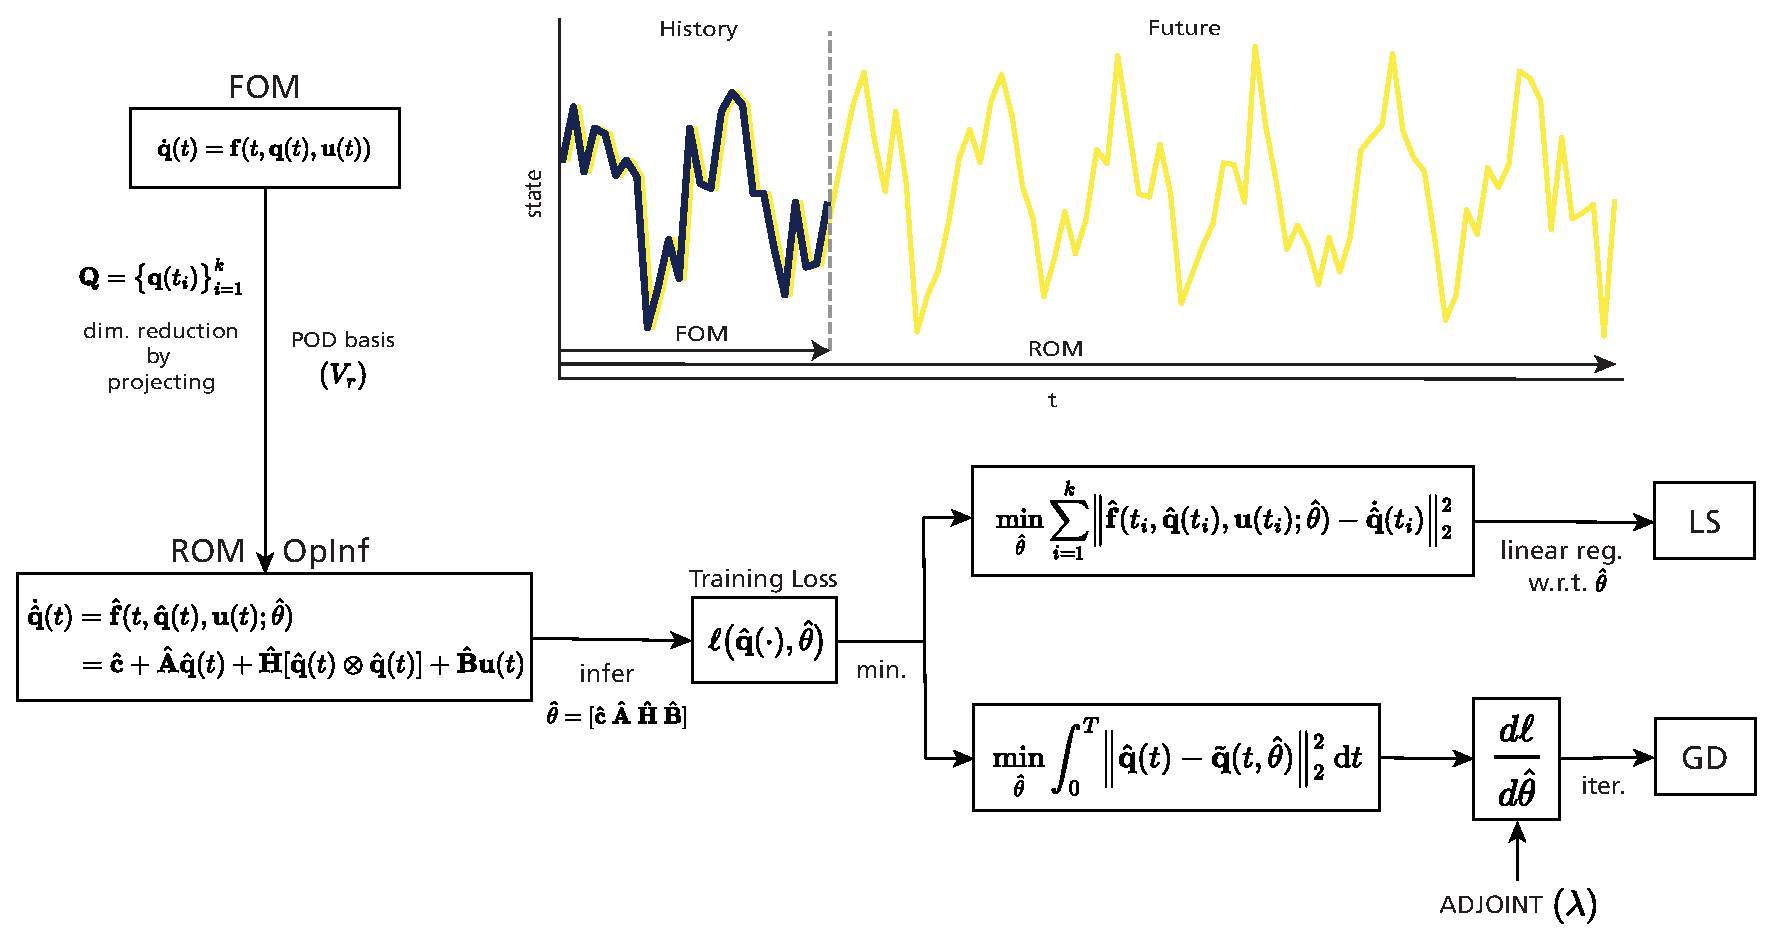
\includegraphics[width=.96\textwidth]{figures/intro_rom.eps}
    \caption{Model Order Reduction and Dual-Branch Minimization in Operator Inference.}
    \label{fig:intro_rom1}
\end{figure}


%%%%%%%%%%%%%%%%%%%%%%%%%%%%%%%%%%%%%%%%%%%%%%%%%%%%%%%%%%%%%%%%%%%%%%%%%%%%%%%%%%%%%%%%%%

\section{The Adjoint-State Equations}
\label{sec:adjoint_eqs}

\subsection*{Problem Setup}

We frame our loss minimization as an equality constraint optimization problem as in \cite{bradley2024pde}, i.e.,\\
\begin{align}
    \underset{\hat{\bm{\theta}} \scalebox{0.67}{$\in$} \hat{\bm{\Theta}}}{\mathrm{min}} ~~&\ell (\hat{\mathbf{q}}(t),\hat{\bm{\theta}})\notag\\
    \mathrm{s.t.}~~&\dot{\hat{\mathbf{q}}}(t) = \hat{\mathbf{f}}(\hat{\mathbf{q}}(t),\hat{\bm{\theta}}), \quad\hat{\mathbf{q}}(0)=\hat{\mathbf{q}}_0, \quad t\in[0,T],
    \label{eq:opt_problem}
\end{align}
where $\ell$ is the loss functional defined as in \eqref{eq:continuous_loss} and the constraint represents the ROM-OpInf as in \eqref{eq:redopinf}.

For such problem, the classical adjoint method as stated in \cite{bradley2024pde,luchini2024introduction} gives the following result.

\begin{theorem}[Adjoint method]
    \label{thm:adjoint_method}
    Assume $\hat{\mathbf{f}}$ and $g$ are continuously differentiable in both $\hat{\mathbf{q}}$ and $\hat{\bm{\theta}}$ and that the initial state $\hat{\mathbf{q}}(0)=\hat{\mathbf{q}}_0$ is fixed (independent of $\hat{\bm{\theta}}$). The adjoint variable $\bm{\lambda}(t)\in\mathcal{C}^1(\mathcal{T})^r$ associated to a minimization problem such in \eqref{eq:opt_problem} satisfies a back propagation ODE\\ 
    \begin{equation}
        \dot{\bm{\lambda}}(t) = -\left[ \left(\dfrac{\partial \hat{\mathbf{f}}}{\partial\hat{\mathbf{q}}}\right)^{\top}\bm{\lambda}(t) + \left( \dfrac{\partial g}{\partial \hat{\mathbf{q}}} \right)^{\top} \right],\quad\bm{\lambda}(T)=0,
        \label{eq:adjoint_eqs}
    \end{equation}
    and the gradients w.r.t. the parameters of the training loss ($\ell$),\\
    \begin{equation*}
        \ell\bigl(\hat{\mathbf{q}}(\cdot),\hat{\bm{\theta}}\bigr) \coloneqq \displaystyle\int_0^T g\bigl(\hat{\mathbf{q}}(t),\hat{\bm{\theta}}\bigr)~\dd t = \int_0^T \norm{\hat{\mathbf{q}}(t) - \tilde{\mathbf{q}}(t, \hat{\bm{\theta}})}_2^2~\dd t
    \end{equation*}
    and the Lagrange cost ($\mathscr{L}$),\\
    \begin{equation*}
        \mathscr{L}\bigl(\hat{\mathbf{q}}(\cdot),\bm{\lambda}(\cdot);\hat{\bm{\theta}}\bigr) \coloneqq \ell\bigl(\hat{\mathbf{q}}(t),\hat{\bm{\theta}}\bigr) - \int_0^T \bm{\lambda}(t)^{\top}\left( \dot{\hat{\mathbf{q}}}(t)-\hat{\mathbf{f}}(\hat{\mathbf{q}}(t),\hat{\bm{\theta}}) \right)\dd t - \bm{\lambda}(0)^{\top}(\hat{\mathbf{q}}(0)-\hat{\mathbf{q}}_0)
        \label{eq:lagrange_cost}
    \end{equation*}
    have the form\\
    \begin{equation}
        \dfrac{\textrm{d} \ell}{\textrm{d} \hat{\bm{\theta}}} = \dfrac{\textrm{d} \mathscr{L}}{\textrm{d}\hat{\bm{\theta}}} = \int_0^T \left(\bm{\lambda}(t)^{\top}\dfrac{\partial\hat{\mathbf{f}}}{\partial\hat{\bm{\theta}}} + \dfrac{\partial g}{\partial\hat{\bm{\theta}}} \right)\dd t.
        \label{eq:gradient_lagrange}
    \end{equation}
\end{theorem}

\subsection*{Proof by Calculus of Variations}

This proof was inspired by the notes of \cite{mcquarrie2024bayesian}. For convenience, we write the constraint equation as\\ 
$$\boldsymbol{c}(\hat{\mathbf{q}}(t),\hat{\bm{\theta}}) \coloneqq \dot{\hat{\mathbf{q}}}(t) - \hat{\mathbf{c}} - \hat{\mathbf{A}}\hat{\mathbf{q}}(t) - \hat{\mathbf{H}}[\hat{\mathbf{q}}(t)\otimes \hat{\mathbf{q}}(t)] - \hat{\mathbf{B}}\mathbf{u}.$$
Here, $\hat{\mathbf{H}}\in \mathbb{R}^{r\times r^2}$ is Kronecker-symmetric, i.e., $\hat{\mathbf{H}}[\hat{\mathbf{q}}\otimes \mathbf{v}] = \hat{\mathbf{H}}[\mathbf{v}\otimes \hat{\mathbf{q}}]$. Then, the Lagrangian (objective - adjoint $\times$ constraint - adjoint(0) $\times$ initial condition) can be rewritten as\\
\begin{align*}
    \mathscr{L}(\hat{\mathbf{q}}, \bm{\lambda}; \hat{\bm{\theta}}) &= \ell(\hat{\mathbf{q}},\hat{\bm{\theta}}) - \int_0^T \bm{\lambda}(t)^{\top}\boldsymbol{c}(\hat{\mathbf{q}}(t),\hat{\bm{\theta}})~\mathrm{d}t - \bm{\lambda}(0)^{\top}(\hat{\mathbf{q}}(0)-\hat{\mathbf{q}}_0)\\
    &= \int_0^T g\bigl(\hat{\mathbf{q}}(t),\hat{\bm{\theta}} \bigl)~\mathrm{d}t \\
    &- \int_0^T \bm{\lambda}(t)^{\top}\bigl(\dot{\hat{\mathbf{q}}}(t) - \hat{\mathbf{c}} - \hat{\mathbf{A}}\hat{\mathbf{q}}(t) - \hat{\mathbf{H}}(\hat{\mathbf{q}}(t)\otimes \hat{\mathbf{q}}(t)) - \hat{\mathbf{B}}\mathbf{u}\bigr)~\mathrm{d}t \\
    &-\bm{\lambda}(0)^{\top}(\hat{\mathbf{q}}(0)-\hat{\mathbf{q}}_0),
\end{align*}
where the adjoint variable $\bm{\lambda}\in\mathcal{C}^1(\mathcal{T})^r$ has the same size as the state variable $\hat{\mathbf{q}}$. The adjoint equation for $\bm{\lambda}(t)$ is derived by setting\\
$$ \bm{D}_{\hat{\mathbf{q}}} \mathscr{L}(\hat{\mathbf{q}},\bm{\lambda,\hat{\bm{\theta}}};\mathbf{v}) = \dv{}{\varepsilon}[\mathscr{L}(\hat{\mathbf{q}}+\varepsilon \mathbf{v},\bm{\lambda,\hat{\bm{\theta}}})]_{\varepsilon=0} = 0~~~\forall~\mathbf{v}\in\mathcal{C}^1(\mathcal{T})^r,~\norm{\mathbf{v}} = 1,$$a directional (Gateaux) derivative \cite{bonnans2013perturbation}. Noting first that\\
\begin{align*}
    \dv{}{\varepsilon}[\mathcal{\ell}(\hat{\mathbf{q}}+\varepsilon \mathbf{v},\hat{\bm{\theta}})]_{\varepsilon=0} &= \int_0^T \dv{}{\varepsilon}[g(\hat{\mathbf{q}}(t)+\varepsilon \mathbf{v}(t),\hat{\bm{\theta}})]_{\varepsilon=0}~\mathrm{d}t = \int_0^T \nabla_{\hat{\mathbf{q}}}~g(\hat{\mathbf{q}}(t),\hat{\bm{\theta}})^{\top}\mathbf{v}(t)~\mathrm{d}t,\\
    \dv{}{\varepsilon}[\boldsymbol{c}(\hat{\mathbf{q}}+\varepsilon \mathbf{v},\hat{\bm{\theta}})]_{\varepsilon=0} &= \dot{\mathbf{v}}(t) - \hat{\mathbf{A}}\mathbf{v}(t) - 2\hat{\mathbf{H}}[\hat{\mathbf{q}}(t)\otimes \mathbf{v}(t)],
\end{align*}
the adjoint equations are given by\\
\begin{align*}
    0 &= \int_0^T \nabla_{\hat{\mathbf{q}}}~g(\hat{\mathbf{q}}(t),\hat{\bm{\theta}})^{\top}\mathbf{v}(t)~\mathrm{d}t\\
    &- \int_0^T \bm{\lambda}(t)^{\top} \left( \dot{\mathbf{v}}(t) - \hat{\mathbf{A}}\mathbf{v}(t) - 2\hat{\mathbf{H}}[\hat{\mathbf{q}}(t)\otimes \mathbf{v}(t)] \right)~\mathrm{d}t~- \bm{\lambda}(0)^{\top}\mathbf{v}(0). 
\end{align*}
We want to write these adjoint equations as a weak form with test function $\mathbf{v}$. Integration by parts yields\\
\begin{align*}
    -\int_0^T\bm{\lambda}(t)^{\top} \dot{\mathbf{v}}(t)~\mathrm{d}t &= -\left[ \bm{\lambda}(t)^{\top} \mathbf{v}(t) \right]_0^T + \int_0^T \dot{\bm{\lambda}}(t)^{\top}\mathbf{v}(t)~\mathrm{d}t\\
    &= \bm{\lambda}(0)^{\top} \mathbf{v}(0) - \bm{\lambda}(T)^{\top} \mathbf{v}(T) + \int_0^T \mathbf{v}(t)^{\top}\dot{\bm{\lambda}}(t)~\mathrm{d}t.
\end{align*}
Using this identity and transposing each (scalar) term, the adjoint equations become\\
\begin{equation*}
    0 = \int_0^T \mathbf{v}(t)^{\top} \left( \dot{\bm{\lambda}}(t) + \hat{\mathbf{A}}^{\top} \bm{\lambda}(t) + 2\tilde{\mathbf{H}}[\hat{\mathbf{q}}(t)\otimes \bm{\lambda}(t)] + \nabla_{\hat{\mathbf{q}}}~g(\hat{\mathbf{q}}(t),\hat{\bm{\theta}}) \right)\mathrm{d}t - \mathbf{v}(T)^{\top}\bm{\lambda}(T), 
\end{equation*}
where $\tilde{\mathbf{H}}\in\mathbb{R}^{r\times r^2}$ is the matrix such that\\
$$\bm{\lambda}^{\top}\hat{\mathbf{H}}[\hat{\mathbf{q}}\otimes \mathbf{v}] = \mathbf{v}^{\top}\tilde{\mathbf{H}}[\hat{\mathbf{q}}\otimes \bm{\lambda}],~~~\forall~\hat{\mathbf{q}}, \mathbf{v}, \bm{\lambda} \in \mathbb{R}^r.$$
Since $\mathbf{v}$ is arbitrary, we recognize the above expression as a weak form with corresponding strong form\\
\begin{equation*}
    -\dot{\bm{\lambda}}(t) = \hat{\mathbf{A}}^{\top} \bm{\lambda}(t) + 2\tilde{\mathbf{H}}[\hat{\mathbf{q}}(t)\otimes \bm{\lambda}(t)] + \nabla_{\hat{\mathbf{q}}}~g(\hat{\mathbf{q}}(t),\hat{\bm{\theta}}),~~~\bm{\lambda}(T)=\bm{0},\quad t\in [0,T].
\end{equation*}
This linear (but non-autonomous) system can be solved with 'backward time-integration' given a trajectory $\hat{\mathbf{q}}(t)$. The system can be written in a more clearly linear form (with respect to $\bm{\lambda}(t)$) as\\
\begin{align*}
     \dot{\bm{\lambda}}(t) &= -\left(\hat{\mathbf{A}}^{\top} + 2\mathbf{M}(\hat{\mathbf{q}}(t))\right)\bm{\lambda}(t) - \nabla_{\hat{\mathbf{q}}}~g(\hat{\mathbf{q}}(t),\hat{\bm{\theta}}),\\
    &~\hspace{8.8cm}~~~~~\bm{\lambda}(T)=\bm{0},\\
    &= -\nabla_{\hat{\mathbf{q}}}~\hat{\mathbf{f}}(\hat{\mathbf{q}}(t),\hat{\bm{\theta}})\bm{\lambda}(t) - \nabla_{\hat{\mathbf{q}}}~g(\hat{\mathbf{q}}(t),\hat{\bm{\theta}}),
\end{align*}
where $\mathbf{M}(\hat{\mathbf{q}}(t))\in\mathbb{R}^{r\times r}$ is the matrix such that\\
\begin{equation*}
    \mathbf{M}(\hat{\mathbf{q}}(t)) \bm{\lambda} = \tilde{\mathbf{H}}[\hat{\mathbf{q}}(t)\otimes \bm{\lambda}(t)].
\end{equation*}
On the other hand, to obtain the derivative of the scalar loss 
$\ell(\hat{\mathbf{q}}(\cdot),\hat{\bm\theta})$ with respect to the parameter~$\hat{\bm\theta}$, 
we note that by construction\\
$$\mathscr L\bigl(\hat q,\lambda;\hat{\bm\theta}\bigr)=\ell - \int_0^T \bm{\lambda}^{\top}(\underbrace{\dot{\hat{\mathbf{q}}} - \hat{\mathbf{f}}}_{= 0,~\forall\hat{\bm{\theta}}\in\hat{\bm{\Theta}}}) ~~~\Rightarrow~~~\dv{\mathscr{L}}{\hat{\bm{\theta}}} = \dv{\ell}{\hat{\bm{\theta}}}.$$
Since in $\mathscr L$ all dependence of $\hat{\mathbf{q}}$ on $\hat{\bm\theta}$ has been
eliminated by the choice of $\bm{\lambda}$, only the explicit partial derivatives remain.  In particular:\\
$$\frac{\mathrm d}{\mathrm d\hat{\bm\theta}}\,
\int_0^T \!g\bigl(\hat{\mathbf{q}}(t),\hat{\bm\theta}\bigr)\,\mathrm d t
=
\int_0^T 
\frac{\partial g}{\partial\hat{\bm\theta}}
\bigl(\hat{\mathbf{q}}(t),\hat{\bm\theta}\bigr)\,
\mathrm d t,$$
and\\
$$\frac{\mathrm d}{\mathrm d\hat{\bm\theta}}\,
\int_0^T \!\bm{\lambda}(t)^\top
\hat{\mathbf{f}}\bigl(\hat{\mathbf{q}}(t),\hat{\bm\theta}\bigr)\,\mathrm d t
=
\int_0^T
\bm{\lambda}(t)^\top\,
\frac{\partial \hat{\mathbf{f}}}{\partial\hat{\bm\theta}}
\bigl(\hat{\mathbf{q}}(t),\hat{\bm\theta}\bigr)\,
\mathrm d t.$$
Thus one arrives at\\
\begin{equation*}
    \dv{}{\hat{\bm{\theta}}}\ell(\hat{\mathbf{q}}(\cdot),\hat{\bm{\theta}}) =  \dv{}{\hat{\bm{\theta}}} \mathscr{L}(\hat{\mathbf{q}},\bm{\lambda},\hat{\bm{\theta}}) = \int_0^T \left(\bm{\lambda}(t)^{\top}\dfrac{\partial\hat{\mathbf{f}}}{\partial\hat{\bm{\theta}}} + \dfrac{\partial g}{\partial\hat{\bm{\theta}}} \right)\dd t.
\end{equation*}
as stated in the theorem.  \qed


\subsection*{Proof by Sensitivity Analysis}

The aim is to obtain the sensitivities $\displaystyle\dv{\ell}{\hat{\bm{\theta}}}$ of a functional of the form\\
$$\ell (\hat{\mathbf{q}},\hat{\bm{\theta}}) = \int_0^T g(\hat{\mathbf{q}}(t),\hat{\bm{\theta}})~\dd t$$
with respect to the parameters $\hat{\bm{\theta}}$, where $g$ represents a quadratic loss of a quantity of interest related to the state $\hat{\mathbf{q}}(t)$ over a certain period of time $t\in[0,T]$. Then, we have\\
$$\dv{\ell}{\hat{\bm{\theta}}} = \int_0^T \dv{\hat{\bm{\theta}}}~g(\hat{\mathbf{q}}(t),\hat{\bm{\theta}})~\dd t = \int_0^T \left(\pdv{g}{\hat{\bm{\theta}}} + \pdv{g}{\hat{\mathbf{q}}} \dv{\hat{\mathbf{q}}}{\hat{\bm{\theta}}} \right)\dd t.$$
In order to avoid the computation of $\displaystyle\dv{\hat{\mathbf{q}}}{\hat{\bm{\theta}}}$, i.e., the sensitity of the trajectory w.r.t. the parameters , which can be extremely hard, we apply a change of variables (adjoint method).

Consider again the following equality constraint minimization problem\\
\begin{align*}
    &\underset{\hat{\bm{\theta}} \scalebox{0.67}{$\in$} \hat{\bm{\Theta}}}{\mathrm{min}} ~~\ell (\hat{\mathbf{q}}(t),\hat{\bm{\theta}})\\
    &\mathrm{s.t.}~~\dot{\hat{\mathbf{q}}}(t) = \hat{\mathbf{f}}(\hat{\mathbf{q}}(t),\hat{\bm{\theta}}),\quad\hat{\mathbf{q}}(t_0)=\hat{\mathbf{q}}_0,
\end{align*}
and a Lagrangian ($\mathscr{L}$) defined as\\
\begin{align*}
    \mathscr{L}(\hat{\mathbf{q}}, \bm{\lambda},\hat{\bm{\theta}}) &\coloneqq \ell(\hat{\mathbf{q}}(t),\hat{\bm{\theta}}) - \int_0^T \bm{\lambda}(t)^{\top}\left( \dot{\hat{\mathbf{q}}}(t) - \hat{\mathbf{f}}(\hat{\mathbf{q}}(t),\hat{\bm{\theta}})  \right)\dd t -\bm{\lambda}(0)^{\top}(\hat{\mathbf{q}}(0)-\hat{\mathbf{q}}_0)\\
    &= \int_0^T \left( g(\hat{\mathbf{q}}(t),\hat{\bm{\theta}}) - \bm{\lambda}(t)^{\top}\left( \dot{\hat{\mathbf{q}}}(t) - \hat{\mathbf{f}}(\hat{\mathbf{q}}(t),\hat{\bm{\theta}})  \right) \right)\dd t-\bm{\lambda}(0)^{\top}(\hat{\mathbf{q}}(0)-\hat{\mathbf{q}}_0).
\end{align*}
Differentiating the Lagrangian w.r.t. $\bm{\theta}$, we have\\
\begin{align*}
    \dv{\mathscr{L}}{\hat{\bm{\theta}}} &= \int_0^T\left[ \pdv{g}{\hat{\bm{\theta}}} + \pdv{g}{\hat{\mathbf{q}}} \dv{\hat{\mathbf{q}}}{\hat{\bm{\theta}}} - \bm{\lambda}(t)^{\top} \left( \dv{t}\dv{\hat{\mathbf{q}}}{\hat{\bm{\theta}}} - \pdv{\hat{\mathbf{f}}}{\hat{\bm{\theta}}} - \pdv{\hat{\mathbf{f}}}{\hat{\mathbf{q}}}\dv{\hat{\mathbf{q}}}{\hat{\bm{\theta}}} \right) \right]\dd t - \bm{\lambda}(0)^{\top}\dv{\hat{\mathbf{q}}}{\hat{\bm{\theta}}}~(0)\notag\\
    &= \int_0^T \left[\pdv{g}{\hat{\bm{\theta}}} + \bm{\lambda}(t)^{\top} \pdv{\hat{\mathbf{f}}}{\hat{\bm{\theta}}}+ \left( \pdv{q}{\hat{\mathbf{q}}} + \bm{\lambda}(t)^{\top}\pdv{\hat{\mathbf{f}}}{\hat{\mathbf{q}}}-\bm{\lambda}(t)^{\top}\dv{t} \right)\dv{\hat{\mathbf{q}}}{\hat{\bm{\theta}}} \right]\dd t- \bm{\lambda}(0)^{\top}\dv{\hat{\mathbf{q}}}{\hat{\bm{\theta}}}~(0). 
\end{align*}
Integrating by parts, we get rid of $\displaystyle\dv{t}\dv{\hat{\mathbf{q}}}{\hat{\bm{\theta}}}$ in the last part of the above integral,\\
\begin{align*}
    \int_0^T -\bm{\lambda}(t)^{\top}\dv{t}\dv{\hat{\mathbf{q}}}{\hat{\bm{\theta}}}~\dd t &= \left[ -\bm{\lambda}(t)^{\top}\dv{\hat{\mathbf{q}}}{\hat{\bm{\theta}}}\right]_0^T + \int_0^T \left( \dv{\bm{\lambda}}{t}\right)^{\top}\dv{\hat{\mathbf{q}}}{\hat{\bm{\theta}}}~\dd t\\
    &= \bm{\lambda}(0)^{\top}\dv{\hat{\mathbf{q}}}{\hat{\bm{\theta}}}~(0) - \bm{\lambda}(T)^{\top}\dv{\hat{\mathbf{q}}}{\hat{\bm{\theta}}}~(T) + \int_0^T \left( \dv{\bm{\lambda}}{t}\right)^{\top}\dv{\hat{\mathbf{q}}}{\hat{\bm{\theta}}}~\dd t.
\end{align*}
Plugin this expression, the Lagrangian sensitivity equation  yields\\
\begin{align*}
   \dv{\mathscr{L}}{\hat{\bm{\theta}}} &= \int_0^T\left[ \pdv{g}{\hat{\bm{\theta}}} + \bm{\lambda}(t)^{\top} \pdv{\hat{\mathbf{f}}}{\hat{\bm{\theta}}} + \underbrace{\left( \pdv{q}{\hat{\mathbf{q}}} + \bm{\lambda}(t)^{\top}\pdv{\hat{\mathbf{f}}}{\hat{\mathbf{q}}}+ \dot{\bm{\lambda}}(t)^{\top}\right)}_{\text{make = 0}} \dv{\hat{\mathbf{q}}}{\hat{\bm{\theta}}} \right]\dd t \\
   & - \bm{\lambda}(0)^{\top}\dv{\hat{\mathbf{q}}}{\hat{\bm{\theta}}}~(0)+\bm{\lambda}(0)^{\top}\dv{\hat{\mathbf{q}}}{\hat{\bm{\theta}}}~(0) - \underbrace{\bm{\lambda}(T)^{\top}\dv{\hat{\mathbf{q}}}{\hat{\bm{\theta}}}~(T)}_{\text{make = 0}}.
\end{align*}
 After transposing and rearranging terms, we obtain the desired adjoint equations\\
\begin{equation*}
    \dot{\bm{\lambda}}(t) = -\left[ \left(\pdv{\hat{\mathbf{f}}}{\hat{\mathbf{q}}}\right)^{\top} \bm{\lambda}(t)  + \left(\pdv{g}{\hat{\mathbf{q}}}\right)^{\top}\right], \quad\bm{\lambda}(T) = \bm{0}.
\end{equation*}

By construction, as we have shown in the first proof,  minimizing the Lagrangian $\mathscr{L}$ is the same as minimizing the loss functional $\ell$ since\\
$$\dv{\mathscr{L}}{\hat{\bm{\theta}}} = \dv{\ell}{\hat{\bm{\theta}}}.$$
Thus, we arrive at the final expression for the gradients, which concludes the proof\\
\begin{equation*}
    \dv{\mathscr{L}}{\hat{\bm{\theta}}} =\dv{\ell}{\hat{\bm{\theta}}} = \int_0^T\left(  \bm{\lambda}(t)^{\top} \pdv{\hat{\mathbf{f}}}{\hat{\bm{\theta}}} + \pdv{g}{\hat{\bm{\theta}}} \right)\dd t .
\end{equation*}
\qed

\subsection*{Theoretical Validation}

One question that arises at this point is whether the solution provided by the adjoint method $\bm{\lambda}(t)$, obtained by solving the backward propagation ODE, is indeed correct and reliable for guiding the optimization of $\hat{\bm{\theta}}$. To address this, we present both theoretical and possible empirical verification arguments in support of the adjoint approach.

The correctness of the adjoint method follows from three fundamental principles of mathematical optimization:

\begin{itemize}
    \item \textbf{Optimality Conditions.}  The adjoint equations emerge directly from the Karush-Kuhn-Tucker (KKT) conditions for constrained optimization \cite{nocedal1999numerical}. By forming the Lagrangian\\
    $$\mathscr{L}(\hat{\mathbf{q}}, \bm{\lambda}, \hat{\bm{\theta}}) 
    = \int_{t_0}^{t_f} g(\hat{\mathbf{q}}(t),\hat{\bm{\theta}}) \,\mathrm{d}t
      - \int_{t_0}^{t_f} \bm{\lambda}(t)^\top \bigl[\dot{\hat{\mathbf{q}}}(t)-\hat{\mathbf{f}}(\hat{\mathbf{q}}(t),\hat{\bm{\theta}})\bigr]\,\mathrm{d}t
      - \bm{\lambda}(t_0)^\top \bigl(\hat{\mathbf{q}}(t_0)-\hat{\mathbf{q}}_0\bigr) ,$$
  the first-order stationarity conditions with respect to~$\hat{\mathbf{q}}$ yield the adjoint ODE that ensures the computed gradients respect the dynamical constraints.
    
    \item \textbf{Duality}: The adjoint variable $\bm{\lambda}(t)$ has a fundamental interpretation as sensitivity measure. Specifically, it quantifies how perturbations in the state vector $\hat{\mathbf{q}}(t)$ propagate through the system to affect the final loss. This duality perspective aligns with reverse-mode automatic differentiation in machine learning \cite{chen2018neural}, where gradients flow backward through computational graphs.

    \item \textbf{Consistency with Pontryagin's Maximum Principle.}  Defining the Hamiltonian\\
  $$\mathcal{H}(\hat{\mathbf{q}}, \bm{\lambda}, \hat{\bm{\theta}}) 
      = \bm{\lambda}^\top \hat{\mathbf{f}}(\hat{\mathbf{q}}, \hat{\bm{\theta}}) 
      + g(\hat{\mathbf{q}}, \hat{\bm{\theta}}),$$
  Pontryagin's principle prescribes the costate equation\\
  $$\dot{\bm{\lambda}}(t) 
      = - \left(\frac{\partial \mathcal{H}}{\partial \hat{\mathbf{q}}} \right)^{\top}
      = - \left(\frac{\partial \hat{\mathbf{f}}}{\partial \hat{\mathbf{q}}} \right)^{\top}\bm{\lambda}(t) -  \left(\frac{\partial g}{\partial \hat{\mathbf{q}}} \right)^{\top}.$$
  The adjoint method exactly recovers these necessary conditions for optimality in control theory \cite{liberzon2011calculus}.
\end{itemize}

In conclusion, the adjoint method computes the costate $\bm{\lambda}(t)$ by rigorously enforcing the first-order optimality conditions of the Lagrangian in a dynamical setting. Its theoretical basis in the Karush-Kuhn-Tucker framework, duality interpretation, and alignment with Pontryagin's principle ensures that the resulting gradients are exact up to numerical precision. Coupled with empirical validation strategies such as finite-difference gradient checking, convergence monitoring, and assessment of physical plausibility, the adjoint method provides a reliable and accurate mechanism for optimizing parameters in dynamical systems.

%%%%%%%%%%%%%%%%%%%%%%%%%%%%%%%%%%%%%%%%%%%%%%%%%%%%%%%%%%%%%%%%%%%%%%%%%%%%%%%%%%%%%%%%

\section{Equations of the Four Gradients}

Note that the adjoint method used here requires computing the following four gradients:\\
$$\pdv{\hat{\mathbf{f}}}{\hat{\mathbf{q}}},  \quad \pdv{g}{\hat{\mathbf{q}}}, \quad \pdv{\hat{\mathbf{f}}}{\hat{\bm{\theta}}},\quad \text{and} \quad \pdv{g}{\hat{\bm{\theta}}},$$
where $\hat{\mathbf{f}}(\hat{\mathbf{q}}, \hat{\bm{\theta}})$ denotes the right-hand side of the reduced-order model (ROM-OpInf) dynamics, and $g(\hat{\mathbf{q}}, \hat{\bm{\theta}})$ is the integrand of the loss functional. The efficient computation of these gradients is crucial for both the backward integration of the adjoint equation and for evaluating the total derivative of the loss function $\ell$. What follows is a detailed derivation of the expressions of each of these gradients.

\subsection{$\bm{\nabla}_{\hat{\mathbf{q}}}~\hat{\mathbf{f}}\bigl(\hat{\mathbf{q}}(t), \hat{\bm{\theta}}\bigr)$}

We begin by recalling the definition:\\
$$
\hat{\mathbf{f}}(\hat{\mathbf{q}}(t), \hat{\bm{\theta}}) = \hat{\mathbf{c}} + \hat{\mathbf{A}}\hat{\mathbf{q}}(t) + \hat{\mathbf{H}}\bigl( \hat{\mathbf{q}}(t)\otimes \hat{\mathbf{q}}(t) \bigr) + \hat{\mathbf{B}}\mathbf{u}(t).
$$
To compute the derivative of $\hat{\mathbf{f}}$ with respect to $\hat{\mathbf{q}}$, we consider the Gâteaux derivative in the direction of an arbitrary vector $\mathbf{v}\in \mathcal{C}^1(\mathcal{T})^r$:\\
$$
\bm{D}_{\hat{\mathbf{q}}}~\hat{\mathbf{f}}(\hat{\mathbf{q}}, \hat{\bm{\theta}}; \mathbf{v}) = \bm{D}_{\hat{\mathbf{q}}}~\hat{\mathbf{f}}[\mathbf{v}] = \lim_{\varepsilon \to 0} \frac{\hat{\mathbf{f}}(\hat{\mathbf{q}} + \varepsilon \mathbf{v}, \hat{\bm{\theta}}) - \hat{\mathbf{f}}(\hat{\mathbf{q}}, \hat{\bm{\theta}})}{\varepsilon} = \dv{}{\varepsilon} \left[ \hat{\mathbf{f}}(\hat{\mathbf{q}} + \varepsilon \mathbf{v}, \hat{\bm{\theta}}) \right]_{\varepsilon = 0}.
$$
Expanding the function $\hat{\mathbf{f}}$ at $\hat{\mathbf{q}} + \varepsilon \mathbf{v}$, we obtain:\\
$$
\hat{\mathbf{f}}(\hat{\mathbf{q}} + \varepsilon \mathbf{v}, \hat{\bm{\theta}}) = \hat{\mathbf{c}} + \hat{\mathbf{A}}(\hat{\mathbf{q}} + \varepsilon \mathbf{v}) + \hat{\mathbf{H}}\bigl( (\hat{\mathbf{q}} + \varepsilon \mathbf{v}) \otimes (\hat{\mathbf{q}} + \varepsilon \mathbf{v}) \bigr) + \hat{\mathbf{B}}\mathbf{u}(t).
$$
The quadratic term expands as:\\
$$
(\hat{\mathbf{q}} + \varepsilon \mathbf{v}) \otimes (\hat{\mathbf{q}} + \varepsilon \mathbf{v}) = \hat{\mathbf{q}} \otimes \hat{\mathbf{q}} + \varepsilon (\hat{\mathbf{q}} \otimes \mathbf{v} + \mathbf{v} \otimes \hat{\mathbf{q}}) + \varepsilon^2 (\mathbf{v} \otimes \mathbf{v}).
$$
Substituting back into the expression for $\hat{\mathbf{f}}$, we get:\\
$$
\hat{\mathbf{f}}(\hat{\mathbf{q}} + \varepsilon \mathbf{v}, \hat{\bm{\theta}}) = \hat{\mathbf{c}} + \hat{\mathbf{A}}\hat{\mathbf{q}} + \varepsilon \hat{\mathbf{A}}\mathbf{v} + \hat{\mathbf{H}}(\hat{\mathbf{q}} \otimes \hat{\mathbf{q}}) + \varepsilon \hat{\mathbf{H}}(\hat{\mathbf{q}} \otimes \mathbf{v} + \mathbf{v} \otimes \hat{\mathbf{q}}) + \hat{\mathbf{B}}\mathbf{u}(t) + \mathcal{O}(\varepsilon^2).
$$
Differentiating with respect to $\varepsilon$ and evaluating at $\varepsilon = 0$ yields:\\
$$
\bm{D}_{\hat{\mathbf{q}}}~\hat{\mathbf{f}}[\mathbf{v}] = \hat{\mathbf{A}}\mathbf{v} + 2\hat{\mathbf{H}}(\hat{\mathbf{q}} \otimes \mathbf{v}),
$$
where we use the fact that $\hat{\mathbf{H}}$ is Kronecker symmetric, i.e., $\hat{\mathbf{H}}(\hat{\mathbf{q}} \otimes \mathbf{v}) = \hat{\mathbf{H}}(\mathbf{v} \otimes \hat{\mathbf{q}})$.
To express this as a gradient under the $L^2$ inner product, we match directional derivatives with inner products:\\
$$
\left( \hat{\mathbf{A}} + 2\hat{\mathbf{H}}\bigl( \hat{\mathbf{q}} \otimes \mathbf{I}_r \bigr) \right) \mathbf{v} = \bm{D}_{\hat{\mathbf{q}}}~\hat{\mathbf{f}}[\mathbf{v}] = \langle \nabla_{\hat{\mathbf{q}}}~\hat{\mathbf{f}},\;\mathbf{v} \rangle = \left( \nabla_{\hat{\mathbf{q}}}~\hat{\mathbf{f}} \right)^{\top}  \mathbf{v},
$$
where $\mathbf{I}_r$ is the identity matrix of size $r$. Therefore, the gradient is given by:\\
\begin{equation}
    \nabla_{\hat{\mathbf{q}}}~\hat{\mathbf{f}}(\hat{\mathbf{q}}, \hat{\bm{\theta}}) = \hat{\mathbf{A}}^{\top} + \left( 2\hat{\mathbf{H}}\bigl( \hat{\mathbf{q}} \otimes \mathbf{I}_r \bigr) \right)^{\top} = \hat{\mathbf{A}}^{\top} + 2\mathbf{M}(\hat{\mathbf{q}}) \quad \in \mathbb{R}^{r \times r},
    \label{eq:gradient_1}
\end{equation}
where we define $\mathbf{M}(\hat{\mathbf{q}}(t)) := \left( \hat{\mathbf{H}}( \hat{\mathbf{q}}(t) \otimes \mathbf{I}_r ) \right)^{\top} \in \mathbb{R}^{r \times r}$.

\subsection{$\bm{\nabla}_{\hat{\mathbf{q}}}\,g\bigl(\hat{\mathbf{q}}(t),\hat{\bm{\theta}}\bigr)$}

By definition, the loss is\\
$$\ell\bigl(\hat{\mathbf{q}}(\cdot),\hat{\bm{\theta}}\bigr)=\int_{0}^{T}g\bigl(\hat{\mathbf{q}}(t),\hat{\bm{\theta}}\bigr)\,\mathrm{d}t,$$
with\\
$$g\bigl(\hat{\mathbf{q}}(t),\hat{\bm{\theta}}\bigr)=\left\|\hat{\mathbf{q}}(t)-\Bigl[\hat{\mathbf{q}}(0)+\int_{0}^{t}\Bigl(\hat{\mathbf{c}}+\hat{\mathbf{A}}\hat{\mathbf{q}}(\tau)+\hat{\mathbf{H}}\bigl(\hat{\mathbf{q}}(\tau)\otimes\hat{\mathbf{q}}(\tau)\bigr)+\hat{\mathbf{B}}\mathbf{u}(\tau)\Bigr)\mathrm{d}\tau\Bigr]
\right\|_{2}^{2}.$$
For convenience, we introduce the residual\\
$$\mathbf{r}(t):=\hat{\mathbf{q}}(t)-\hat{\mathbf{q}}(0)-\int_{0}^{t}\Bigl(\hat{\mathbf{c}}
+\hat{\mathbf{A}}\hat{\mathbf{q}}(\tau)
+\hat{\mathbf{H}}\bigl(\hat{\mathbf{q}}(\tau)\otimes\hat{\mathbf{q}}(\tau)\bigr)
+\hat{\mathbf{B}}\mathbf{u}(\tau)
\Bigr)\mathrm{d}\tau.$$
The Gateaux derivative of $\ell$ in the direction $\mathbf{v}(\cdot)$ is\\
\begin{align*}
\bm{D}_{\hat{\mathbf{q}}}\,\ell[\mathbf{v}]
&=\frac{\mathrm{d}}{\mathrm{d}\varepsilon}
\ell\bigl(\hat{\mathbf{q}}+\varepsilon\mathbf{v},\hat{\bm{\theta}}\bigr)\Big|_{\varepsilon=0}=\int_{0}^{T}
\frac{\mathrm{d}}{\mathrm{d}\varepsilon}g\bigl(\hat{\mathbf{q}}(t)+\varepsilon\mathbf{v}(t),\hat{\bm{\theta}}\bigr)\Big|_{\varepsilon=0}\,\mathrm{d}t\\
&=\int_{0}^{T}\nabla_{\hat{\mathbf{q}}}g\bigl(\hat{\mathbf{q}}(t),\hat{\bm{\theta}}\bigr)^{\!\top}
\mathbf{v}(t)\,\mathrm{d}t.
\end{align*}

Expanding the derivative of $g$, we have\\
\begin{align*}
    &\dv{}{\varepsilon}
     \left\| \hat{\mathbf{q}}(t) + \varepsilon\mathbf{v}(t)
        - \left[
            \hat{\mathbf{q}}(0) + \varepsilon\mathbf{v}(0)
            + \int_0^t \Bigl(
                \hat{\mathbf{c}} 
                + \hat{\mathbf{A}}\hat{\mathbf{q}}(\tau)
                + \varepsilon\hat{\mathbf{A}}\mathbf{v}(\tau) \right. \right. \\
    &
                + \hat{\mathbf{H}}\big(\hat{\mathbf{q}}(\tau) \otimes \hat{\mathbf{q}}(\tau)\big)
                + 2\varepsilon\hat{\mathbf{H}}\big(\hat{\mathbf{q}}(\tau) \otimes \mathbf{v}(\tau)\big)
                + \hat{\mathbf{B}}\mathbf{u}(\tau)
                + \mathcal{O}(\varepsilon^2)
            \Bigr) \dd\tau
        \left. \left. \vphantom{\int_0^t} \right] \right\|_2^2 \Big|_{\varepsilon=0}.
\end{align*}
Rearranging terms,\\
\begin{align*}
&\frac{\mathrm d}{\mathrm d\varepsilon}
 \biggl\|
   \hat{\mathbf{q}}(t)
   - \Bigl[
       \hat{\mathbf{q}}(0)
       + \int_{0}^{t}
           \bigl(
             \hat{\mathbf{c}}
             + \hat{\mathbf{A}}\,\hat{\mathbf{q}}(\tau)
             + \hat{\mathbf{H}}\bigl(\hat{\mathbf{q}}(\tau)\otimes\hat{\mathbf{q}}(\tau)\bigr)
             + \hat{\mathbf{B}}\,\mathbf{u}(\tau)
           \bigr)
         \,\mathrm d\tau
     \Bigr] \\
&\quad\quad
 + \,\varepsilon\,
   \Bigl[
     \mathbf{v}(t)
     - \Bigl(
         \mathbf{v}(0)
         + \int_{0}^{t}
             \bigl(
               \hat{\mathbf{A}}\,\mathbf{v}(\tau)
               + 2\,\hat{\mathbf{H}}\bigl(\hat{\mathbf{q}}(\tau)\otimes\mathbf{v}(\tau)\bigr)
               + \mathcal{O}(\varepsilon)
             \bigr)
           \,\mathrm d\tau
       \Bigr)
   \Bigr]
 \biggr\|_{2}^{2}
 \Big|_{\varepsilon=0}.
\end{align*}
Because $\mathbf{v}$ is arbitrary, we may without loss of generality take $\mathbf{v}(0)=\bm{0}$ and hence the expression simplifies to\\ 
\begin{align*}
&\frac{\mathrm{d}}{\mathrm{d}\varepsilon}\,\Big\|\,\mathbf{r}(t)+ \varepsilon\Bigl[\mathbf{v}(t)- \int_{0}^{t}\bigl(\hat{\mathbf{A}}\mathbf{v}(\tau)+2\,\hat{\mathbf{H}}\bigl(\hat{\mathbf{q}}(\tau)\otimes\mathbf{v}(\tau)\bigr)+ \mathcal{O}(\varepsilon)\big)\,\mathrm{d}\tau\Bigr]\Big\|_{2}^{2}\Big|_{\varepsilon=0}\\
&=2\,\mathbf{r}(t)^{\!\top}\Bigl[\mathbf{v}(t)- \int_{0}^{t}\bigl(\hat{\mathbf{A}}\mathbf{v}(\tau)+2\,\hat{\mathbf{H}}\bigl(\hat{\mathbf{q}}(\tau)\otimes\mathbf{v}(\tau)\bigr)\bigr)\mathrm{d}\tau\Bigr],
\label{eq:Dg_directional}
\end{align*}
where the last equality follows from the identity\\
$$\frac{d}{d\varepsilon}\|\mathbf{r} + \varepsilon\,\mathbf{y}\|^2
= \frac{d}{d\varepsilon}\bigl[(\mathbf{r} + \varepsilon\,\mathbf{y})^\top (\mathbf{r} + \varepsilon\,\mathbf{y})\bigr]= 2\,(\mathbf{r} + \varepsilon\,\mathbf{y})^\top\,\mathbf{y}.$$
Hence,\\
\begin{align*}
\bm{D}_{\hat{\mathbf{q}}}\,\ell[\mathbf{v}]&=2\int_{0}^{T}\mathbf{r}(t)^{\!\top}\mathbf{v}(t)\,\mathrm{d}t
-2\int_{0}^{T}\mathbf{r}(t)^{\!\top}\int_{0}^{t}\hat{\mathbf{A}}\mathbf{v}(\tau)\,\mathrm{d}\tau\,\mathrm{d}t\\
&-4\int_{0}^{T}\mathbf{r}(t)^{\!\top}\int_{0}^{t}\hat{\mathbf{H}}\bigl(\hat{\mathbf{q}}(\tau)\otimes\mathbf{v}(\tau)\bigr)\,\mathrm{d}\tau\,\mathrm{d}t.
\end{align*}
By Fubini’s theorem we swap integrals\\
\begin{align*}
\bm{D}_{\hat{\mathbf{q}}}\,\ell[\mathbf{v}]&=2\int_{0}^{T}\mathbf{r}(\tau)^{\!\top}\mathbf{v}(\tau)\,\mathrm{d}\tau-2\int_{0}^{T}\Bigl[\int_{\tau}^{T}\mathbf{r}(t)^{\!\top}\hat{\mathbf{A}}\,\mathrm{d}t\Bigr]\mathbf{v}(\tau)\,\mathrm{d}\tau\\
&\quad-4\int_{0}^{T}\Bigl[\int_{\tau}^{T}\mathbf{r}(t)^{\!\top}\,\hat{\mathbf{H}}\bigl(\hat{\mathbf{q}}(\tau)\otimes\mathbf{I}_r\bigr)\,\mathrm{d}t\Bigr]\mathbf{v}(\tau)\,\mathrm{d}\tau.
\end{align*}
Thus, comparing with the inner-product form\\
$$\bm{D}_{\hat{\mathbf{q}}}\,\ell[\mathbf{v}]=\int_{0}^{T}\bigl(\nabla_{\hat{\mathbf{q}}}\,g\bigr)^{\!\top}\mathbf{v}\,\mathrm{d}t,$$
we read off the expression for the final gradient\\
\begin{equation}
\label{eq:gradient_3}
\nabla_{\hat{\mathbf{q}}}\,g\bigl(\hat{\mathbf{q}}(t),\hat{\bm{\theta}}\bigr)
=2\,\mathbf{r}(t)-2\,\hat{\mathbf{A}}^{\!\top}\int_{t}^{T}\mathbf{r}(\tau)\,\mathrm{d}\tau
-4\,\mathbf{M}(\hat{\mathbf{q}}(t))\int_{t}^{T}\mathbf{r}(\tau)\,\mathrm{d}\tau \quad\in\mathbb{R}^{r},
\end{equation}
where
$$\mathbf{M}(\hat{\mathbf{q}}(t)):=\Bigl(\hat{\mathbf{H}}\bigl(\hat{\mathbf{q}}(t)\otimes\mathbf{I}_r\bigr)\Bigr)^{\!\top}.$$

\subsection{$\bm{\nabla}_{\hat{\bm{\theta}}}\,\hat{\mathbf{f}}\bigl(\hat{\mathbf{q}}(t),\,\hat{\bm{\theta}}\bigr)$}

Recall that, according to Definition \ref{def:continuous_loss}, the parameter vector is defined as\\
$$\hat{\bm{\theta}}=\bigl[\,\underbrace{\hat{\mathbf{c}}}_{\in\mathbb{R}^r}\;,\;\underbrace{\operatorname{vec}(\hat{\mathbf{A}})}_{\in\mathbb{R}^{r^2}}\;,\;\underbrace{\operatorname{vec}(\hat{\mathbf{H}})}_{\in\mathbb{R}^{r^3}}\;,\;\underbrace{\operatorname{vec}(\hat{\mathbf{B}})}_{\in\mathbb{R}^{rm}}\bigr]\;\in\; \mathbb{R}^d,\quad d = r + r^2 + r^3 + rm.$$
In order to compute each block independently, we split the gradient into four sub-blocks\\
$$\nabla_{\hat{\bm{\theta}}}\,\hat{\mathbf{f}} = \begin{bmatrix}
\nabla_{\hat{\mathbf{c}}}\,\hat{\mathbf{f}} \\
\nabla_{\hat{\mathbf{A}}}\,\hat{\mathbf{f}} \\
\nabla_{\hat{\mathbf{H}}}\,\hat{\mathbf{f}} \\
\nabla_{\hat{\mathbf{B}}}\,\hat{\mathbf{f}} 
\end{bmatrix}:$$
\noindent\textbf{(i)} Gradient w.r.t. $\hat{\mathbf{c}}$.

For any direction \(\mathbf{v}_{\hat{\mathbf{c}}}\in\mathbb{R}^r\),\\
$$\bm{D}_{\hat{\mathbf{c}}}~\hat{\mathbf{f}}[\mathbf{v}_{\hat{\mathbf{c}}}] = \dv{}{\varepsilon}\Bigl(\hat{\mathbf{c}}+\varepsilon\,\mathbf{v}_{\hat{\mathbf{c}}}\Bigr)\Big|_{\varepsilon=0} = \mathbf{v}_{\hat{\mathbf{c}}}\;=\;\langle \mathbf{I}_r,\;\mathbf{v}_{\hat{\mathbf{c}}}\rangle = \bigl(\nabla_{\hat{\mathbf{c}}}\hat{\mathbf{f}}\bigr)^{\!\top}\!\mathbf{v}_{\hat{\mathbf{c}}},$$
so\\
$$\nabla_{\hat{\mathbf{c}}}\,\hat{\mathbf{f}}=\mathbf{I}_r\;\in\;\mathbb{R}^{r\times r}.$$
\noindent\textbf{(ii)} Gradient w.r.t. $\hat{\mathbf{A}}$.

For any $\mathbf{V}_A\in\mathbb{R}^{r\times r}$ with $\tilde{\mathbf{v}}_A=\operatorname{vec}(\mathbf{V}_A)\in\mathbb{R}^{r^2}$,\\
$$\bm{D}_{\hat{\mathbf{A}}}~\hat{\mathbf{f}}[\mathbf{V}_A] = \dv{}{\varepsilon}\Bigl((\hat{\mathbf{A}}+\varepsilon\mathbf{V}_A)\,\hat{\mathbf{q}}\Bigr)\Big|_{\varepsilon=0}=\mathbf{V}_A\,\hat{\mathbf{q}}=\langle\hat{\mathbf{q}}^{\top}\otimes\mathbf{I}_r,\;\tilde{\mathbf{v}}_A\rangle=\bigl(\nabla_{\hat{\mathbf{A}}}\hat{\mathbf{f}}\bigr)^{\!\top}\!\tilde{\mathbf{v}}_A,$$
hence\\
$$\nabla_{\hat{\mathbf{A}}}\,\hat{\mathbf{f}}=\hat{\mathbf{q}}\otimes\mathbf{I}_r\;\in\;\mathbb{R}^{r^2\times r}.$$
\noindent\textbf{(iii)} Gradient w.r.t. $\hat{\mathbf{H}}$.

For any $\mathbf{V}_H\in\mathbb{R}^{r\times r^2}$ with $\tilde{\mathbf{v}}_H=\operatorname{vec}(\mathbf{V}_H)\in\mathbb{R}^{r^3}$,\\
$$\bm{D}_{\hat{\mathbf{H}}}~\hat{\mathbf{f}}[\mathbf{V}_H]=\dv{}{\varepsilon}\Bigl((\hat{\mathbf{H}}+\varepsilon\mathbf{V}_H)\,(\hat{\mathbf{q}}\otimes\hat{\mathbf{q}})\Bigr)\Big|_{\varepsilon=0}=\mathbf{V}_H\,(\hat{\mathbf{q}}\otimes\hat{\mathbf{q}})=\langle(\hat{\mathbf{q}}\otimes\hat{\mathbf{q}})^{\top}\otimes\mathbf{I}_r,\;\tilde{\mathbf{v}}_H\rangle=\bigl(\nabla_{\hat{\mathbf{H}}}\hat{\mathbf{f}}\bigr)^{\!\top}\!\tilde{\mathbf{v}}_H,$$
so\\
$$\nabla_{\hat{\mathbf{H}}}\,\hat{\mathbf{f}}=(\,\hat{\mathbf{q}}\otimes\hat{\mathbf{q}}\,)\otimes\mathbf{I}_r\;\in\;\mathbb{R}^{r^3\times r}.$$
\noindent\textbf{(iv)} Gradient w.r.t. $\hat{\mathbf{B}}$.

Analogously, one shows\\
$$\nabla_{\hat{\mathbf{B}}}\,\hat{\mathbf{f}}=\mathbf{u}(t)\otimes\mathbf{I}_r\;\in\;\mathbb{R}^{rm\times r}.$$
By convenience for a further implementation, we express the gradients w.r.t. $\hat{\bm{\theta}}$ in its transposed form to match the adjoint-method formulation of the loss functional in \eqref{eq:gradient_lagrange}.
Thus, collecting all four transposed blocks, the expression for the gradient yields\\
\begin{equation}
  \label{eq:gradient_2}
  \nabla_{\hat{\bm{\theta}}}^{\top}\,\hat{\mathbf{f}}=\bigl[\,\mathbf{I}_r,\;\hat{\mathbf{q}}(t)^{\!\top}\otimes\mathbf{I}_r,\;(\hat{\mathbf{q}}(t)\otimes\hat{\mathbf{q}}(t))^{\!\top}\otimes\mathbf{I}_r,\;\mathbf{u}(t)^{\!\top}\otimes\mathbf{I}_r\bigr]\;\in\;\mathbb{R}^{r\times d}.
\end{equation}


\subsection{$\bm{\nabla}_{\hat{\bm{\theta}}}~g\bigl(\hat{\mathbf{q}}(t), \hat{\bm{\theta}}\bigr)$}

We recall the pointwise loss integrand,\\
$$g(\hat{\mathbf{q}}(t),\hat{\bm{\theta}}) = \norm{\hat{\mathbf{q}}(t) -\hat{\mathbf{q}}(0) - \int_0^t \bigl[ \hat{\mathbf{c}} + \hat{\mathbf{A}}\hat{\mathbf{q}}(\tau) + \hat{\mathbf{H}}\bigl( \hat{\mathbf{q}}(\tau) \otimes \hat{\mathbf{q}}(\tau) \bigr) + \hat{\mathbf{B}}\mathbf{u}(\tau) \bigr]\dd\tau }_2^2.$$
Similarly to the computation of the gradient of $\hat{\mathbf{f}}$, we consider a perturbation $\hat{\bm{\theta}} + \varepsilon\tilde{\mathbf{v}}$, such that $\tilde{\mathbf{v}}=\operatorname{vec}(\mathbf{V})\in\mathbb{R}^d$ with $\mathbf{V}=[\mathbf{v}_{\hat{\mathbf{c}}}~\mathbf{V}_{\hat{\mathbf{A}}}~\mathbf{V}_{\hat{\mathbf{H}}}~\mathbf{V}_{\hat{\mathbf{B}}}]$ defined as in the previous derivation. Then, we compute\\
\begin{align*}
    \bm{D}_{\hat{\bm{\theta}}}~g[\mathbf{V}] &=\dv{}{\varepsilon}
     \left\| \hat{\mathbf{q}}(t) - \hat{\mathbf{q}}(0) - 
             \int_0^t \Bigl(
                \hat{\mathbf{c}}  + \varepsilon\mathbf{v}_{\hat{c}}
                + \bigl(\hat{\mathbf{A}} + \varepsilon\mathbf{V}_{\hat{\mathbf{A}}}\bigr)\hat{\mathbf{q}}(\tau)
                 \right.  \\
    &
                + \bigl(\hat{\mathbf{H}} + \varepsilon\mathbf{V}_{\hat{\mathbf{H}}}\bigr)
                \bigl(\hat{\mathbf{q}}(\tau) \otimes \hat{\mathbf{q}}(\tau)\bigr)
                + \bigl(\hat{\mathbf{B}} + \varepsilon\mathbf{V}_{\hat{\mathbf{B}}} \bigr)\mathbf{u}(\tau)
            \Bigr) \dd\tau
        \left. \vphantom{\int_0^t}  \right\|_2^2 \Big|_{\varepsilon=0},
\end{align*}
which can be rewritten as\\
\begin{align*}
&\frac{\mathrm{d}}{\mathrm{d}\varepsilon}\,\left\|\,\mathbf{r}(t) - \varepsilon\biggl[ \int_{0}^{t}\bigl(\mathbf{v}_{\hat{\mathbf{c}}} + \mathbf{V}_{\hat{\mathbf{A}}}\hat{\mathbf{q}}(\tau)+\mathbf{V}_{\hat{\mathbf{H}}}\bigl(\hat{\mathbf{q}}(\tau)\otimes\mathbf{v}(\tau)\bigr)+ \mathbf{V}_{\hat{\mathbf{B}}}\mathbf{u}(\tau)\big)\,\mathrm{d}\tau\biggr]\right\|_{2}^{2}\Big|_{\varepsilon=0}\\
&=-2\,\mathbf{r}(t)^{\!\top}\int_{0}^{t}\bigl(\mathbf{v}_{\hat{\mathbf{c}}} + \mathbf{V}_{\hat{\mathbf{A}}}\hat{\mathbf{q}}(\tau)+\mathbf{V}_{\hat{\mathbf{H}}}\bigl(\hat{\mathbf{q}}(\tau)\otimes\mathbf{v}(\tau)\bigr)+ \mathbf{V}_{\hat{\mathbf{B}}}\mathbf{u}(\tau)\big)\,\mathrm{d}\tau.
\end{align*}
We recognize the integrand of the last equality as the first order variation of the function $\hat{\mathbf{f}}$ w.r.t. $\hat{\bm{\theta}}$, hence\\
$$\langle-2\,\mathbf{r}(t)^{\!\top}\int_{0}^{t}\bigl[\,\mathbf{I}_r,\;\hat{\mathbf{q}}(\tau)^{\!\top}\otimes\mathbf{I}_r,\;(\hat{\mathbf{q}}(\tau)\otimes\hat{\mathbf{q}}(\tau))^{\!\top}\otimes\mathbf{I}_r,\;\mathbf{u}(\tau)^{\!\top}\otimes\mathbf{I}_r\bigr]\mathrm{d}\tau,~\tilde{\mathbf{v}}\rangle.$$
Thus, the final (transposed) expression for the gradient yields\\
\begin{equation}
    \nabla_{\hat{\bm{\theta}}}^{\top}~g = -2\int_{0}^{t} \mathbf{r}(\tau)^{\!\top}\bigl[\,\mathbf{I}_r,\;\hat{\mathbf{q}}(\tau)^{\!\top}\otimes\mathbf{I}_r,\;(\hat{\mathbf{q}}(\tau)\otimes\hat{\mathbf{q}}(\tau))^{\!\top}\otimes\mathbf{I}_r,\;\mathbf{u}(\tau)^{\!\top}\otimes\mathbf{I}_r\bigr]\mathrm{d}\tau \quad\in\mathbb{R}^{1\times d}.
    \label{eq:gradient_4}
\end{equation}


%%%%%%%%%%%%%%%%%%%%%%%%%%%%%%%%%%%%%%%%%%%%%%%%%%%%%%%%%%%%%%%%%%%%%%%%%%%%%%%%%%%%%%%%
\section{Gradient Descent for Parameter Optimization}
\label{sec:gd_opt}

Having obtained the gradient of the loss functional $\ell(\hat{\mathbf{q}}(t),\hat{\bm\theta})$ via the adjoint method, we proceed to minimize $\ell$ over $\hat{\bm\theta}\in\hat{\bm{\Theta}}$ using the gradient descent (GD) algorithm \cite{ruder2017overviewgradientdescentoptimization,SENGUPTA2014521}.  Concretely, starting from an initial parameter vector $\hat{\bm\theta}^0$, we generate a sequence $\{\hat{\bm\theta}^j\}_{j\ge0}$ by iteratively stepping against the gradient:\\
\begin{equation}
    \hat{\bm\theta}^{j+1}
    = \hat{\bm\theta}^j
    - \eta_j \,\nabla \ell\bigl(\hat{\mathbf{q}},\hat{\bm\theta}^j\bigr),
    \quad j = 0,1,2,\dots
    \label{eq:gd_update}
\end{equation}
where
\begin{itemize}
  \item $\nabla \ell\bigl(\hat{\mathbf{q}},\hat{\bm\theta}^j\bigr)$ is the gradient computed via the adjoint equations,
  \item $\eta_j>0$ is the step size (learning rate) at iteration~$j$.
\end{itemize}
The procedure halts once a suitable stopping criterion is met. A common stopping condition is\\
\begin{equation}
    \|\nabla \ell\bigl(\hat{\mathbf{q}},\hat{\bm\theta}^j\bigr)\|\;\le\;\epsilon,
    \label{eq:gd_stop}
\end{equation}
for a prescribed tolerance $\epsilon>0$.  Under mild assumptions on~$\ell$ and a proper choice of $\{\eta_j\}$, the iterates $\hat{\bm\theta}^j$ converge to a stationary point of~$\ell$.

\subsection*{Learning rate-Step Size selection and convergence considerations}

The choice of $ \eta_j $ affects the convergence behavior. A constant step size $ \eta_j = \eta $ is commonly used but requires tuning to balance convergence speed and stability.

We introduce two key definitions that will be used in the convergence analysis of the gradient descent method \cite{garrigos2023handbook}.

\begin{definition}[$L$-smooth function]
A differentiable function $\ell: \mathbb{R}^p \to \mathbb{R}$ is said to be $L$-smooth if there exists a constant $L > 0$ such that for all $\bm\omega, \bm{\tilde{\omega}} \in \mathbb{R}^p$,\\
\begin{equation} \label{eq:L_smoothness}
    \| \nabla \ell(\bm{\omega}) - \nabla \ell(\bm{\tilde{\omega}}) \| \leq L \| \bm{\omega} - \bm{\tilde{\omega}} \|.
\end{equation}
This condition ensures that the gradient of $\ell$ is Lipschitz continuous with constant $L$.
\end{definition}

\begin{definition}[$\mu$-strongly convex function]
A function $\ell: \mathbb{R}^p \to \mathbb{R}$ is said to be $\mu$-strongly convex if there exists a constant $\mu > 0$ such that for all $\bm\omega, \bm{\tilde{\omega}} \in \mathbb{R}^p$,\\
\begin{equation} \label{eq:mu_strong_convexity}
    \ell(\bm{\tilde{\omega}}) \geq \ell(\bm\omega) + \nabla \ell(\bm\omega)^{\top}(\bm{\tilde{\omega}} - \bm\omega) + \frac{\mu}{2} \| \bm{\tilde{\omega}} - \bm\omega \|^2.
\end{equation}
\end{definition}
This condition implies that $\ell$ has a lower bound on its curvature, ensuring strong convexity. An equivalent characterization of $\mu$-strong convexity is given in terms of the Hessian matrix:\\
\begin{equation} \label{eq:hessian_characterization}
    \ell ~~ \mu\text{-strongly convex~} \Leftrightarrow \nabla^2 \ell(\bm\omega) \succeq \mu \mathbf{I}, \quad \forall \bm\omega \in \mathbb{R}^p
\end{equation}
where $\nabla^2 \ell(\bm\omega)$ denotes the Hessian of $\ell$ at $\bm\omega$, and $\mu \mathbf{I}$ represents the identity matrix scaled by $\mu$. This ensures that all eigenvalues of the Hessian are at least $\mu$, guaranteeing a strong convexity lower bound.

Under suitable conditions, such as $L$-smoothness and $\mu$-strong convexity of $\ell(\bm\omega)$, and an appropriate step size, GD is guaranteed to converge to a minimizer of $\ell(\bm\omega)$ \cite{garrigos2023handbook}. Table \ref{tab:table-01} summarizes the convergence error rates of GD under different smoothness and convexity assumptions for different step-size choices.

\begin{table}[!htpb]
    \centering
    \begin{tabular}{lcc}
        \toprule
        \textbf{Condition} & \textbf{Step Size ($\bm\eta$)} & \textbf{Error Rate} \\ 
        \midrule
        $\ell$ is $L$-smooth  & $\dfrac{1}{L}$  & $\ell(\bm\omega^{j}) - \ell(\bm\omega^{*}) \le \dfrac{1}{j\eta}\norm{\bm\omega^0 - \bm\omega^*}^2$  \\
        \midrule
        \makecell{$\ell$ is $L$-smooth and\\$\mu$-strongly convex}   & $\dfrac{1}{L}$ & $\norm{\bm\omega^{j} - \bm\omega^{*}} \le \left(1-\dfrac{\mu}{L}\right)^j\norm{\bm\omega^0 - \bm\omega^*}$  \\
        \midrule
        \makecell{$\ell$ is $L$-smooth and\\$\mu$-strongly convex}   & $\dfrac{2}{L+\mu}$   & $\norm{\bm\omega^{j} - \bm\omega^{*}} \le \left(\dfrac{L-\mu}{L+\mu}\right)^j\norm{\bm\omega^0 - \bm\omega^*}$  \\
        [1.5em]
        \multicolumn{3}{l}{\textit{Note that $\dfrac{L-\mu}{L+\mu}=\dfrac{\kappa-1}{\kappa+1}$, where $\kappa\coloneqq\dfrac{L}{\mu}$ is the condition number of $~\nabla^2\ell$}} \\
        \bottomrule
    \end{tabular}
    \caption{GD error rates under different smoothness and convexity assumptions.}
    \label{tab:table-01}
\end{table}

For $\mu$-strongly convex $\ell$, two key properties ensure favorable optimization behavior:
\begin{itemize}
    \item Uniqueness of the minimizer, ensuring a well-defined optimization solution.
    \item Fast convergence, with at least linear convergence and exponential error decay. 
\end{itemize}

These properties become particularly relevant in Operator Inference frameworks when an $L^2$-regularization term is added to the loss.  The regularizer enforces strong convexity and smoothness, thus ensuring the above convergence properties.

\newpage

\subsection*{Adaptive Step-Size: Armijo Line Search.} 
Rather than fixing $\eta_j$, Algorithm \ref{algorithm_1} employs a backtracking procedure to adaptively choose $\eta_j$ so that the Armijo sufficient decrease condition is satisfied \cite{nocedal1999numerical}:

\begin{center}
\begin{minipage}{0.95\textwidth}
\begin{algorithm}[H]
\label{algorithm_1}
\SetAlgoLined
\caption{Armijo Backtracking Line Search + Gradient Descent}
\textbf{Step 1. Initialization:} Choose $\alpha\in(0,1)$, $\beta\in(0,1)$, and initial step size $\eta_{0} > 0$. Set iteration counter $j=0$\;
\textbf{Step 2. Compute descent direction:} Evaluate gradient $\mathscr{G}^j = \nabla \ell(\hat{\mathbf{q}},\hat{\bm\theta}^j)$\;
\textbf{Step 3. Backtracking loop:}

$$\eta \;\leftarrow\;\eta_{0}
    \quad\text{while}\quad
    \ell\bigl(\hat{\mathbf{q}},\hat{\bm\theta}^j - \eta\,\mathscr{G}^j\bigr)
    >
    \ell(\hat{\mathbf{q}},\hat{\bm\theta}^j)
    \;-\;\alpha\,\eta\,\|\mathscr{G}^j\|^2
    \quad\text{do}\quad
    \eta \leftarrow \beta\,\eta$$
\textbf{Step 4. Update:} Set step size $\eta_j = \eta$ and update

$$\hat{\bm\theta}^{j+1} = \hat{\bm\theta}^j - \eta_j\,\mathscr{G}^j\,.$$
\textbf{Step 5. Stopping criterion:} If $\|\mathscr{G}^{j+1}\|\le\epsilon$ (or another criterion) then stop; otherwise set $j\leftarrow j+1$ and go to Step 2.
\end{algorithm}
\end{minipage}
\end{center}


In non-convex scenarios, GD may only reach stationary points.  For large-scale or stochastic settings, variants such as Stochastic Gradient Descent (SGD) are often preferred \cite{ruder2017overviewgradientdescentoptimization}.


%%%%%%%%%%%%%%%%%%%%%%%%%%%%%%%%%%%%%%%%%%%%%%%%%%%%%%%%%%%%%%%%%%%%%%%%%%%%%%%%%%%%%%%%

\section{Adjoint Method Algorithm}

Down below, we present a complete adjoint-based training algorithm that integrates data preprocessing, reduced-order modeling, and gradient-based parameter refinement. Algorithm~\ref{algorithm_2} summarizes the workflow: after collecting and optionally preprocessing the full-order data, we obtain an initial parameter guess via Operator Inference, then iteratively solve the forward and adjoint equations to compute gradients and perform backtracking gradient descent until convergence.

%% Final Adjoint Method Algorithm
\begin{center}
\begin{minipage}{0.95\textwidth}
\begin{algorithm}[H]
\caption{Adjoint Method for Parameter Training}\label{algorithm_2}
\SetAlgoNoLine
\textbf{Input:} Full-order snapshots $\mathbf{Q},\mathbf{U}$; backtracking params $(\alpha,\beta,\eta_0)$; tolerance $\epsilon$; training time interval $[t_1, t_k]$; maximum number of iterations $j_{max}$\;
\textbf{Output:} Optimized ROM parameters $\hat{\bm\theta}^*$\;
\vspace{0.3cm}
\textbf{Step 1. Data collection and preprocessing:} Gather snapshots $\mathbf{Q}=[\mathbf{q}_{t_1},\dots,\mathbf{q}_{t_k}]$, $\mathbf{U}=[\mathbf{u}_{t_1},\dots,\mathbf{u}_{t_k}]$.
\quad [Optional] lift/scale/center the data\;
\textbf{Step 2. Dimensionality reduction:} Compute POD basis $\mathbf{V}_r$ (cumulative energy criterion or fixed ROM dimension $r$). Project: $\hat{\mathbf{Q}} \approx \mathbf{V}_r^\top\mathbf{Q}$\;
\textbf{Step 3. Initial parameter guess:} Solve OpInf regression with $\dot{\mathbf{Q}}$ to obtain $\hat{\bm\theta}^{0}_{\text{OpInf}}$\;
\textbf{Step 4. Gradient descent loop:}
Initialize $j=0$, $\hat{\bm\theta}^j=\hat{\bm\theta}^{0}_{\text{OpInf}}$, and step-size bounds.
\begin{enumerate}[label=\arabic*.]
  \item \textbf{Forward solve:}
    compute ROM solution $\tilde{\mathbf{q}}(t;\hat{\bm\theta}^j)$ via reduced ODE.
  \item \textbf{Residual:}
    set $\mathbf{r}(t)\coloneqq\hat{\mathbf{q}}_{\text{true}}(t)-\tilde{\mathbf{q}}_{\text{pred}}(t;\hat{\bm\theta}^j)$.
  \item \textbf{Adjoint solve:}
    integrate adjoint ODE \eqref{eq:adjoint_eqs} backward for $\bm\lambda(t)$ using Eqs.~\eqref{eq:gradient_1},~\eqref{eq:gradient_3}.
  \item \textbf{Gradient assembly:}
    form $\nabla\ell(\hat{\bm\theta}^j)$ via Eq.~\eqref{eq:gradient_lagrange} using gradients from \eqref{eq:gradient_2},~\eqref{eq:gradient_4}.
  \item \textbf{Armijo line search:}
    choose step size \(\eta_j\) by backtracking (Algorithm~\ref{algorithm_1}).
  \item \textbf{Update:}
    $\hat{\bm\theta}^{j+1}=\hat{\bm\theta}^j-\eta_j\nabla\ell(\hat{\bm\theta}^j)$.
  \item \textbf{Stopping criteria:}
    check convergence, if $\|\nabla\ell(\hat{\bm\theta}^{j+1})\|\le\epsilon$ or $j=j_{max}$, stop; else $j\leftarrow j+1$ and repeat.
\end{enumerate}
\textbf{Step 5. Return} {$\hat{\bm\theta}^*$}.
\end{algorithm}
\end{minipage}
\end{center}
    

%%%%%%%%%%%%%%%%%%%%%%%%%%%%%%%%%%%%%%%%%%%%%%
%%%%%%%%%%%%%%%%%%%%%%%%%%%%%%%%%%%%%%%%%%%%%%
%%%%%%%%%%%%%%%%%%%%%%%%%%%%%%%%%%%%%%%%%%%%%%




%%%%%%%%%%%%%%%%%%%%%%%%%%%%%%%%%%%%%%%%%%%%%%
%%%%%%%%%%%%%%%%%% EXAMPLES %%%%%%%%%%%%%%%%%%
%%%%%%%%%%%%%%%%%%%%%%%%%%%%%%%%%%%%%%%%%%%%%%

%\begin{theorem}
%Let $ A $ be an $ n \times n $ matrix. If $ A $ is %invertible, then its inverse is unique.
%\end{theorem}

%\begin{proof}
%Suppose there exist two inverses $ B $ and $ C $ such that $ AB = I $ and $ AC = I $. Then,
%\[
%B = BI = B(AC) = (BA)C = IC = C.
%\]
%Thus, the inverse is unique.
%\end{proof}

%\begin{highlightedParagraphC}
 
%The choice of other matrix functions or different types of dynamic walks in the resolvent (\ref{eqn:katz3}), arises a slightly different system of equations.

%\end{highlightedParagraphC}

%\begin{equation}
%\label{eqn:remarks2}
%    \mathbf{U^{\prime}}(t) = -\beta (\mathbf{U}(t) - \mathbf{I}) + \mathbf{U}(t)\log (H(\mathbf{A}(t)))
%\end{equation}

%\begin{definition}
%    A dynamic walk of length $w$ from node $i_1$ to node $i_{w+1}$ consists of a sequence of edges $(i_1,i_2,\dots,i_{w+1})$ and a non-decreasing sequence of times $t_{r_1}\le t_{r_2}\le \cdots \le t_{r_w}$ such that $\mathbf{A}(t_{r_m})_{i_m,i_{m+1}}\ne 0$ for $m=1,2,\dots,w$. The lifetime of a dynamic walk is defined by $t_{r_w} - t_{r_1}$. 
%\end{definition}










  % ADJOINT DERIVATION
	
	\chapter{Numerical Experiments}
\label{chap:numexp}

In this chapter, we evaluate the proposed adjoint-based training method on two canonical nonlinear PDEs: the 1D viscous Burgers’ equation and the 2D Fisher-KPP equation. These test cases were chosen to challenge the reduced-order modeling framework in distinct ways: Burgers’ equation with a small viscosity parameter $\nu=0.01$ produces sharp gradients and nonlinear advection-diffusion interactions, while the Fisher-KPP equation exhibits reaction-diffusion dynamics in two spatial dimensions.  

For each model, we compare the adjoint method against the classical OpInf approach under two perturbation scenarios:
\begin{enumerate}[label=(\roman*)]
  \item reducing the temporal sampling density of the training snapshots, and
  \item adding synthetic noise to the data.
\end{enumerate}
We hypothesize that, because the adjoint method computes exact gradients of the loss functional, it will provide more robust and accurate parameter estimates, especially when training data are noisy or sparsely sampled, than OpInf, which relies on finite-difference approximations of time derivatives.  

All experiments share a common numerical setup. We construct a POD basis $\mathbf{V}_r$ that captures at least $99.9\%$ of the snapshot energy ($\kappa_r\ge0.999$). In OpInf regression, we employ finite-difference stencils up to second and sixth order (\texttt{'ord2'}, \texttt{'ord6'}) to approximate $\dot{\mathbf{Q}}$. Time integrals are evaluated via the cumulative trapezoidal rule from \texttt{'scipy.integrate'} \cite{virtanen2020scipy}, and the adjoint equations are solved backward in time with an implicit Euler scheme. Armijo backtracking parameters are fixed at $\alpha=10^{-4}$, $\beta=0.5$, $\eta_0=10^{-3}$, and gradient descent is terminated for a tolerance value of $\epsilon=10^{-8}$ or after 1000 iterations (see code in  Appendix~\ref{lst:adjoint}). Finally, we use the optimized parameters $\hat{\bm\theta}^*$ to predict new trajectories by solving the learned ROM with \texttt{'solve\_ivp(method="BDF")'} \cite{scipy-solveivp}.


%%%%%%%%%%%%%%%%%%%%%%%%%%%%%%%%%%%%%%%%%%%%%%%%%%%%%%%%%%%%%%%%%%%%%%%%%%%%%%%%%%%%%%%%%%%%%%
%%%%%%%%%%%%%%%%%%%%%%%%%%%%%%%%%%%%%% BURGERS EQUATION %%%%%%%%%%%%%%%%%%%%%%%%%%%%%%%%%%%%%%
%%%%%%%%%%%%%%%%%%%%%%%%%%%%%%%%%%%%%%%%%%%%%%%%%%%%%%%%%%%%%%%%%%%%%%%%%%%%%%%%%%%%%%%%%%%%%%

\section{Viscous Burgers' Equation}
\label{sec:burgers}

%%%%%%%%%%%%%%%%%%%%%%%%%%%%%%%%%% DATA SNAPSHOTS  - BURGERS %%%%%%%%%%%%%%%%%%%%%%%%%%%%%%%%%

\subsection*{Snapshot Data Generation}

To generate the dataset for model reduction via Operator Inference, we solve the one-dimensional viscous Burgers’ equation (for Python implementation, see Appendix \ref{lst:burgers}):\\
$$q_t + q\,q_x = \nu\,q_{xx}, \quad x\in[0,1],~t\in[0,T],~\nu=0.01,$$
subject to homogeneous Dirichlet boundary conditions\\
$$q(t,0) = q(t,1) = \bm{0},$$
and the sine-wave initial condition\\
$$q(x,0) = \sin\bigl(2\pi x\bigr).$$
Then, the following finite-difference discretization scheme is used:
\begin{itemize}
  \item Temporal grid: final time $T=1$, number of steps $M=9999$, so $\Delta t = T/M$.
  \item Spatial grid: domain length $L=1$, $N=2^7$ interior nodes, $\Delta x = L/(N+1)$; we number grid points $x_j = j\,\Delta x$ for $j=0,\ldots,N+1$.
  \item Convection term (Lax–Wendroff):\\
    $$(\mathbf{LW})_j = q_j^m
      - \frac{\Delta t}{2\,\Delta x}\,q_j^m\,(q_{j+1}^m - q_{j-1}^m)
      + \frac{\Delta t^2}{2\,\Delta x^2}\,q_j^m
        \Bigl[\tfrac12(q_{j+1}^m - q_{j-1}^m)^2
               + q_j^m\,(q_{j+1}^m - 2q_j^m + q_{j-1}^m)\Bigr].$$
    Dirichlet BCs are enforced by setting $(\mathbf{LW})_0 = (\mathbf{LW})_{N+1} = 0$.
  \item Diffusion term (Trapezoidal rule):\\
    $$\Biggl(\mathbf{I} - \dfrac{\nu\,\Delta t}{2}\,\mathbf{T}_{\Delta x}\Biggr)\,\mathbf{q}^{m+1}
      = \mathbf{LW}(\mathbf{q}^m) + \dfrac{\nu\,\Delta t}{2}\,\mathbf{T}_{\Delta x}\,\mathbf{q}^m,$$
    where $\mathbf{T}_{\Delta x}=\text{tridiag}\{1,~-2,~1\}$ is the standard second-difference matrix with zero-Dirichlet boundaries.
\end{itemize}
 
Stacking the solution of the above sparse system of equations at each time yields the snapshot matrix $\mathbf{Q}_{\mathrm{FOM}} = \mathbf{Q}\in\mathbb{R}^{(N+2)\times(M+1)}$, which we use for model reduction.  Three views of these dynamics appear in Figure~\ref{fig:burgers-data}.

\vspace{0.3cm}

\begin{figure}[h!]
  \centering
  \begin{subfigure}[t]{\textwidth}
    \centering
    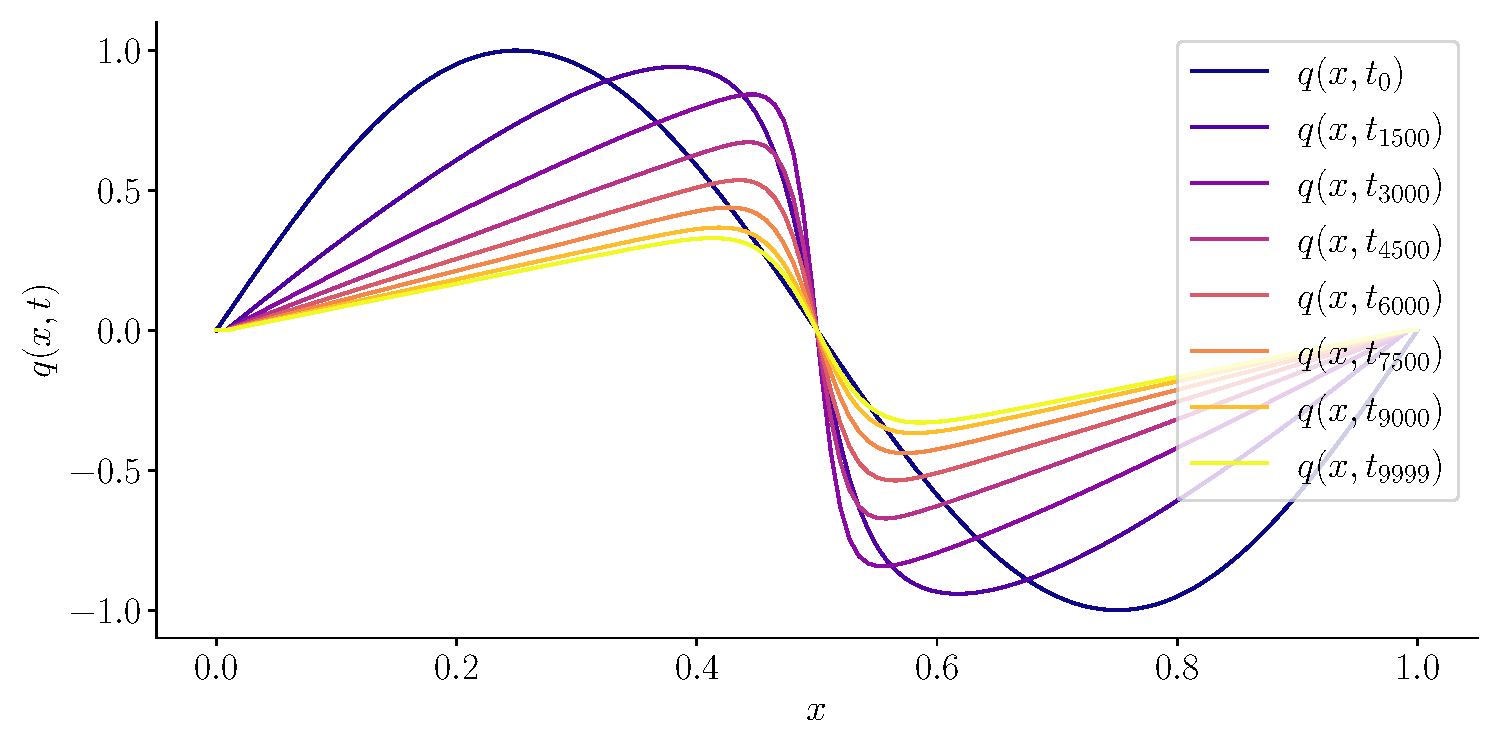
\includegraphics[width=0.8\textwidth]{figures/burgers_evol_001.pdf}
    \caption{Profiles \(q(x,t_k)\) at selected times \(t_k\).}
    \label{fig:burgers-surface}
  \end{subfigure}
  \\[1em]
  \begin{subfigure}[t]{0.56\textwidth}
    \centering
    \hspace{-1.5cm}
    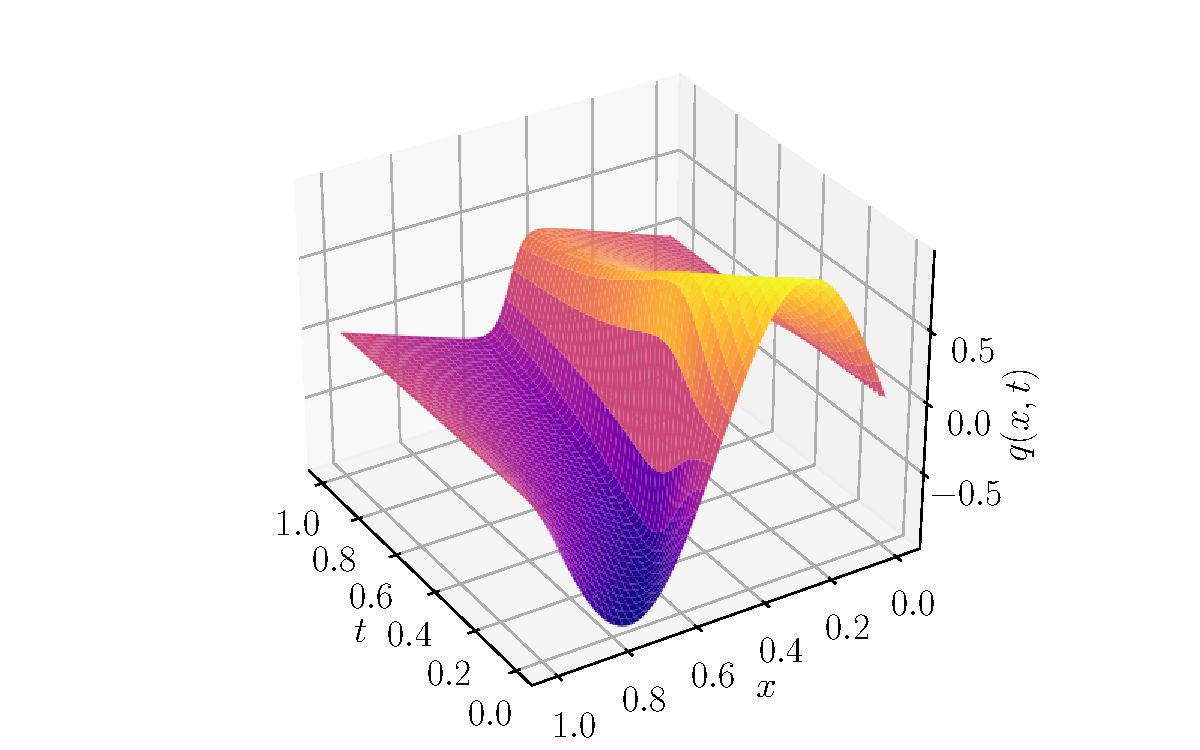
\includegraphics[width=\textwidth]{figures/burgers_sol_001.pdf}
    \caption{3D surface of \(q(x,t)\) for \(\nu=0.01\).}
    \label{fig:burgers-slices}
  \end{subfigure}
  \hspace{-1.5cm}
  \begin{subfigure}[t]{0.5\textwidth}
    \centering
    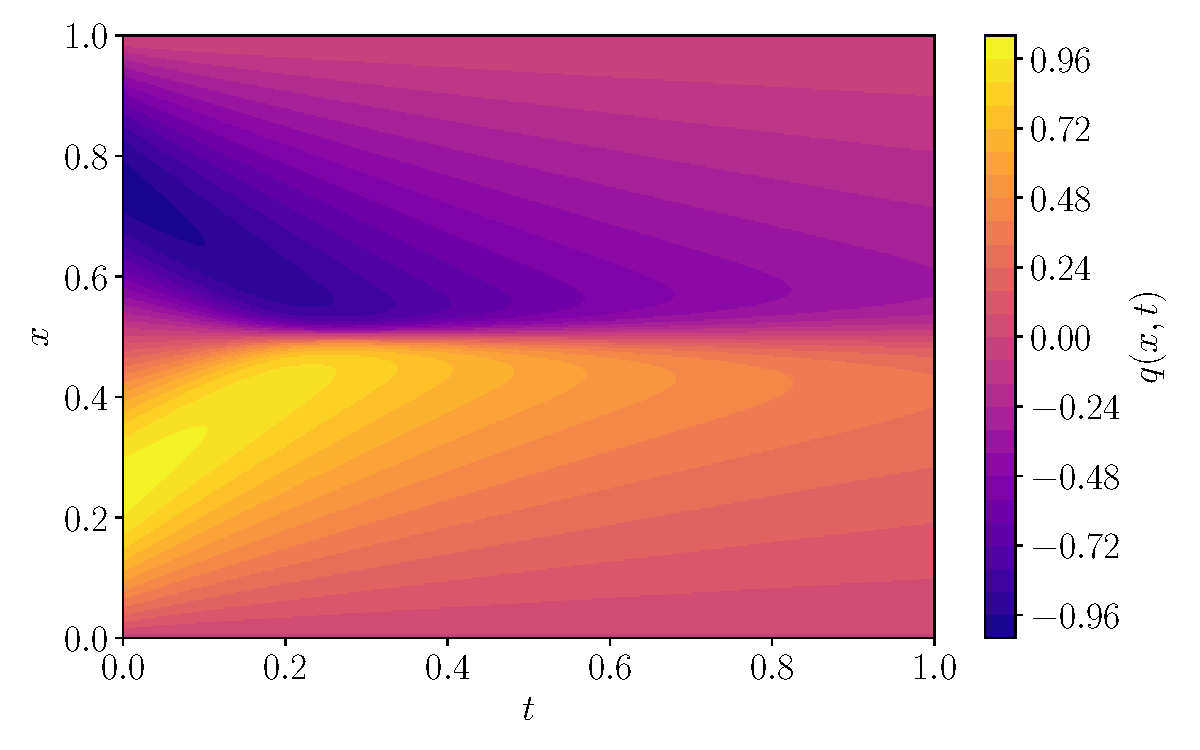
\includegraphics[width=\textwidth]{figures/heatmap_001.pdf}
    \caption{Space–time contour of \(q(x,t)\).}
    \label{fig:burgers-contour}
  \end{subfigure}
  \caption{Dynamics of the viscous Burgers’ equation used for data generation.}
  \label{fig:burgers-data}
\end{figure}

%%%%

For the Burgers’ dataset, Algorithm~\ref{algorithm_2} is trained on the time interval $t\in[0,0.5]$ and then used to predict over $t\in[0.5,1.0]$. We systematically reduce the number of snapshots to 100\% (10~000 points), 10\% (1~000 points), 1\% (100 points), and 0.2\% (20 points) of the original temporal grid. In each scenario, we estimate OpInf parameters with both second-order (\texttt{'ord2'}) and sixth-order (\texttt{'ord6'}) finite differences, applying an $L^2$-regularization weight $\xi=10^{-2}$.  

Figure~\ref{fig:five_by_two} displays, for each sampling level, the true reduced states $\hat{\mathbf{q}}_{\mathrm{true}}$ (solid) versus the predicted trajectories $\hat{\mathbf{q}}_{\mathrm{pred}}$ (dashed) for both the OpInf and adjoint-trained models. Even at extreme sampling sparsity, the adjoint method produces predictions that are visually indistinguishable from those of OpInf, demonstrating its resilience in the absence of noise.

\newpage

%%%%%%%%%%%%%%%%%%%%%%%%%%%%%%%%% DATA DENSITY REDUCTION  - BURGERS %%%%%%%%%%%%%%%%%%%%%%%%%%%%%%%%%

\subsection*{Data Density Reduction}

\vspace{1.0cm}

\begin{figure}[h!]
  \centering
  \begin{subfigure}[c]{0.49\textwidth}
      \centering
      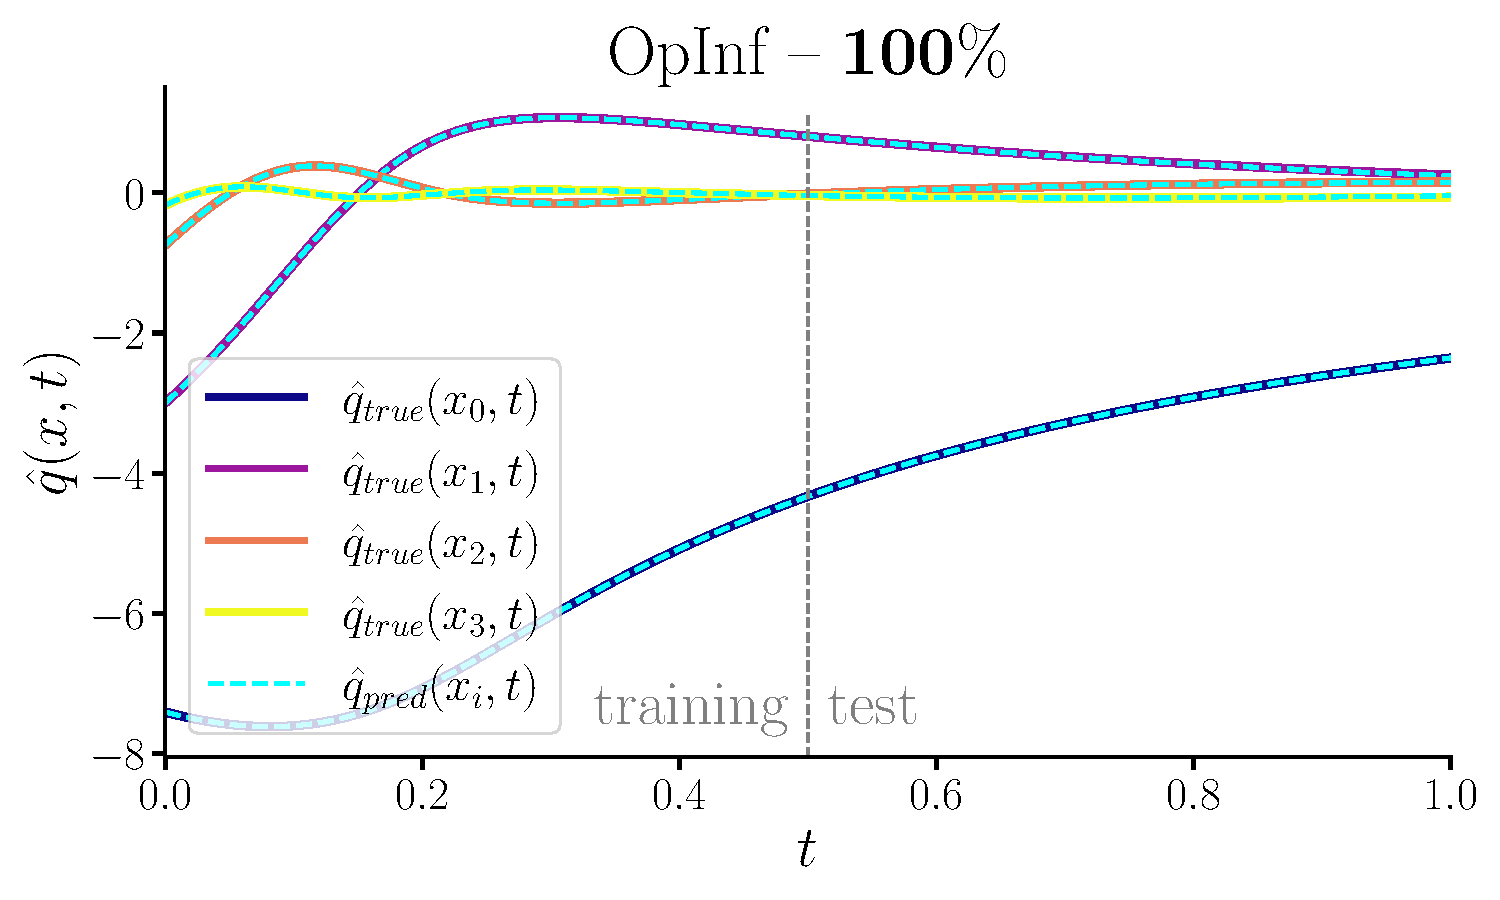
\includegraphics[width=\linewidth]{rom_data_density_100_OpInf.pdf}
  \end{subfigure}
  \begin{subfigure}[c]{0.49\textwidth}
      \centering
      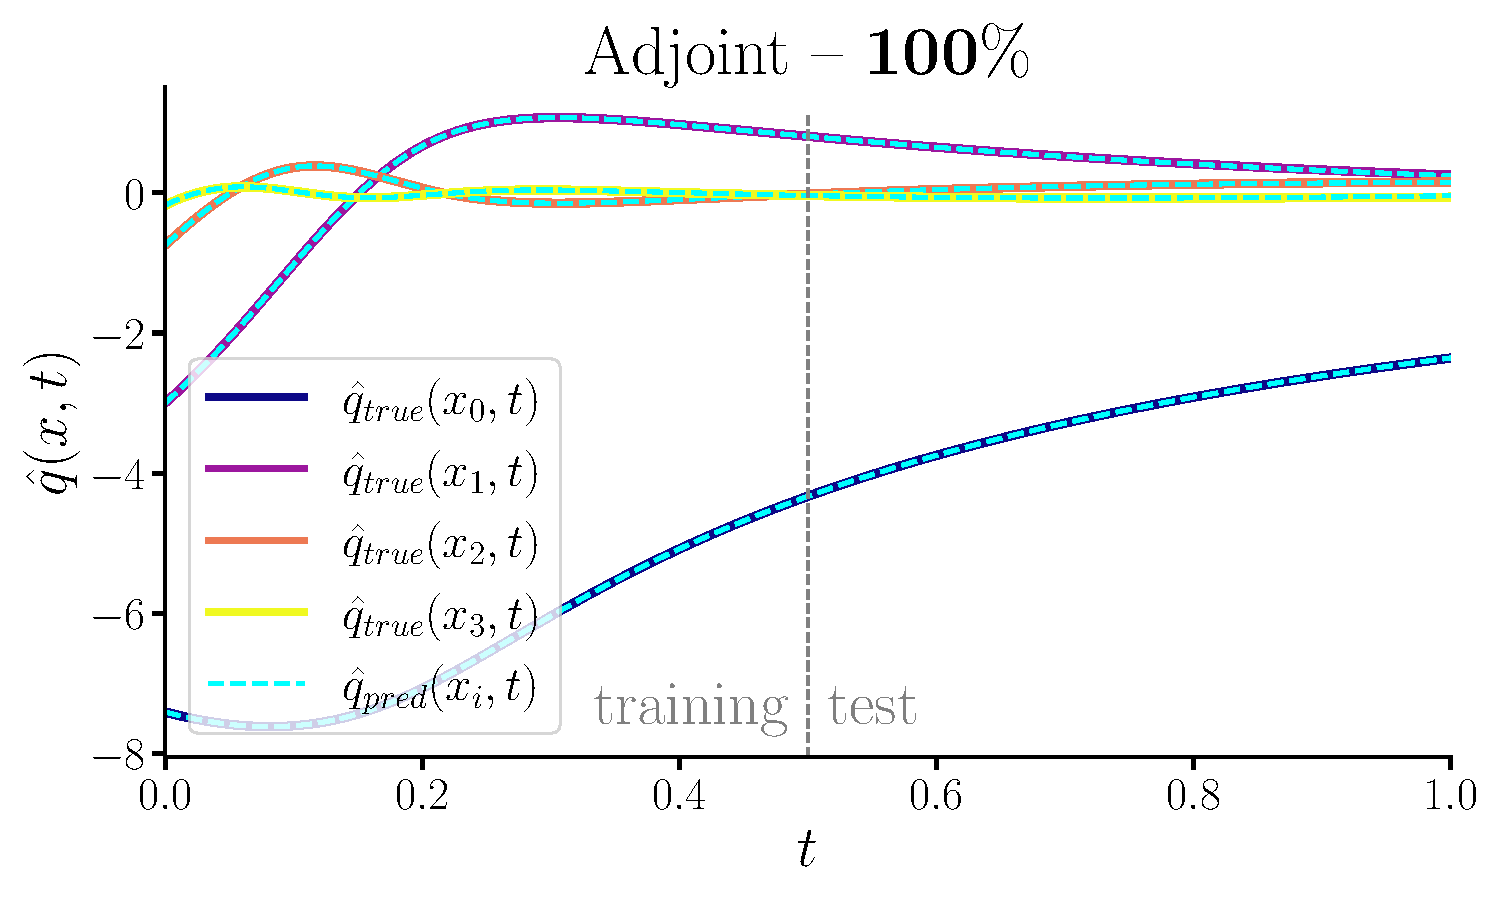
\includegraphics[width=\linewidth]{rom_data_density_100_Adj.pdf}
  \end{subfigure} \\[1ex]
    
  \begin{subfigure}[c]{0.49\textwidth}
      \centering
      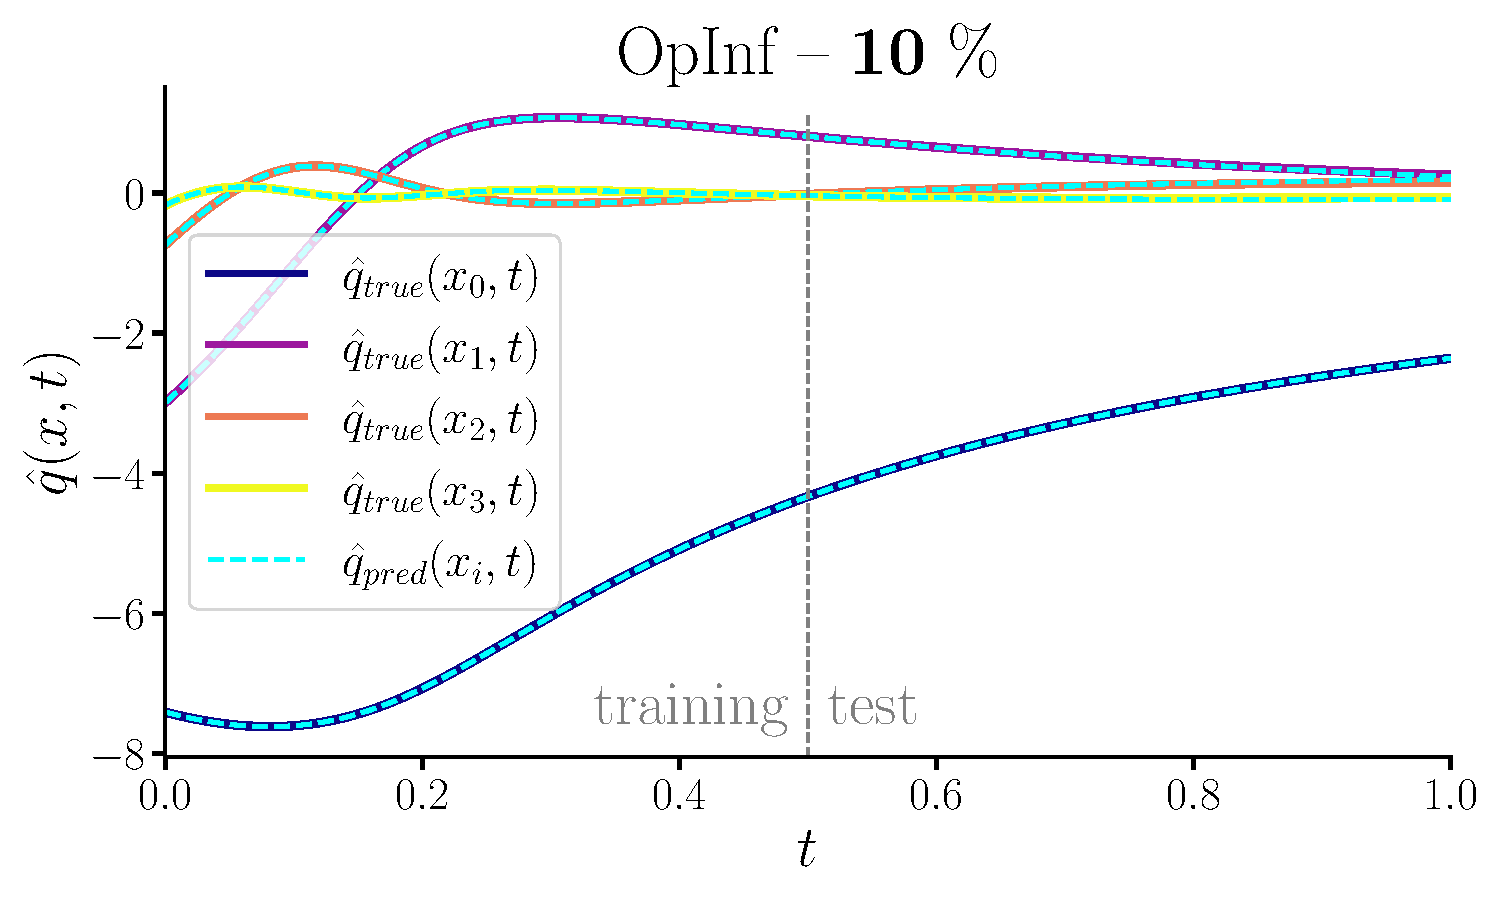
\includegraphics[width=\linewidth]{rom_data_density_10_OpInf.pdf}
  \end{subfigure} 
  \begin{subfigure}[c]{0.49\textwidth}
      \centering
      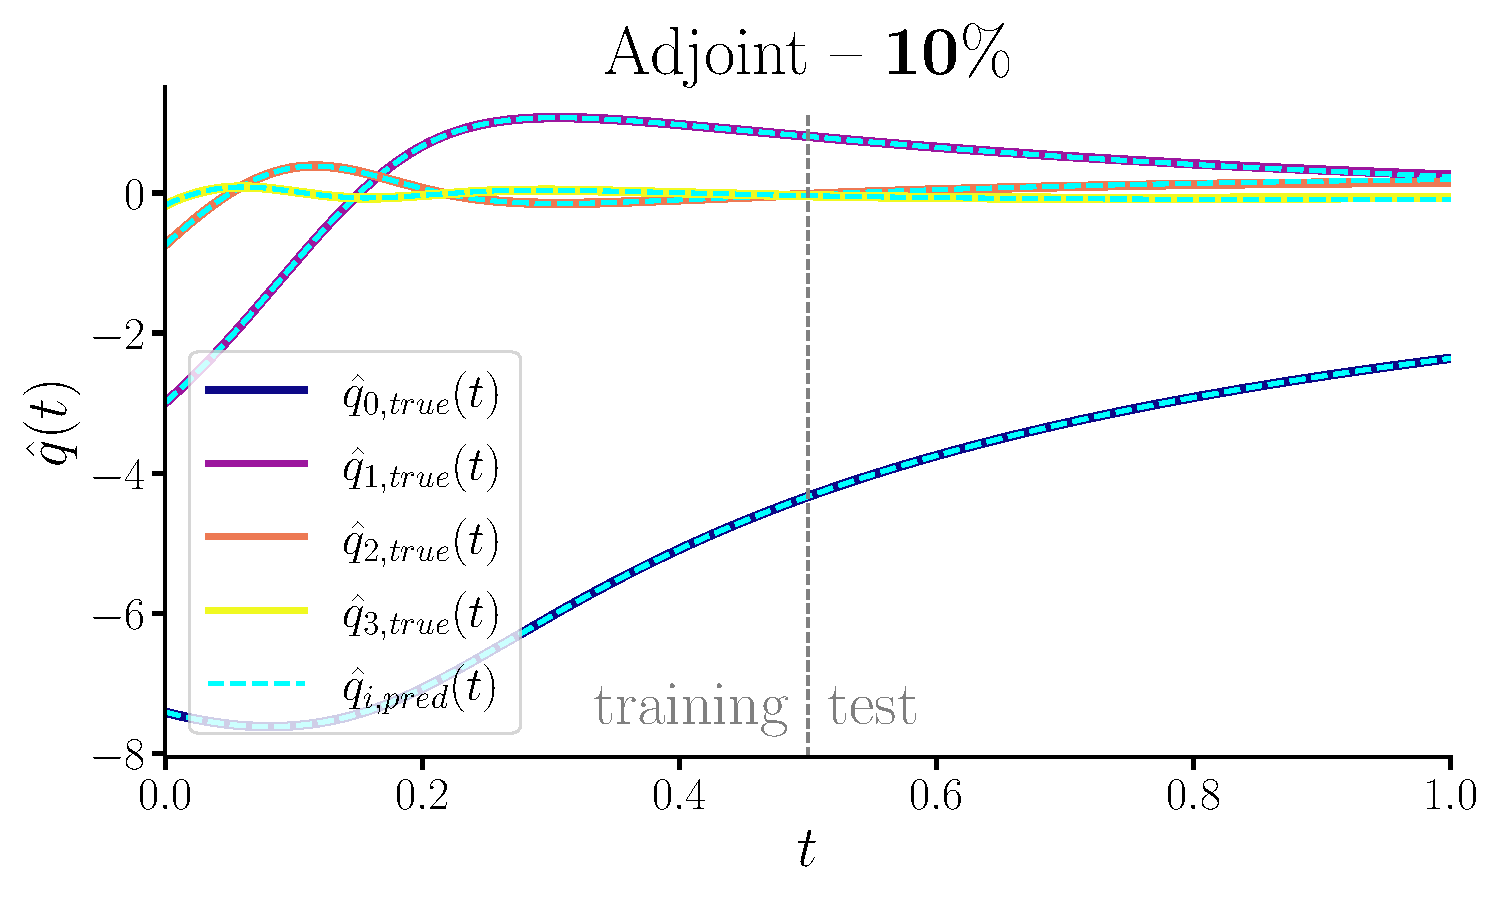
\includegraphics[width=\linewidth]{figures/rom_data_density_10_Adj.pdf}
  \end{subfigure} \\[1ex]
    
  \begin{subfigure}[c]{0.49\textwidth}
      \centering
      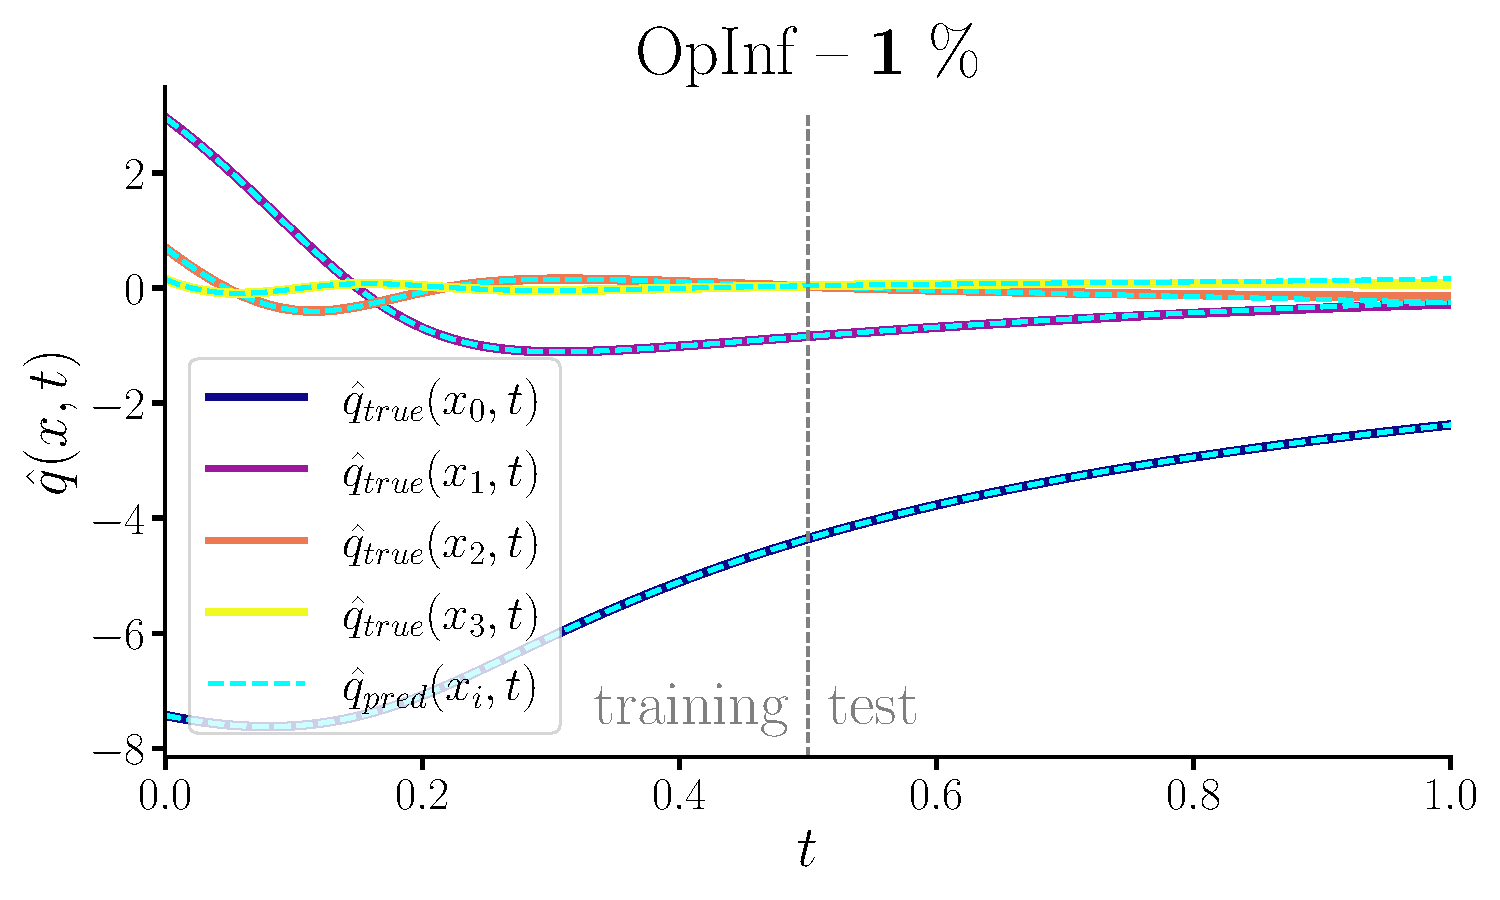
\includegraphics[width=\linewidth]{rom_data_density_1_OpInf.pdf}
  \end{subfigure} 
  \begin{subfigure}[c]{0.49\textwidth}
      \centering
      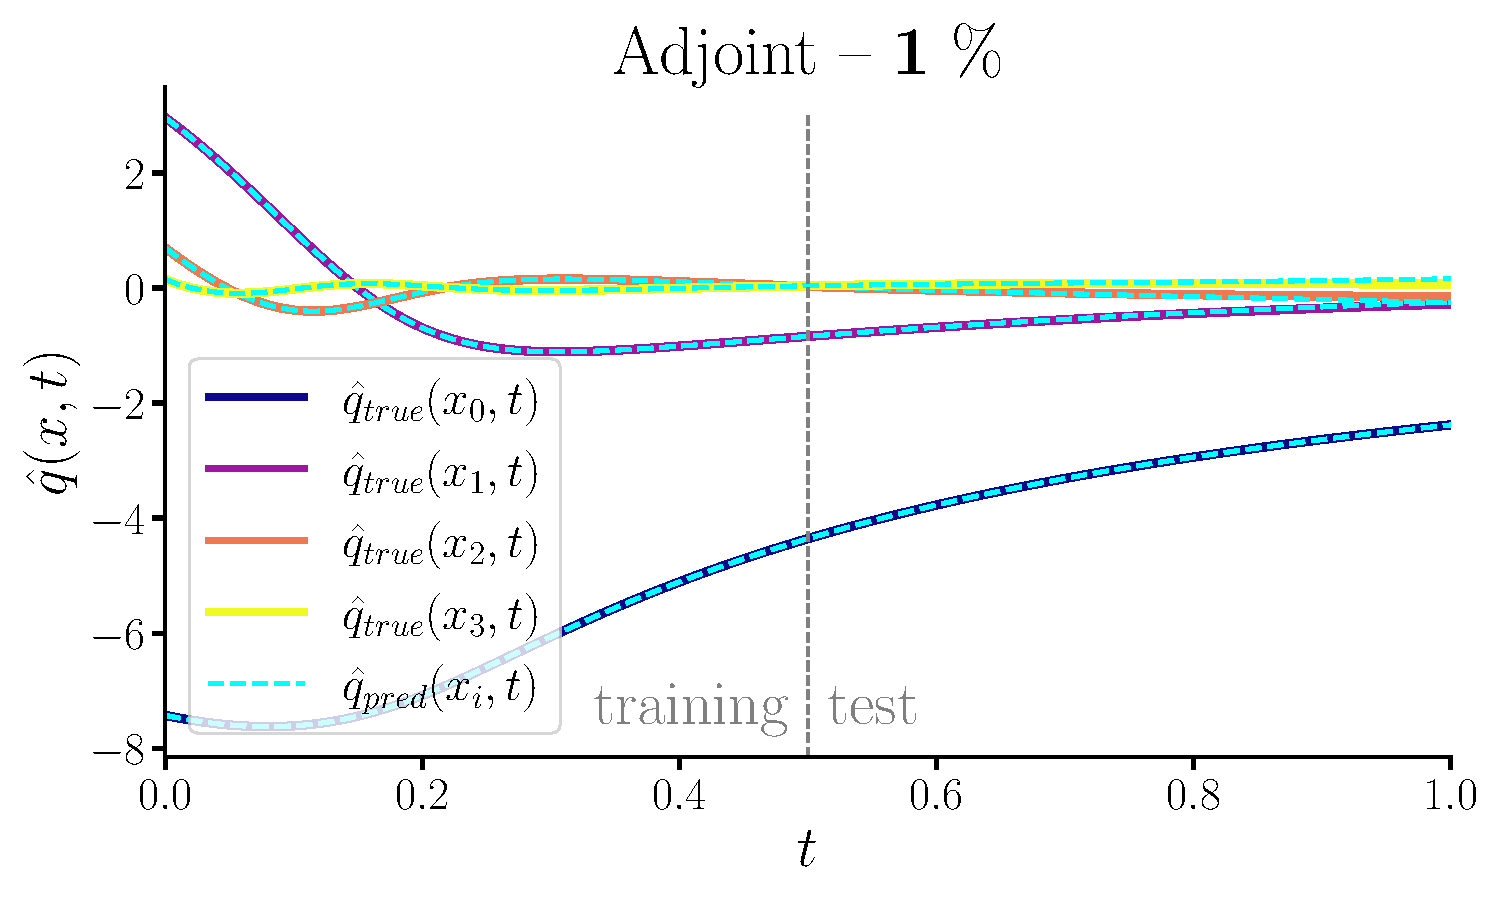
\includegraphics[width=\linewidth]{rom_data_density_1_Adj.pdf}
  \end{subfigure} \\[1ex]
    
  \begin{subfigure}[c]{0.49\textwidth}
      \centering
      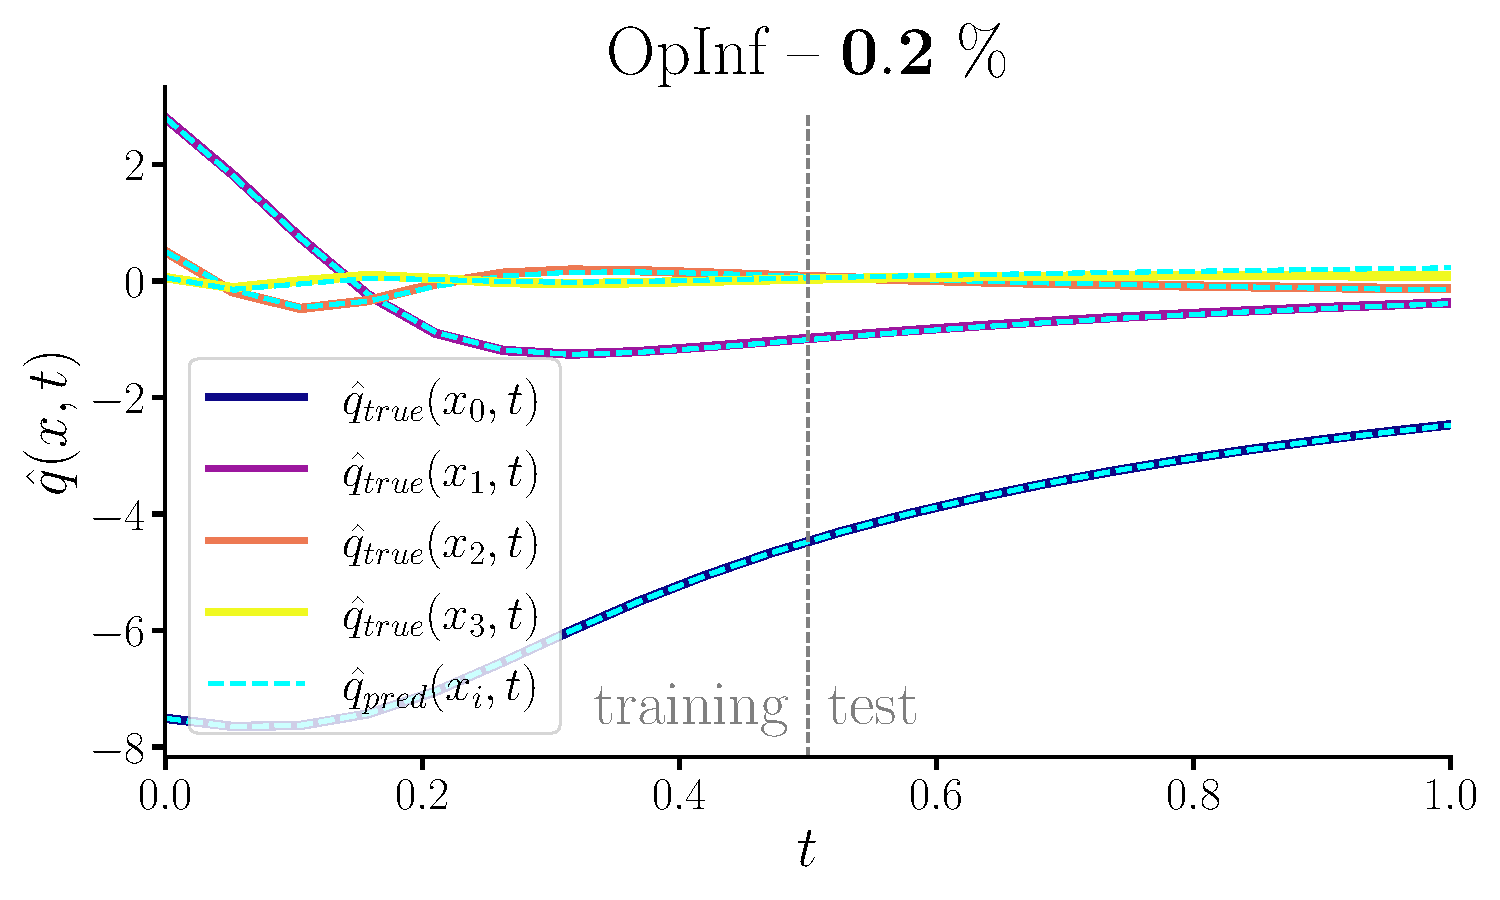
\includegraphics[width=\linewidth]{rom_data_density_02_OpInf.pdf}
  \end{subfigure} 
  \begin{subfigure}[c]{0.49\textwidth}
      \centering
      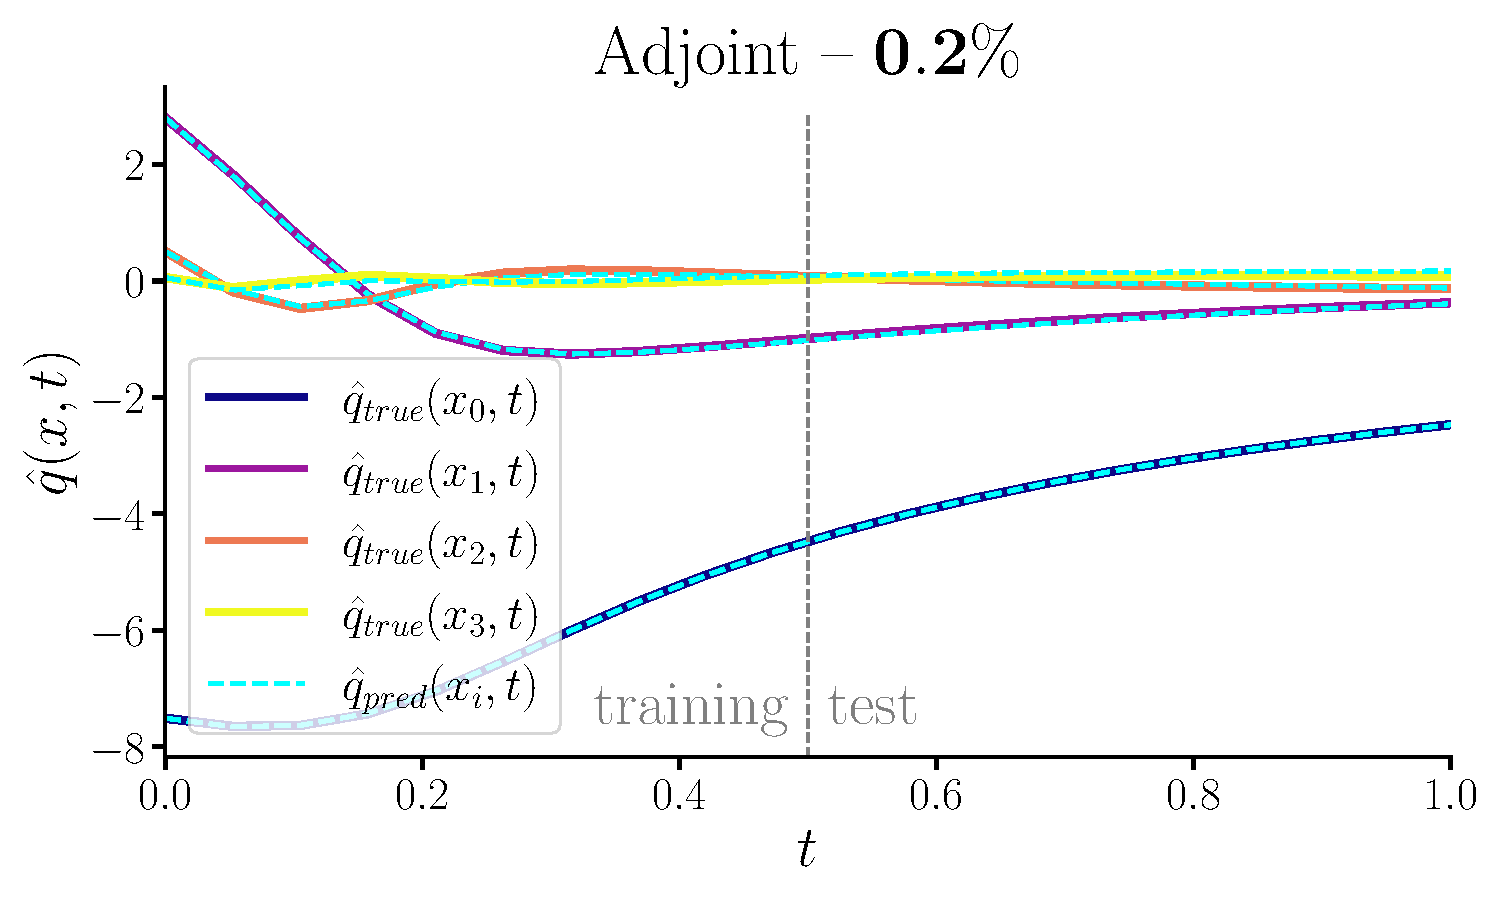
\includegraphics[width=\linewidth]{rom_data_density_02_Adj.pdf}
  \end{subfigure} \\[1ex]
  \caption{Data density reduction results for the Burgers' Equation synthetic experiment.}
  \label{fig:five_by_two}
\end{figure}

\newpage

%%%%%% Prediction Error vs. Time (data density - Burgers) %%%%%%

To quantify the impact of training data sparsity, we compute the prediction error in the test region $t\in[0.5,1]$ for each sampling density. Specifically, we solve the ROM-OpInf initial value problem with the learned operators and compare the trajectories against the true reduced states for each sampling level (100\%, 10\%, 1\%, 0.2\% respectively):\\
  $$\|\hat{\mathbf{q}}_{\mathrm{true}}(t) - \hat{\mathbf{q}}_{\mathrm{pred}}(t)\|_2,
  \quad t\in[0.5,1].$$
Figure~\ref{fig:twobytwo} compares the OpInf and adjoint error curves across all sampling levels. The adjoint method produces errors similar to or even lower than when the sixth-order stencil is used, confirming its accuracy capturing time-derivative information under limited data.

\vspace{0.7cm}

\begin{figure}[h!]
  \centering
  
  % First row of subfigures
  \begin{subfigure}[b]{0.48\textwidth}
    \centering
    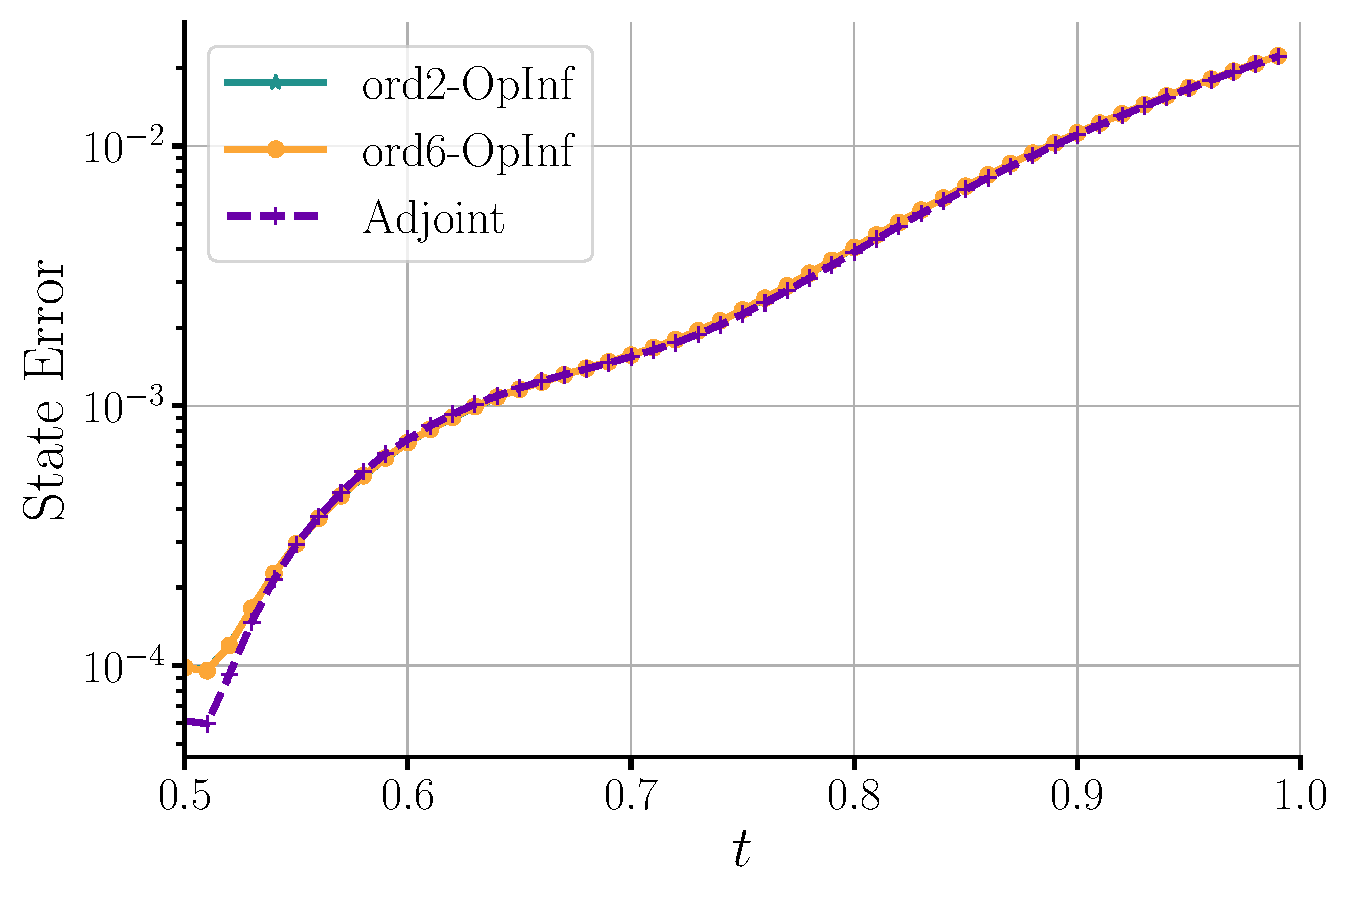
\includegraphics[width=\linewidth]{pred_error_vs_time_data_density_100.pdf}
    \caption{100\% of the data.}
    \label{fig:image1}
  \end{subfigure}
  \quad
  \begin{subfigure}[b]{0.48\textwidth}
    \centering
    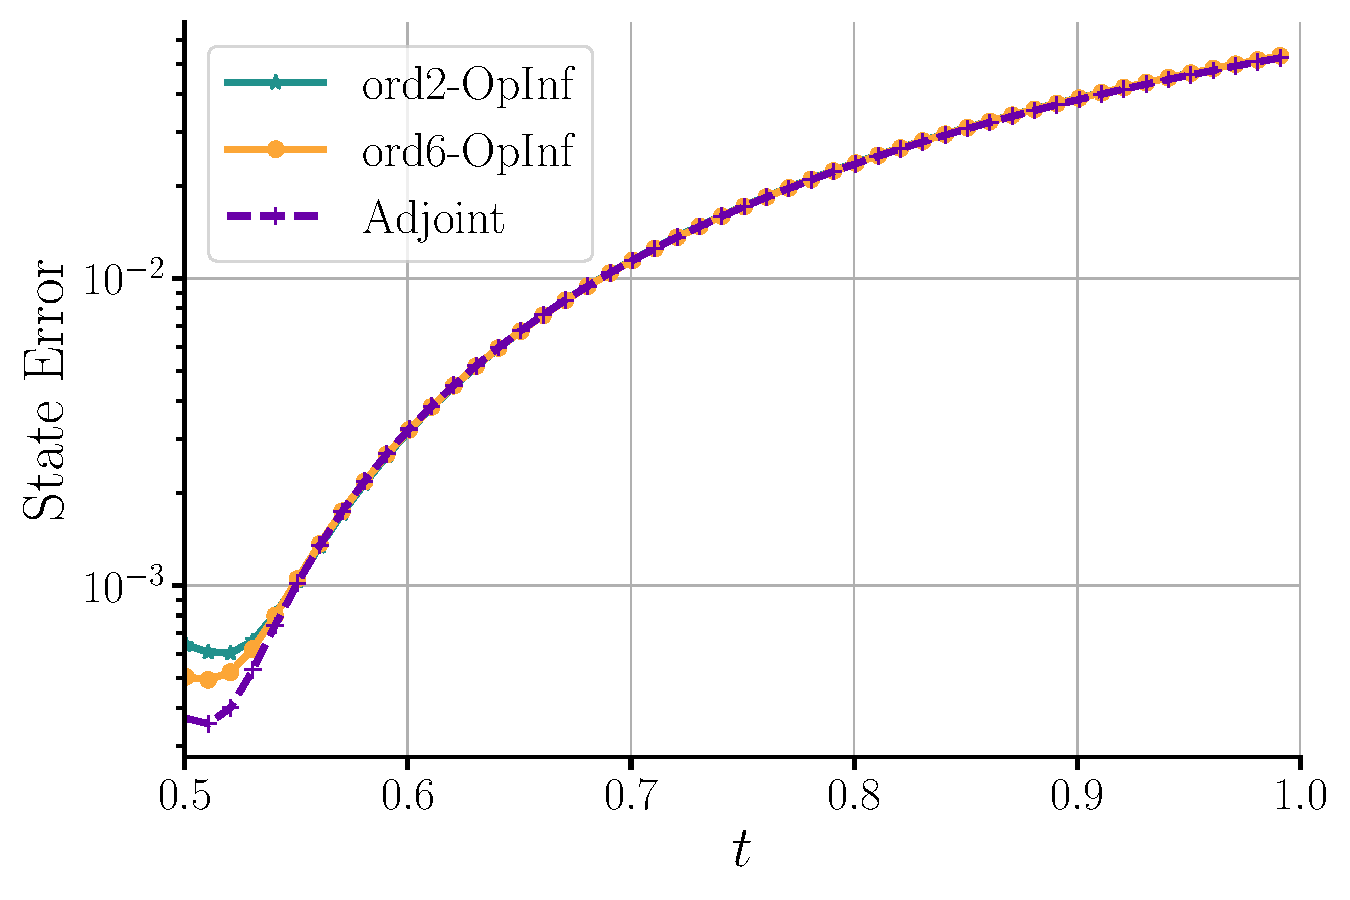
\includegraphics[width=\linewidth]{pred_error_vs_time_data_density_10.pdf}
    \caption{10\% of the data.}
    \label{fig:image2}
  \end{subfigure}
  
  \vskip\baselineskip
  
  % Second row of subfigures
  \begin{subfigure}[b]{0.48\textwidth}
    \centering
    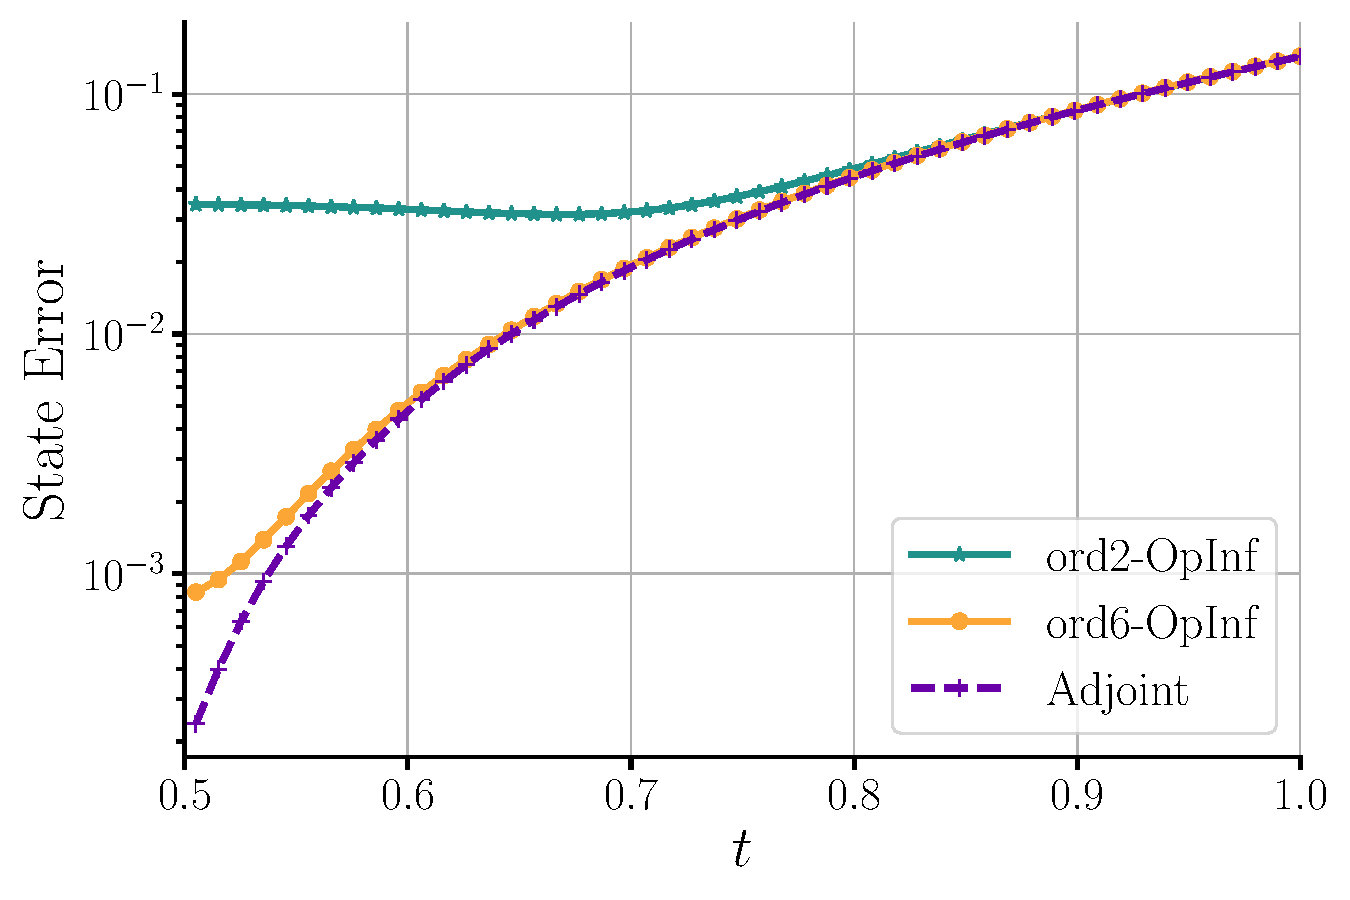
\includegraphics[width=\linewidth]{pred_error_vs_time_data_density_1.pdf}
    \caption{1\% of the data.}
    \label{fig:image3}
  \end{subfigure}
  \quad
  \begin{subfigure}[b]{0.48\textwidth}
    \centering
    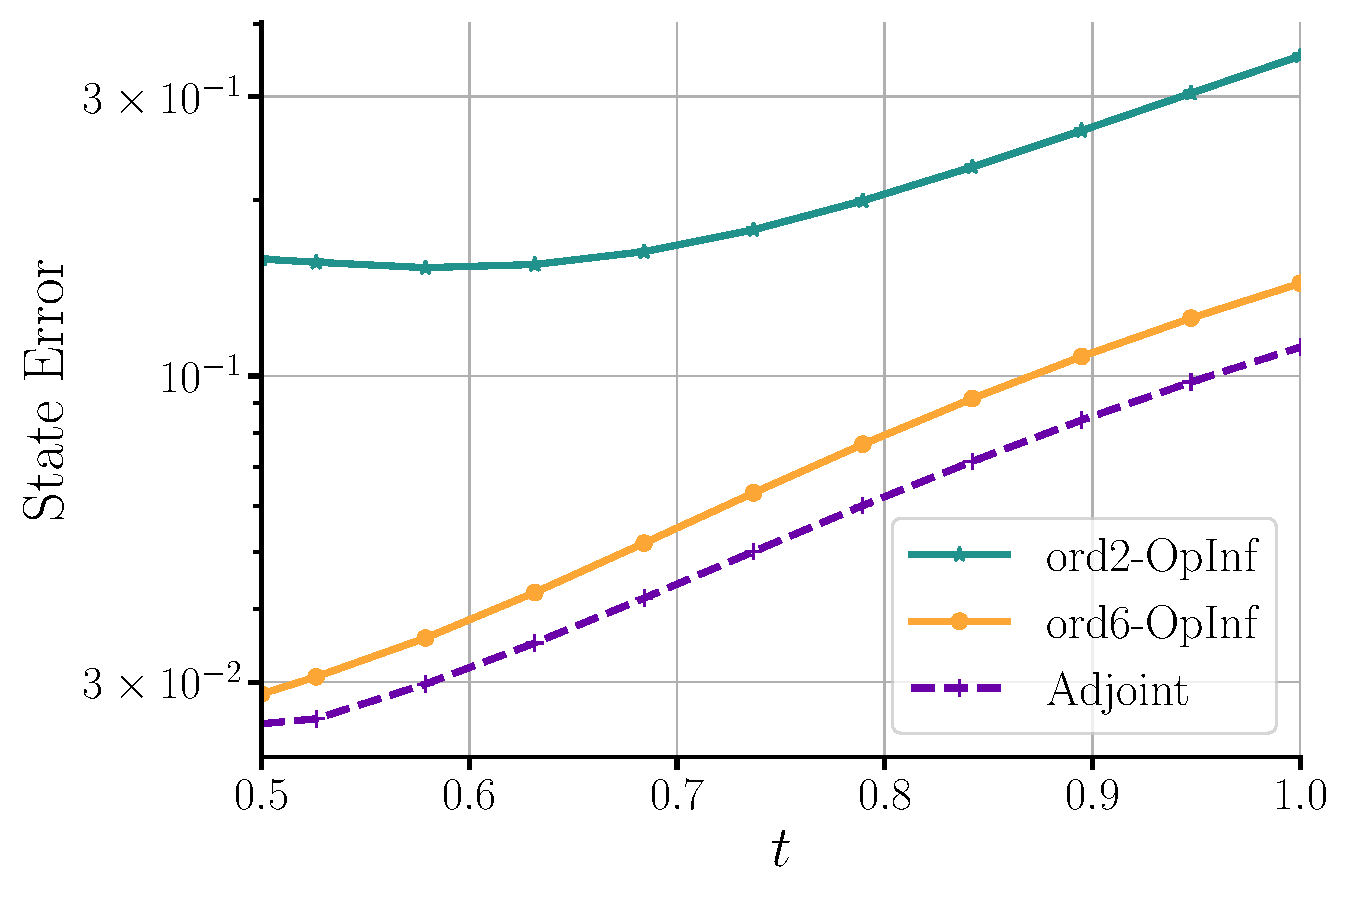
\includegraphics[width=\linewidth]{pred_error_vs_time_data_density_02.pdf}
    \caption{0.2\% of the data.}
    \label{fig:image4}
  \end{subfigure}
  
  \caption{Prediction error vs. time for each data density reduction run in the Burgers' Equation experiment.}
  \label{fig:twobytwo}
\end{figure}

\newpage

%%%%%% Relative Error vs. Time (data density - Burgers) %%%%%%

Figure~\ref{fig:twobytwo2} shows the relative error\\
$$\frac{\|\hat{\mathbf{q}}_{\mathrm{true}}(t) - \hat{\mathbf{q}}_{\mathrm{pred}}(t)\|_2}
       {\|\hat{\mathbf{q}}_{\mathrm{true}}(t)\|_2},
  \quad t\in[0,1],$$
as a function of the ROM dimension $r$. Again, each subplot corresponds to one of the four sampling densities. Both methods exhibit the expected decay in relative error with increasing $r$. However, in the most extreme sparsity case (0.2\%), the adjoint-trained model achieves marginally lower errors, suggesting it can construct more efficient reduced bases when snapshot information is scarce.

\vspace{0.7cm}

\begin{figure}[h!]
  \centering
  
  % First row of subfigures
  \begin{subfigure}[b]{0.48\textwidth}
    \centering
    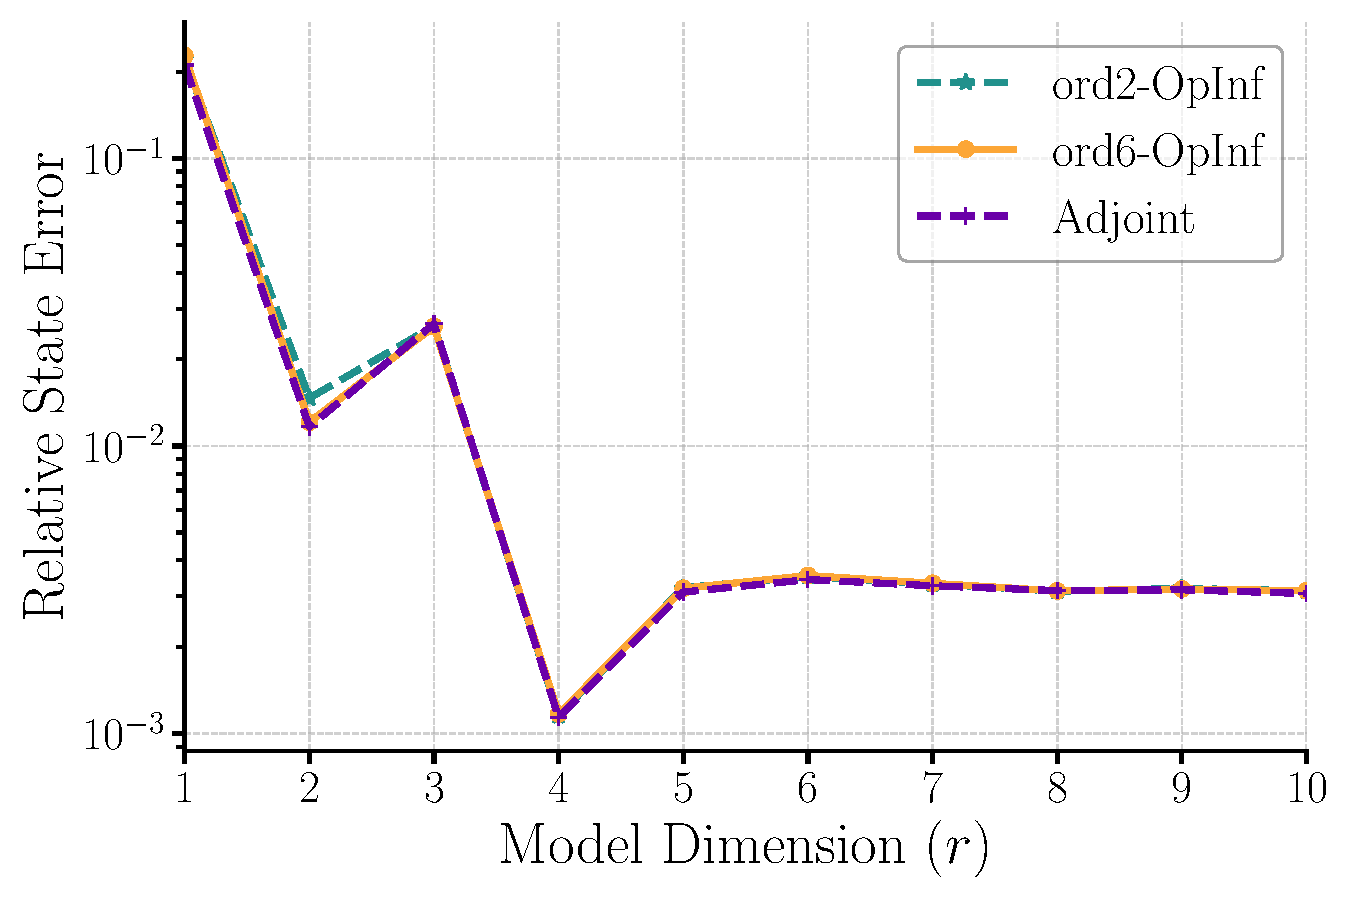
\includegraphics[width=\linewidth]{rel_error_vs_r_data_density_100.pdf}
    \caption{100\% of the data.}
    \label{fig:image1}
  \end{subfigure}
  \quad
  \begin{subfigure}[b]{0.48\textwidth}
    \centering
    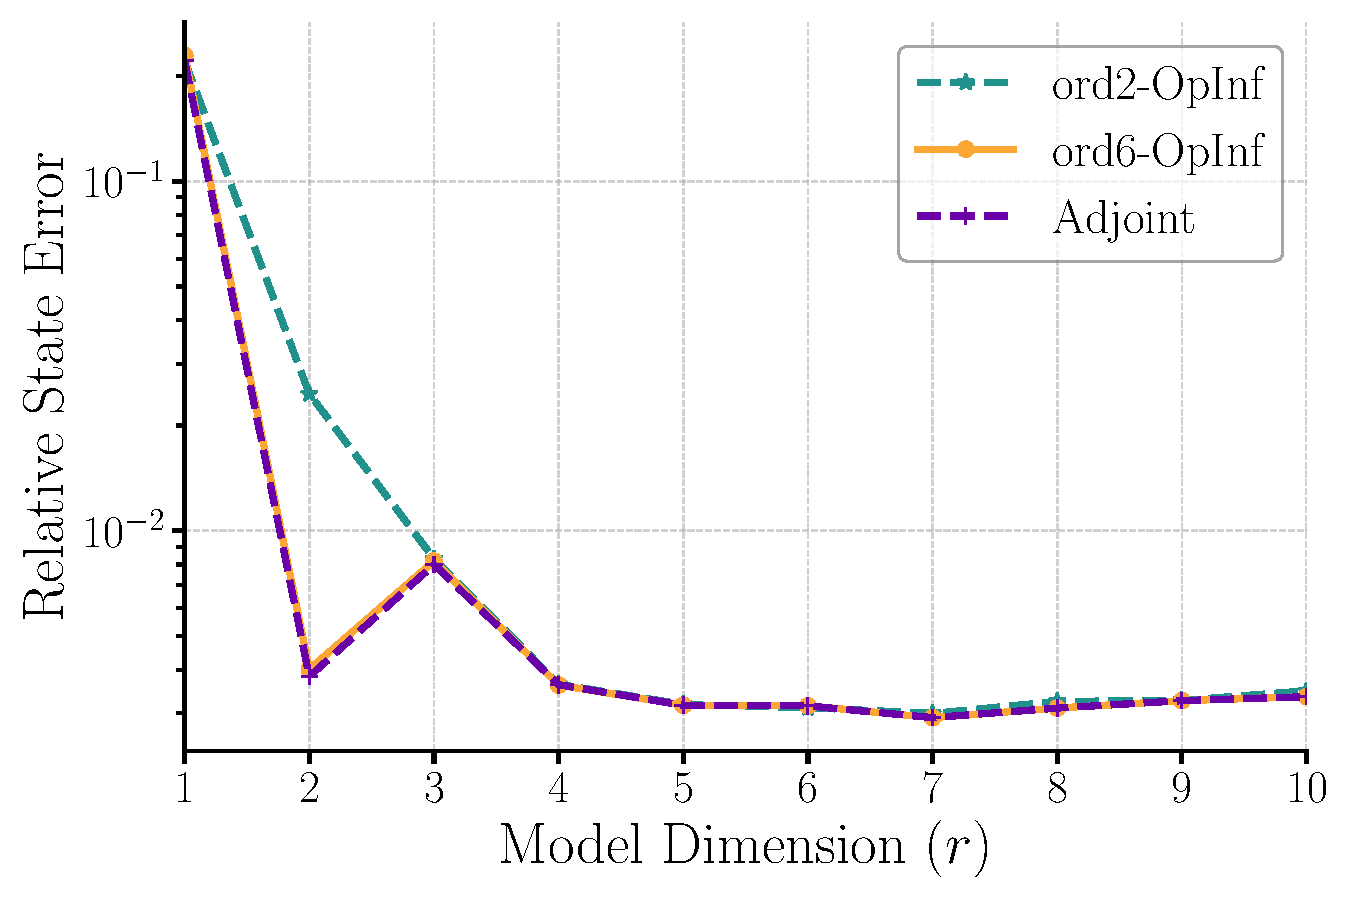
\includegraphics[width=\linewidth]{rel_error_vs_r_data_density_10.pdf}
    \caption{10\% of the data.}
    \label{fig:image2}
  \end{subfigure}
  
  \vskip\baselineskip
  
  % Second row of subfigures
  \begin{subfigure}[b]{0.48\textwidth}
    \centering
    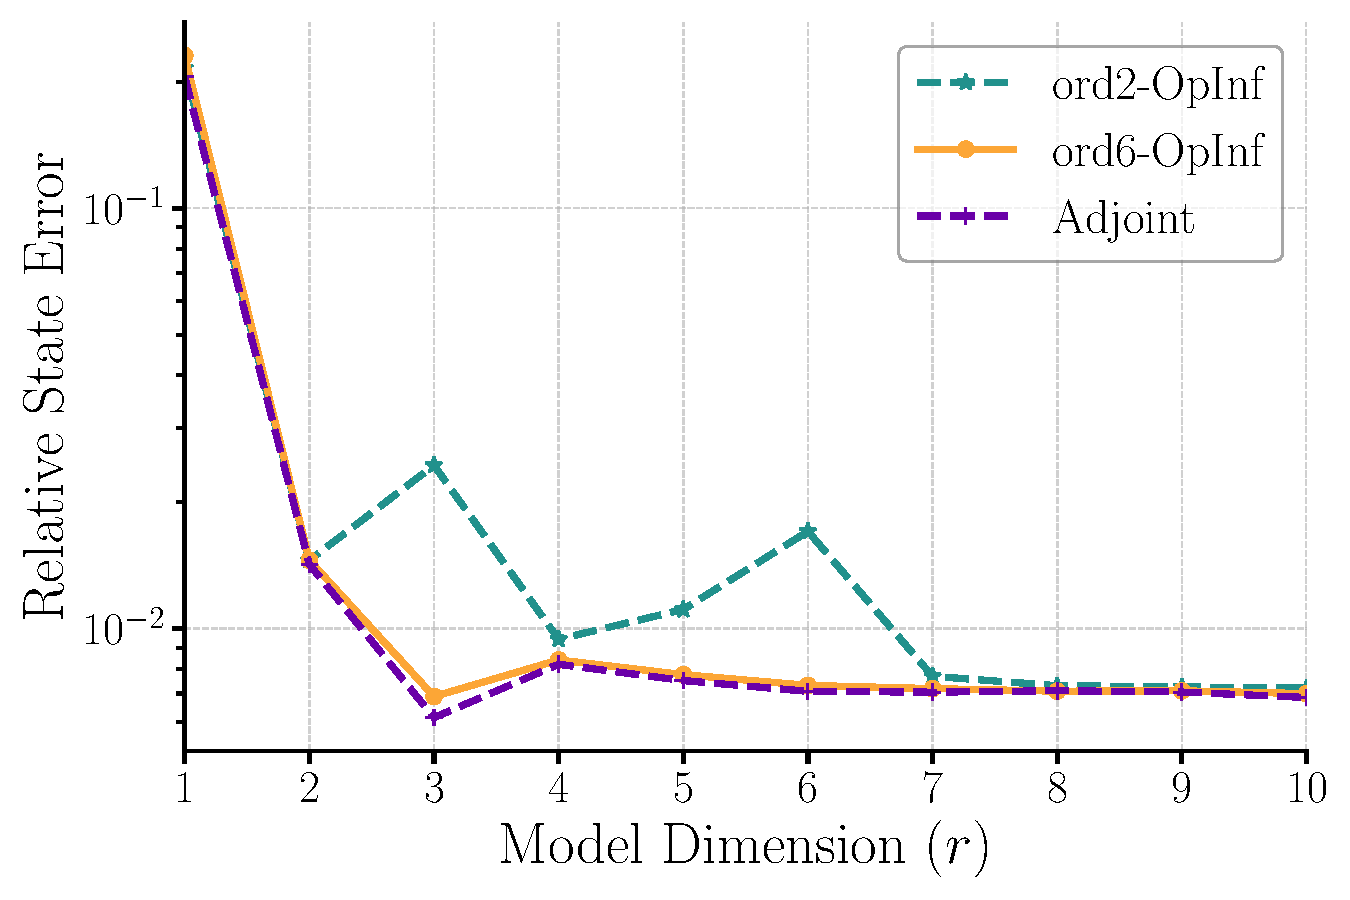
\includegraphics[width=\linewidth]{rel_error_vs_r_data_density_1.pdf}
    \caption{1\% of the data.}
    \label{fig:image3}
  \end{subfigure}
  \quad
  \begin{subfigure}[b]{0.48\textwidth}
    \centering
    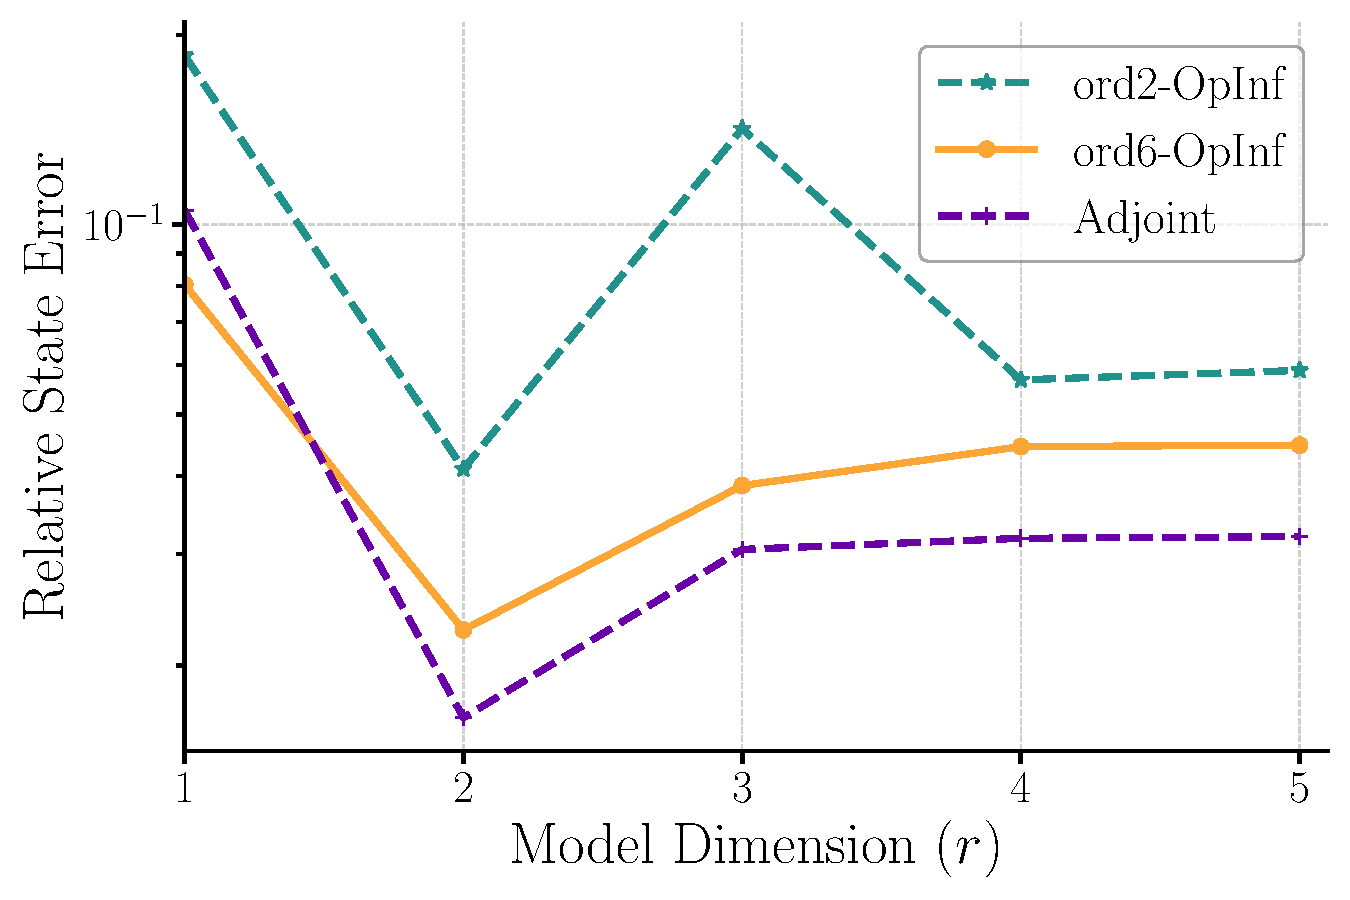
\includegraphics[width=\linewidth]{rel_error_vs_r_data_density_02.pdf}
    \caption{0.2\% of the data.}
    \label{fig:image4}
  \end{subfigure}
  
  \caption{Relative error vs. $r$ for each data density reduction run in the Burgers' Equation experiment.}
  \label{fig:twobytwo2}
\end{figure}

\newpage

%%%%%%%%%%%%%%%%%%%%%%%%%%%%%%%%% NOISE PERTURBATION %%%%%%%%%%%%%%%%%%%%%%%%%%%%%%%%%%

\subsection*{Noise Perturbation}

\vspace{1.0cm}

\begin{figure}[h!]
  \centering
  \begin{subfigure}[c]{0.49\textwidth}
      \centering
      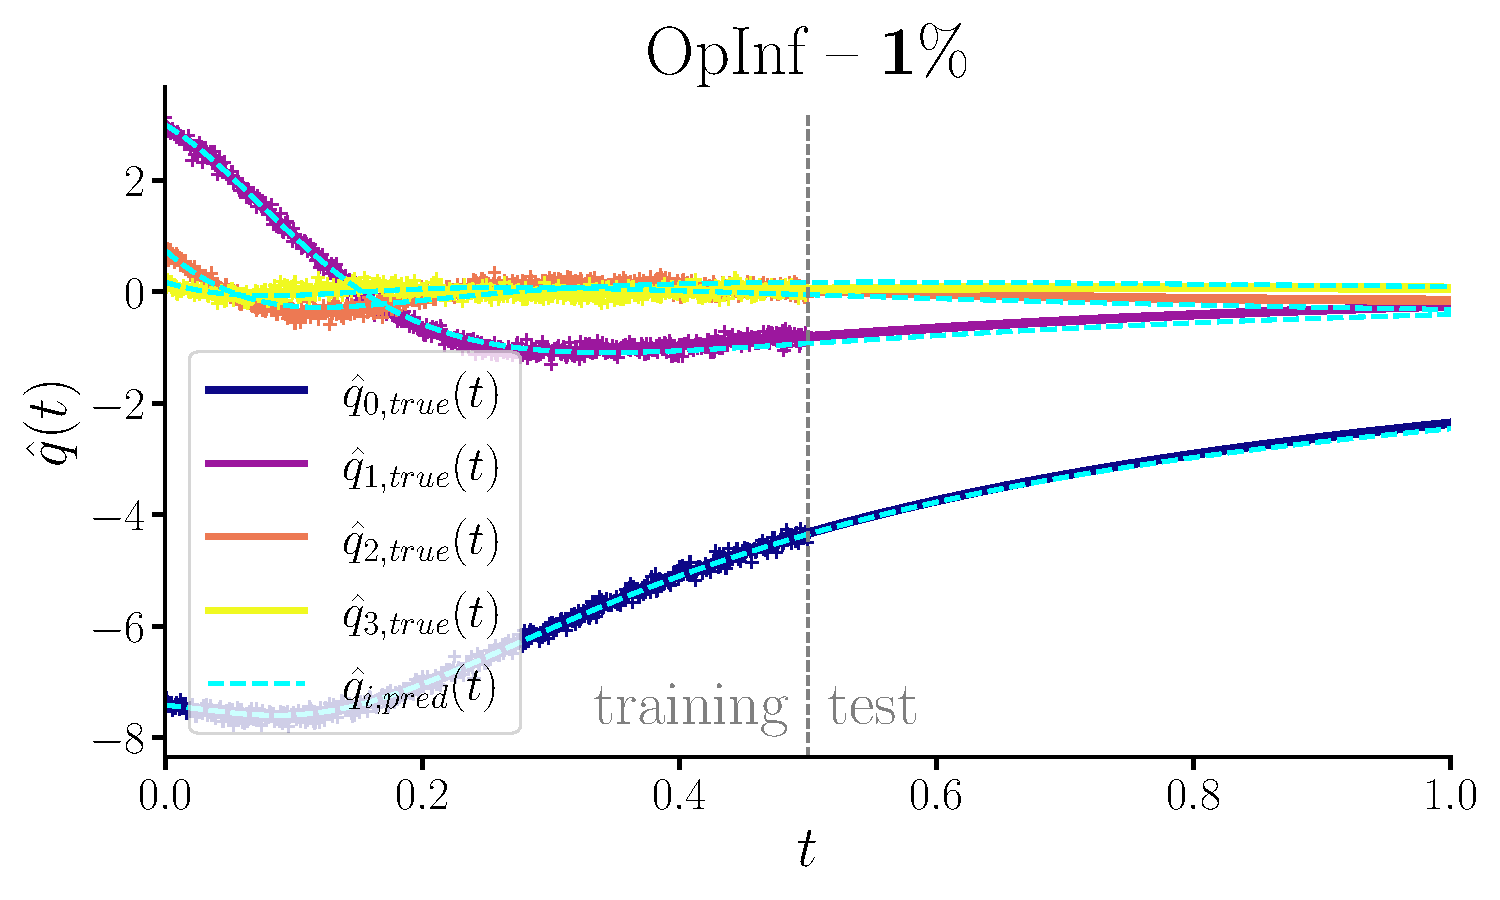
\includegraphics[width=\linewidth]{rom_noise_1_OpInf.pdf}
  \end{subfigure}
  \begin{subfigure}[c]{0.49\textwidth}
      \centering
      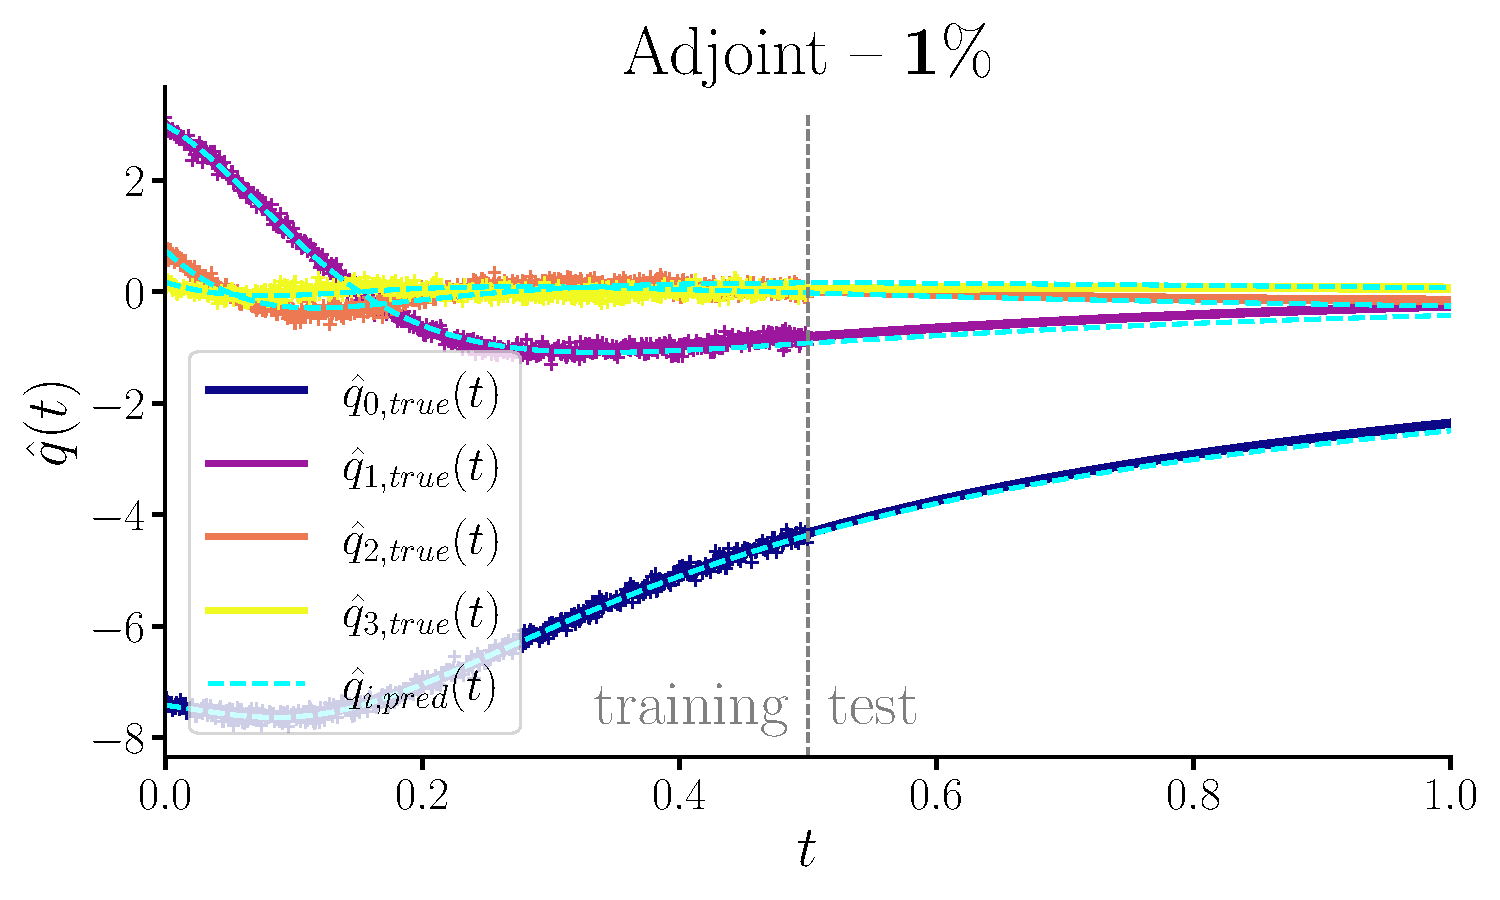
\includegraphics[width=\linewidth]{rom_noise_1_Adj.pdf}
  \end{subfigure} \\[1ex]
    
  \begin{subfigure}[c]{0.49\textwidth}
      \centering
      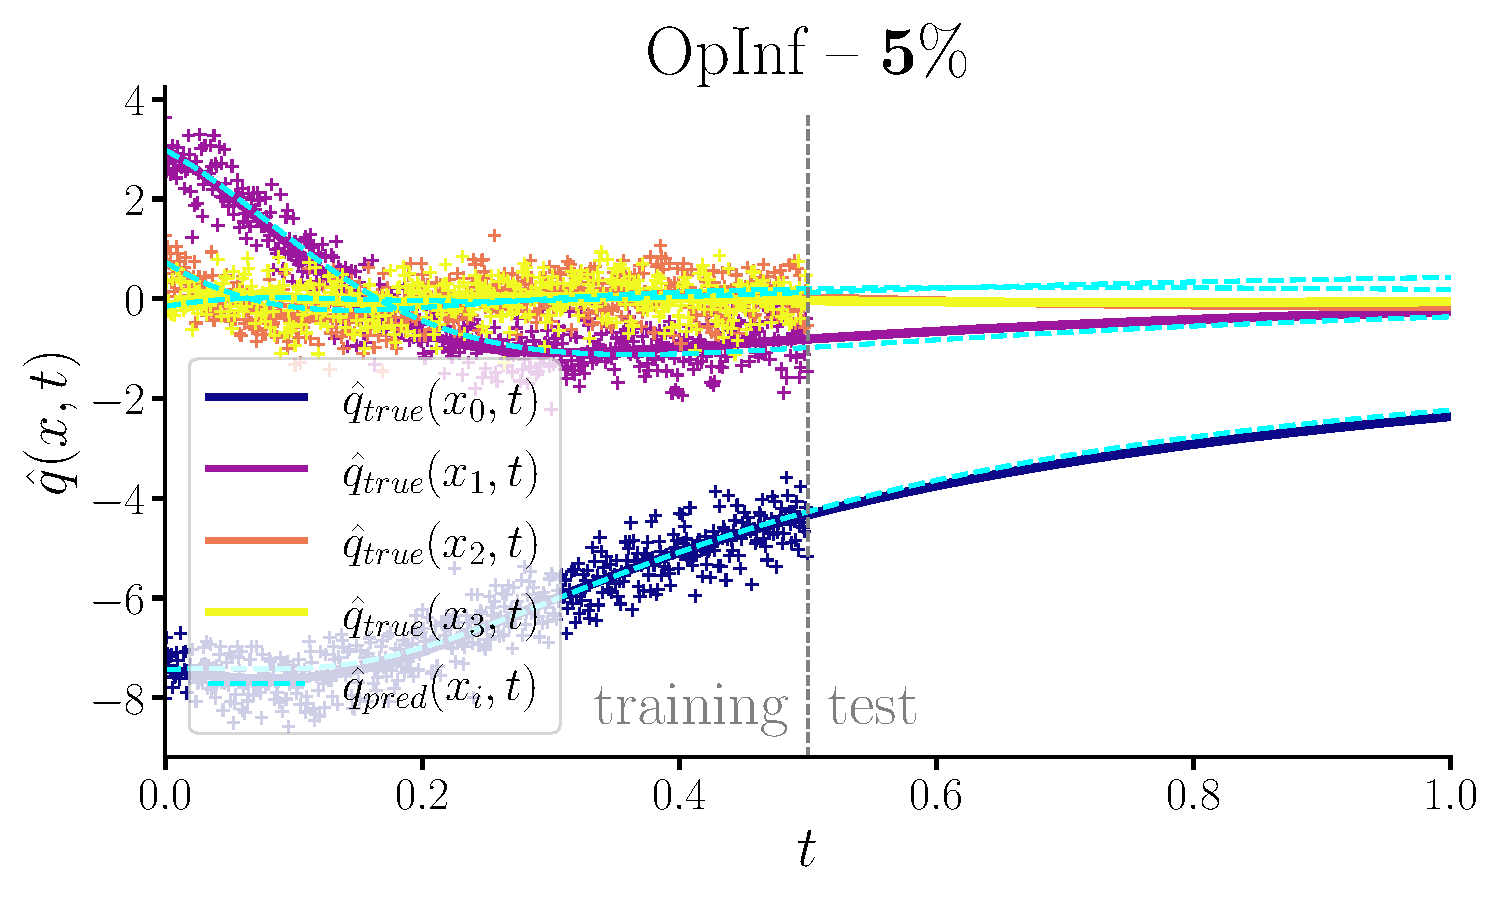
\includegraphics[width=\linewidth]{rom_noise_5_OpInf.pdf}
  \end{subfigure} 
  \begin{subfigure}[c]{0.49\textwidth}
      \centering
      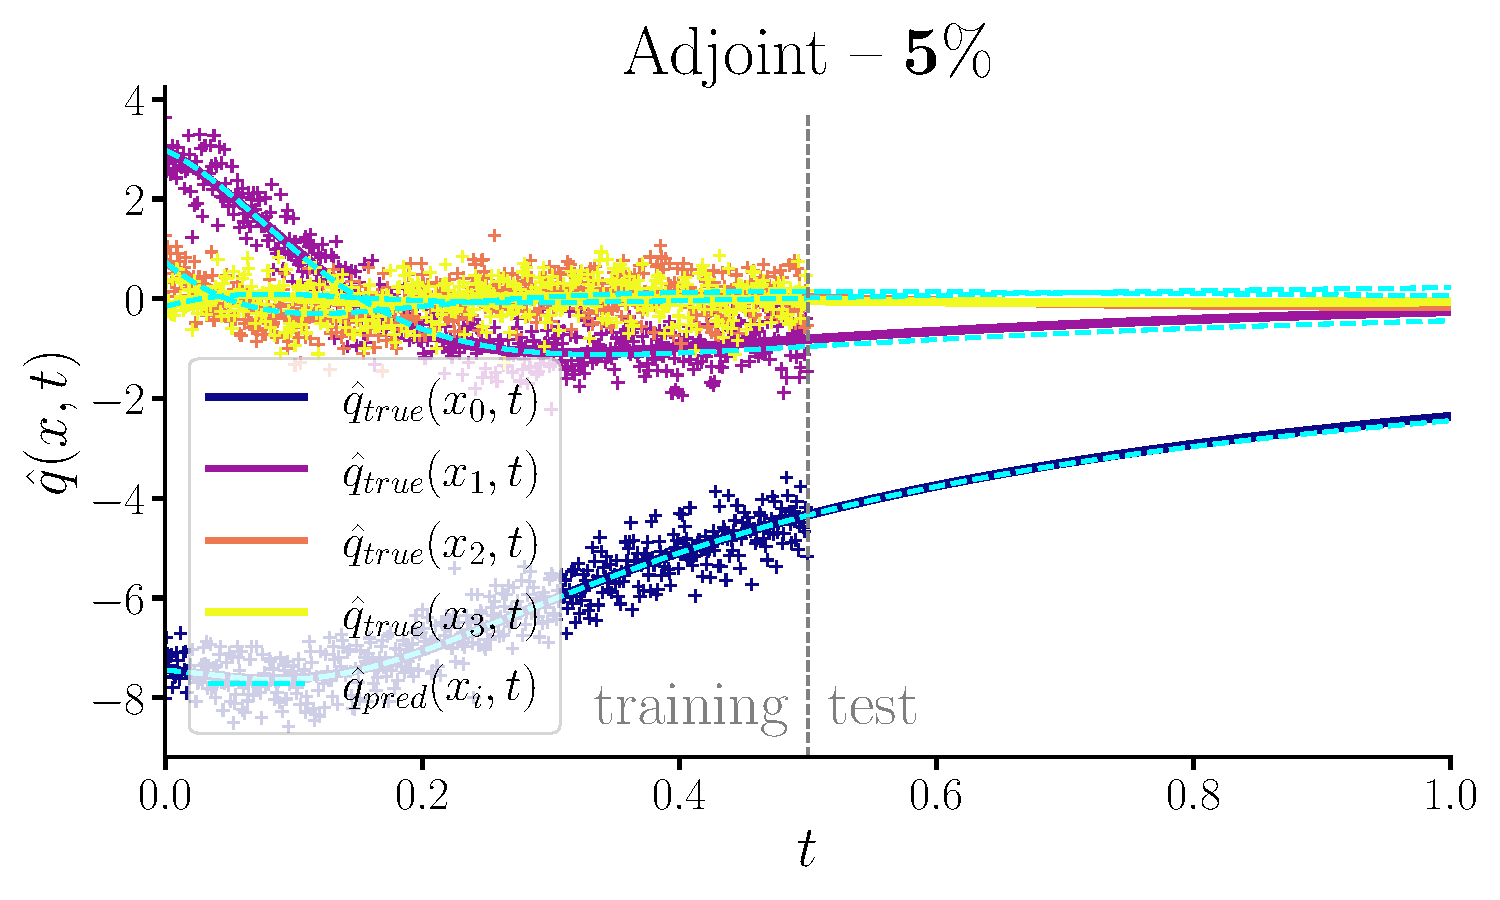
\includegraphics[width=\linewidth]{rom_noise_5_Adj.pdf}
  \end{subfigure} \\[1ex]
    
  \begin{subfigure}[c]{0.49\textwidth}
      \centering
      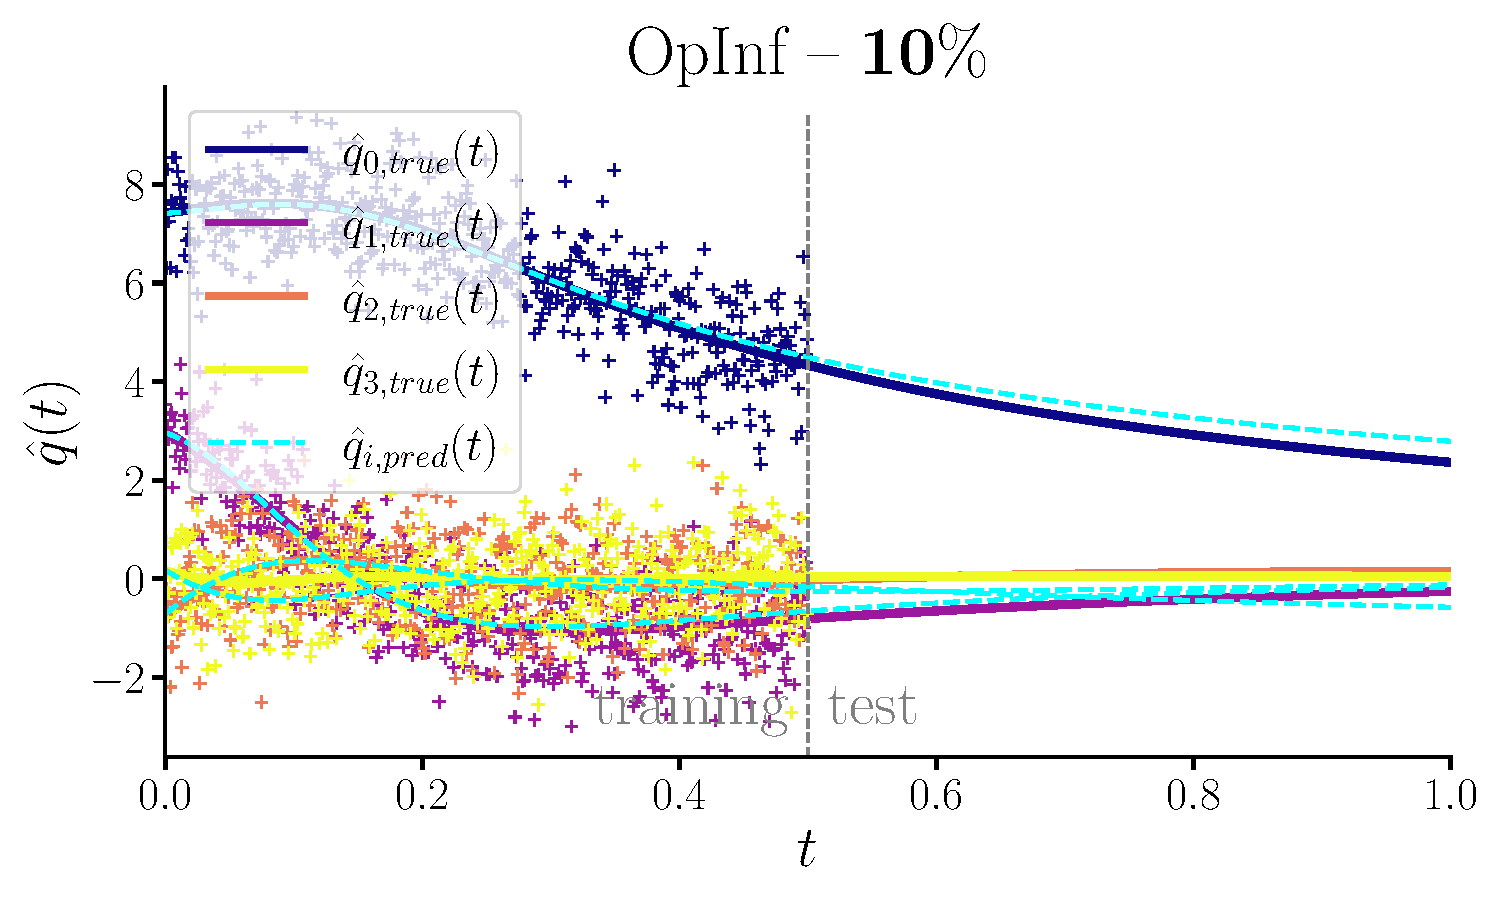
\includegraphics[width=\linewidth]{rom_noise_10_OpInf.pdf}
  \end{subfigure} 
  \begin{subfigure}[c]{0.49\textwidth}
      \centering
      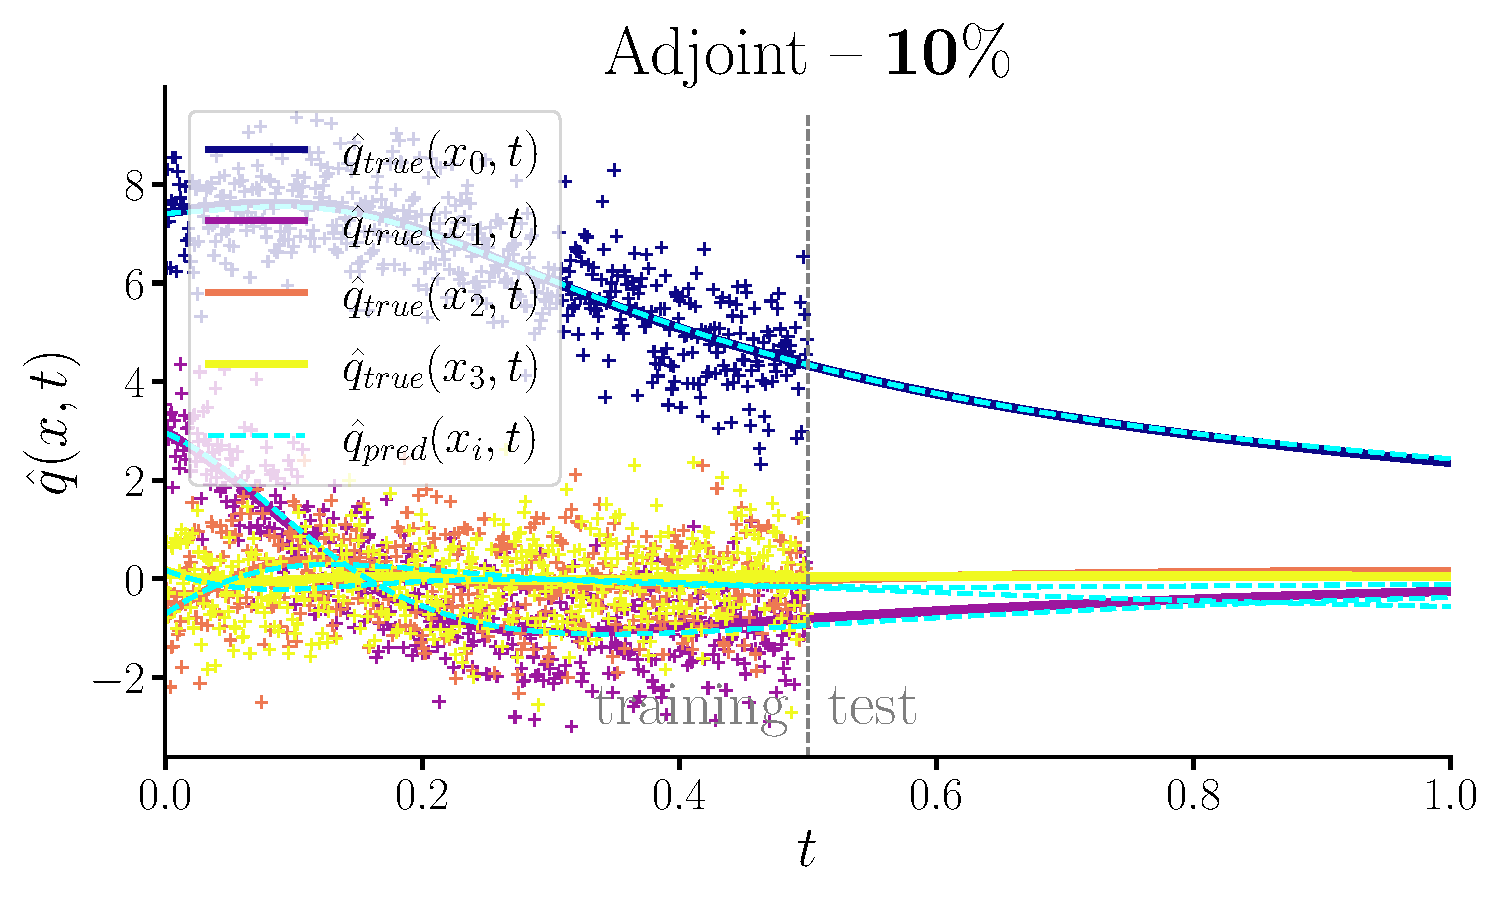
\includegraphics[width=\linewidth]{rom_noise_10_Adj.pdf}
  \end{subfigure} \\[1ex]
    
  \begin{subfigure}[c]{0.49\textwidth}
      \centering
      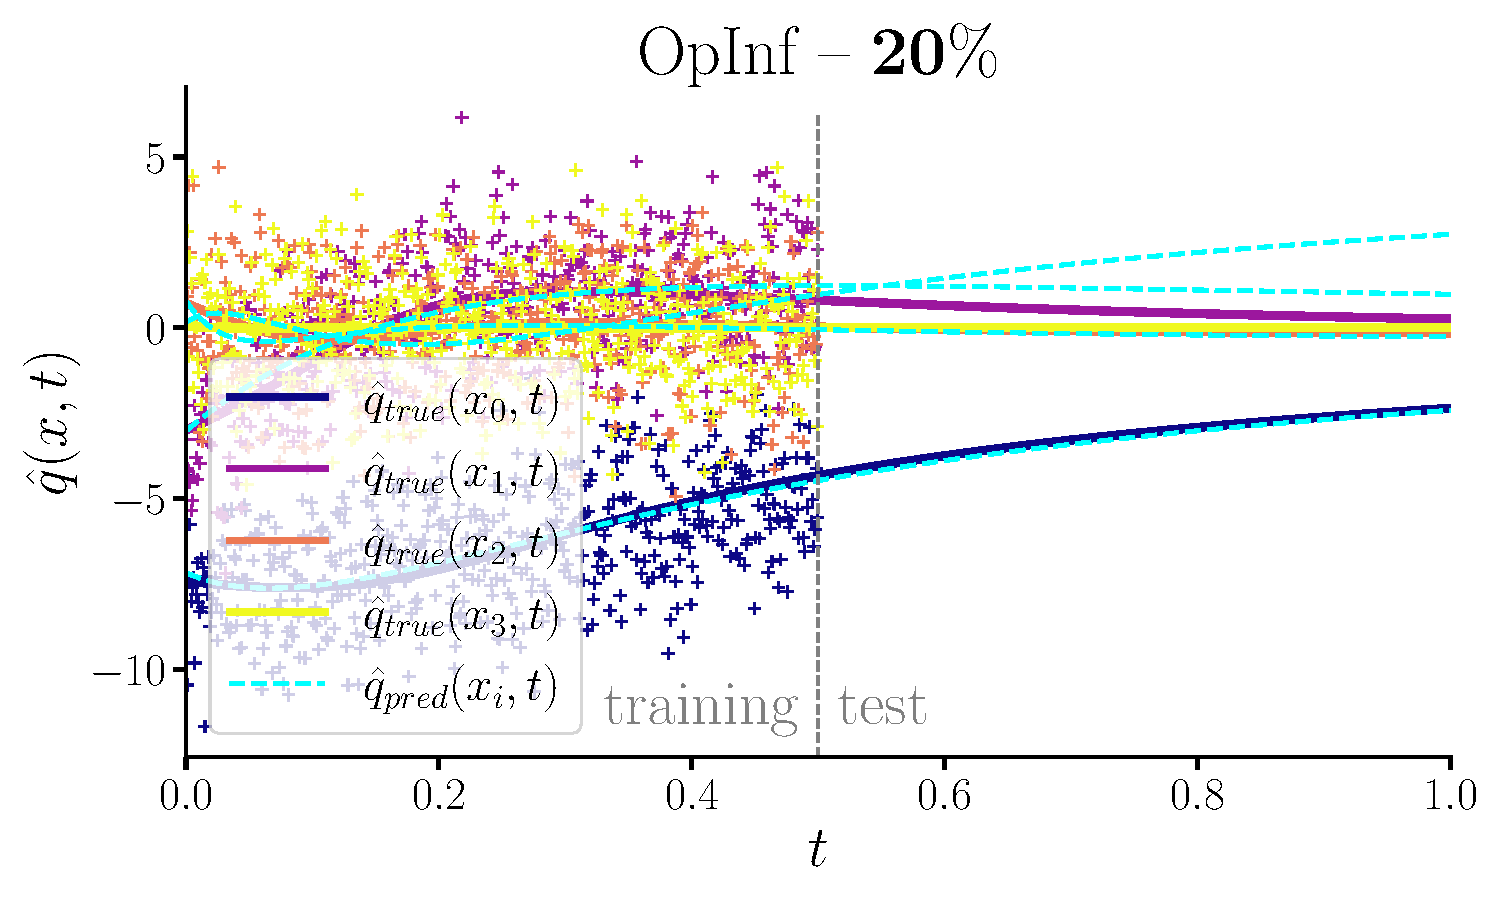
\includegraphics[width=\linewidth]{rom_noise_20_OpInf.pdf}
  \end{subfigure} 
  \begin{subfigure}[c]{0.49\textwidth}
      \centering
      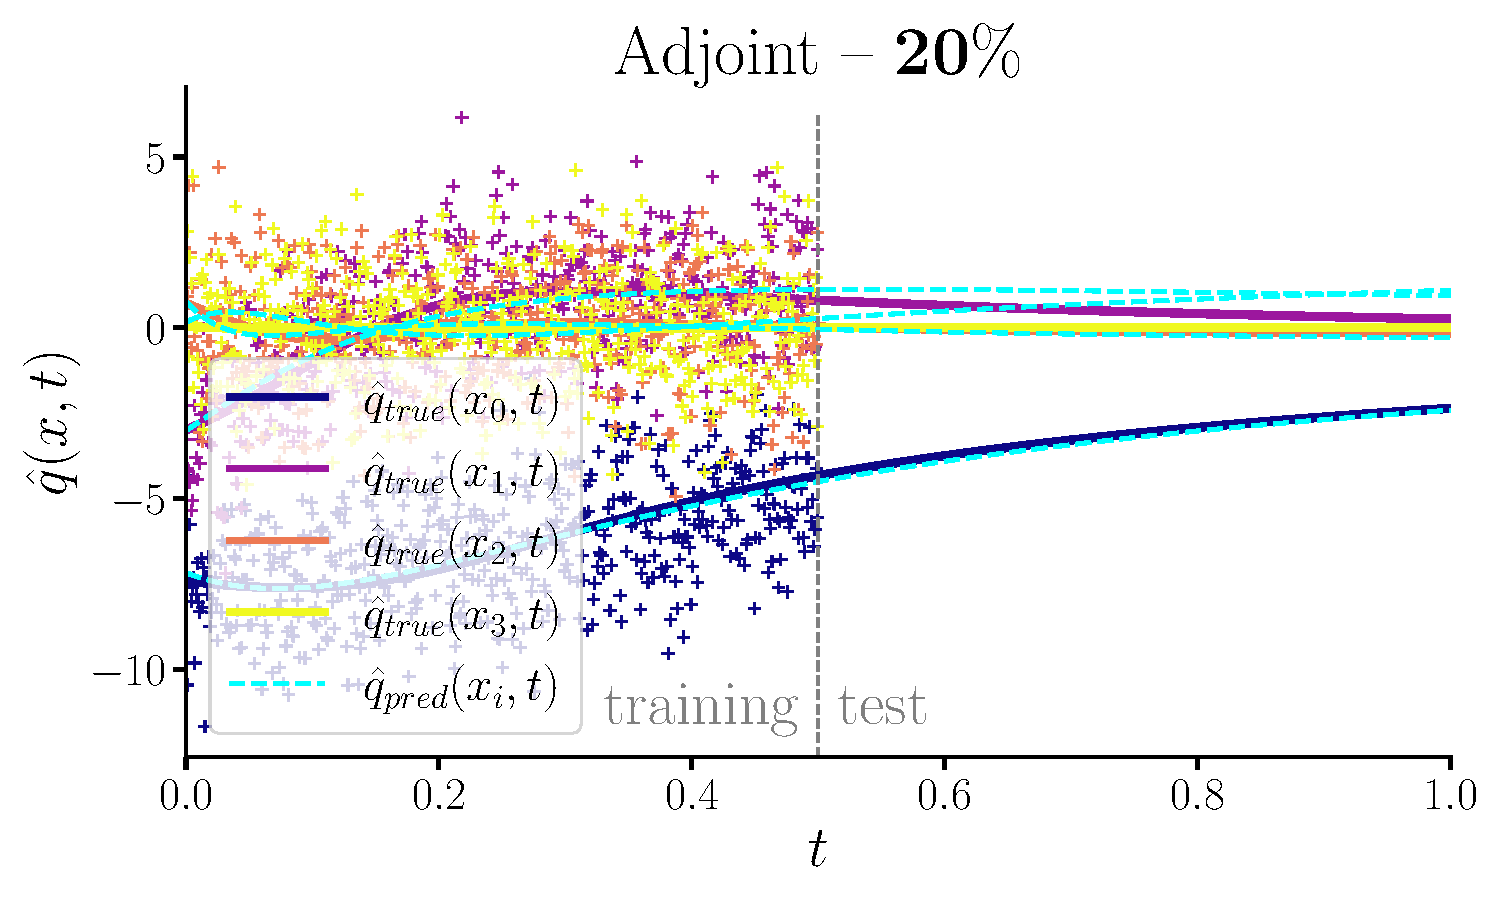
\includegraphics[width=\linewidth]{rom_noise_20_Adj.pdf}
  \end{subfigure} \\[1ex]
  \caption{Noise perturbation simulations for the Burgers' Equation synthetic experiment.}
  \label{fig:five_by_two3}
\end{figure}

\newpage

To assess robustness under imperfect data, we corrupt the full-order snapshots with additive Gaussian noise.  Specifically, we draw\\
$$\mathrm{error} \sim \mathcal{N}\bigl(0,\sigma^2\bigr),
\quad \sigma = \|\mathbf{q}\|_{\mathrm{max}}\,\frac{\text{pct}}{100},$$ 
for noise levels of 1\%, 5\%, 10\%, and 20\%.  Each noisy dataset is then used to train both the OpInf and adjoint models over $t\in[0,0.5]$, with predictions made on $[0.5,1]$. Figure~\ref{fig:five_by_two3} visualizes the true reduced states (scatter and solid) against the trained predictions (dashed) for both methods at each noise level. As noise increases, the adjoint-trained ROM consistently tracks true trajectories more accurately than OpInf, highlighting its superior gradient fidelity in the presence of data corruption.

%%%%%% Prediction Error vs. Time (noise - Burgers) %%%%%%

Figure~\ref{fig:twobytwo3} shows the time-dependent prediction error, as previously defined, for each noise level. While all methods degrade as noise grows, the adjoint method maintains lower errors than both OpInf approaches over time.

\vspace{0.7cm}

\begin{figure}[h!]
  \centering
  
  % First row of subfigures
  \begin{subfigure}[b]{0.48\textwidth}
    \centering
    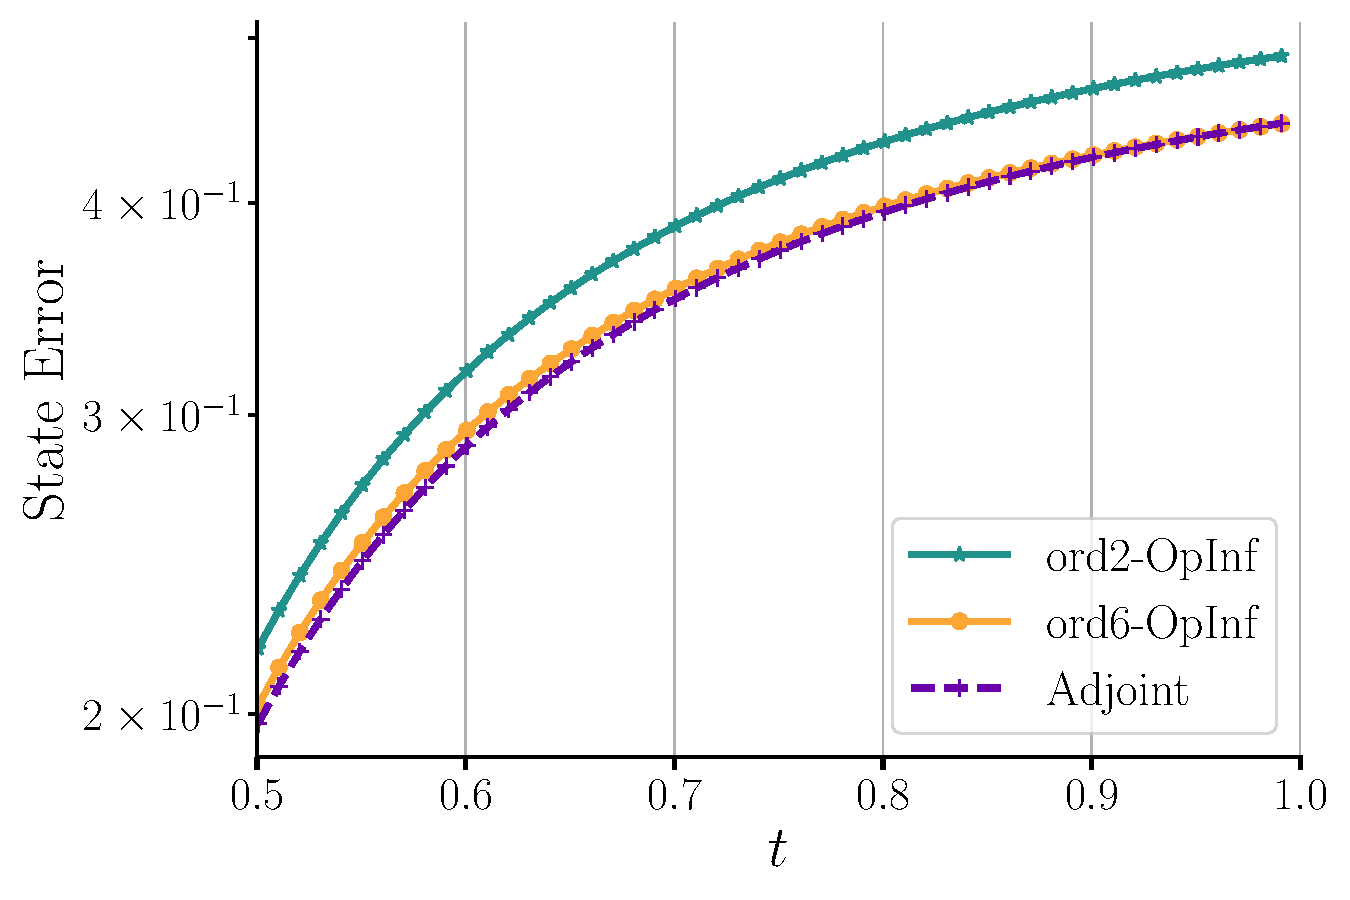
\includegraphics[width=\linewidth]{pred_error_vs_time_noise_1.pdf}
    \caption{1\% of noise level.}
    \label{fig:image1}
  \end{subfigure}
  \quad
  \begin{subfigure}[b]{0.48\textwidth}
    \centering
    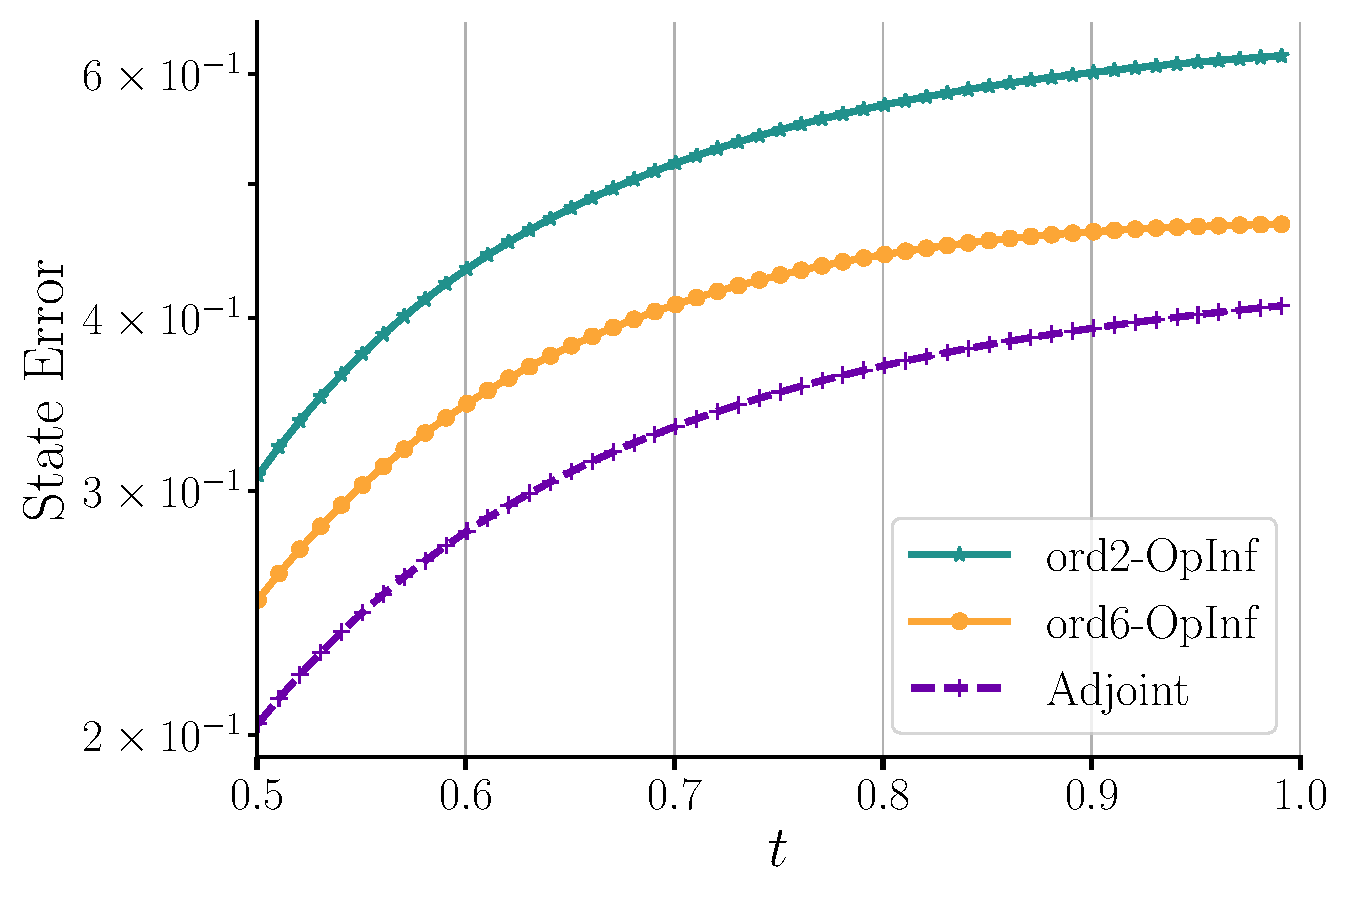
\includegraphics[width=\linewidth]{pred_error_vs_time_noise_5.pdf}
    \caption{5\% of noise level.}
    \label{fig:image2}
  \end{subfigure}
  
  \vskip\baselineskip
  
  % Second row of subfigures
  \begin{subfigure}[b]{0.48\textwidth}
    \centering
    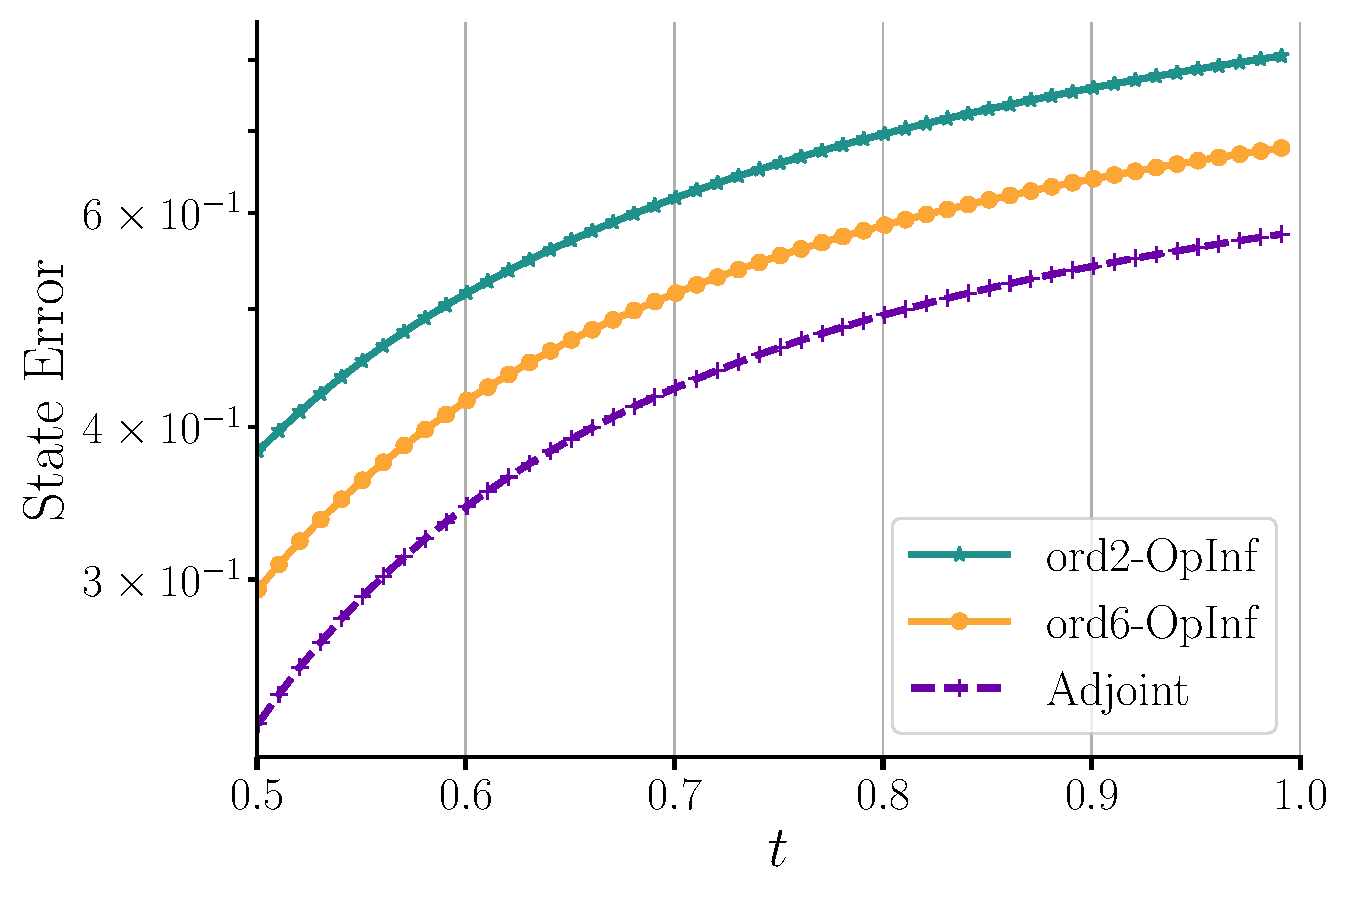
\includegraphics[width=\linewidth]{pred_error_vs_time_noise_10.pdf}
    \caption{10\% of noise level.}
    \label{fig:image3}
  \end{subfigure}
  \quad
  \begin{subfigure}[b]{0.48\textwidth}
    \centering
    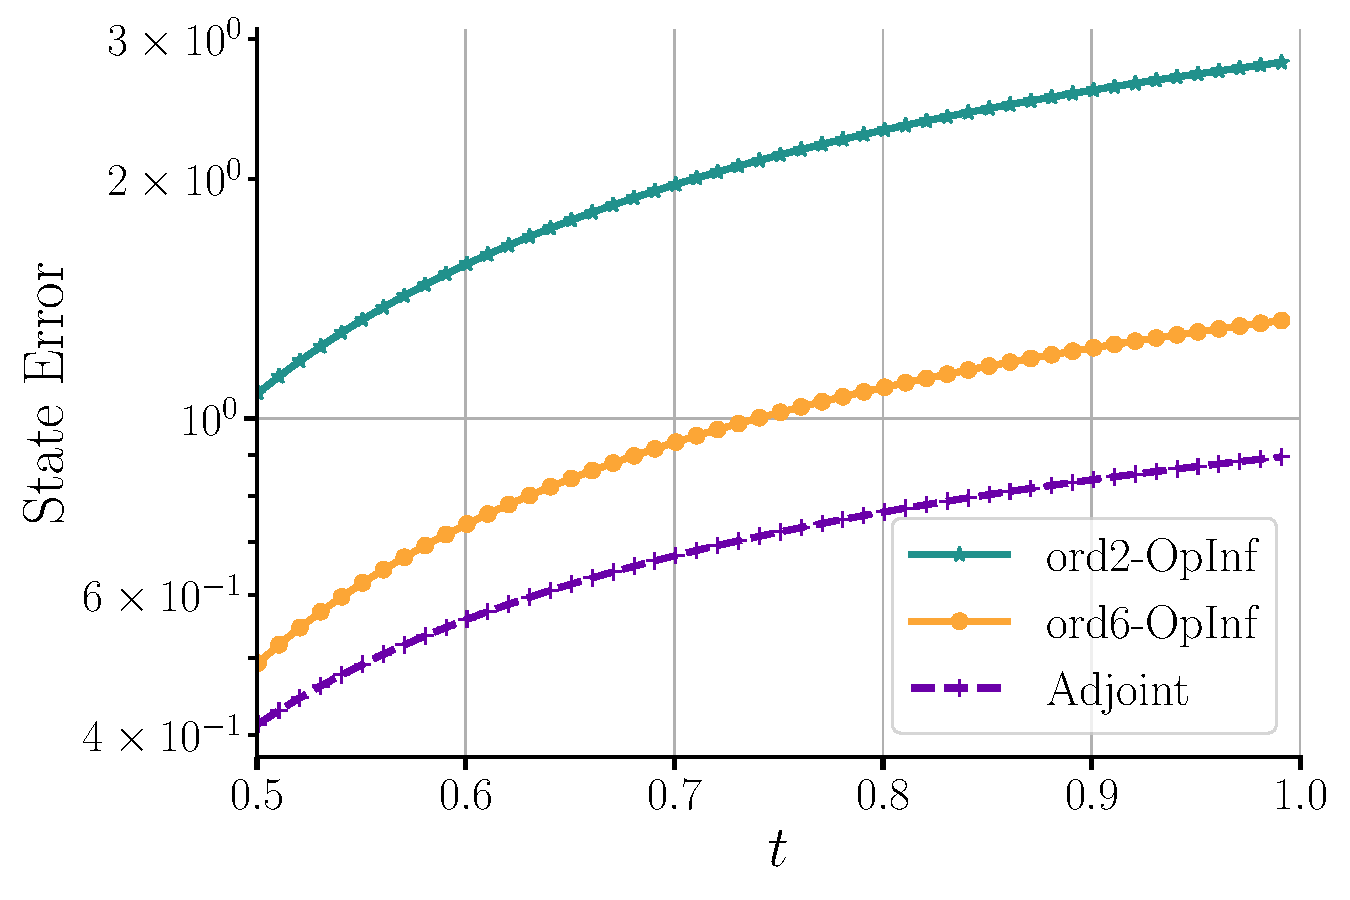
\includegraphics[width=\linewidth]{pred_error_vs_time_noise_20.pdf}
    \caption{20\% of noise level.}
    \label{fig:image4}
  \end{subfigure}
  
  \caption{Prediction error vs. time for each noise level run in the Burgers' Equation experiment.}
  \label{fig:twobytwo3}
\end{figure}

\newpage

%%%%%% Relative Error vs. r (noise - Burgers)%%%%%%

To further quantify model efficiency, Figure~\ref{fig:twobytwo4} plots the relative error as a function of the model dimension $r$. For each noise level, we observe that the adjoint-trained ROM achieves a better accuracy for the same number of modes than both OpInf methods, especially at 5\%, 10\% and 20\% noise.  This confirms that the adjoint gradient yields more informative parameter updates even when training data are corrupted.

\vspace{0.7cm}

\begin{figure}[h!]
  \centering
  
  % First row of subfigures
  \begin{subfigure}[b]{0.48\textwidth}
    \centering
    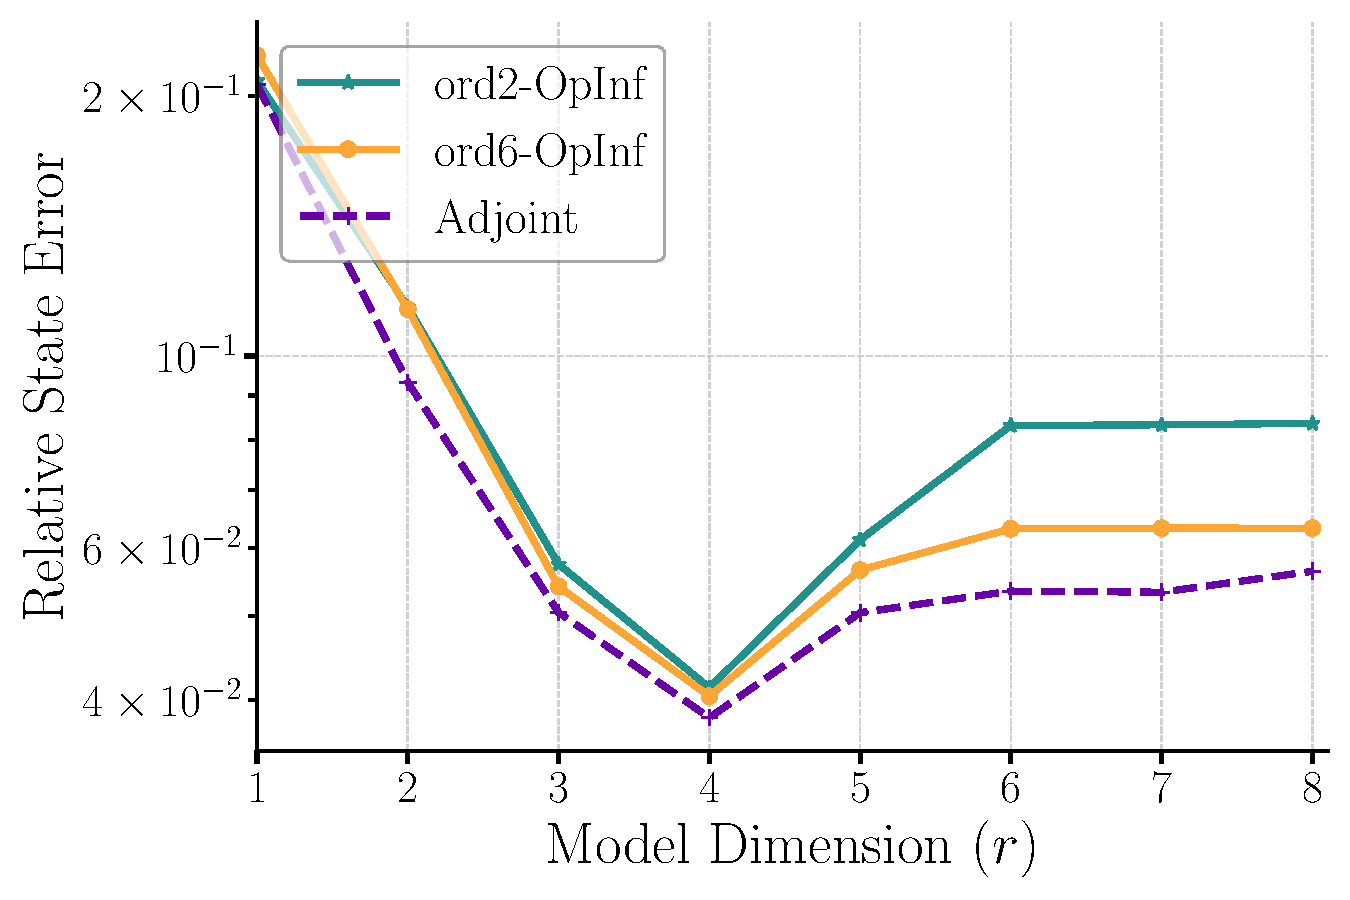
\includegraphics[width=\linewidth]{rel_error_vs_r_noise_1.pdf}
    \caption{1\% of noise level.}
    \label{fig:image1}
  \end{subfigure}
  \quad
  \begin{subfigure}[b]{0.48\textwidth}
    \centering
    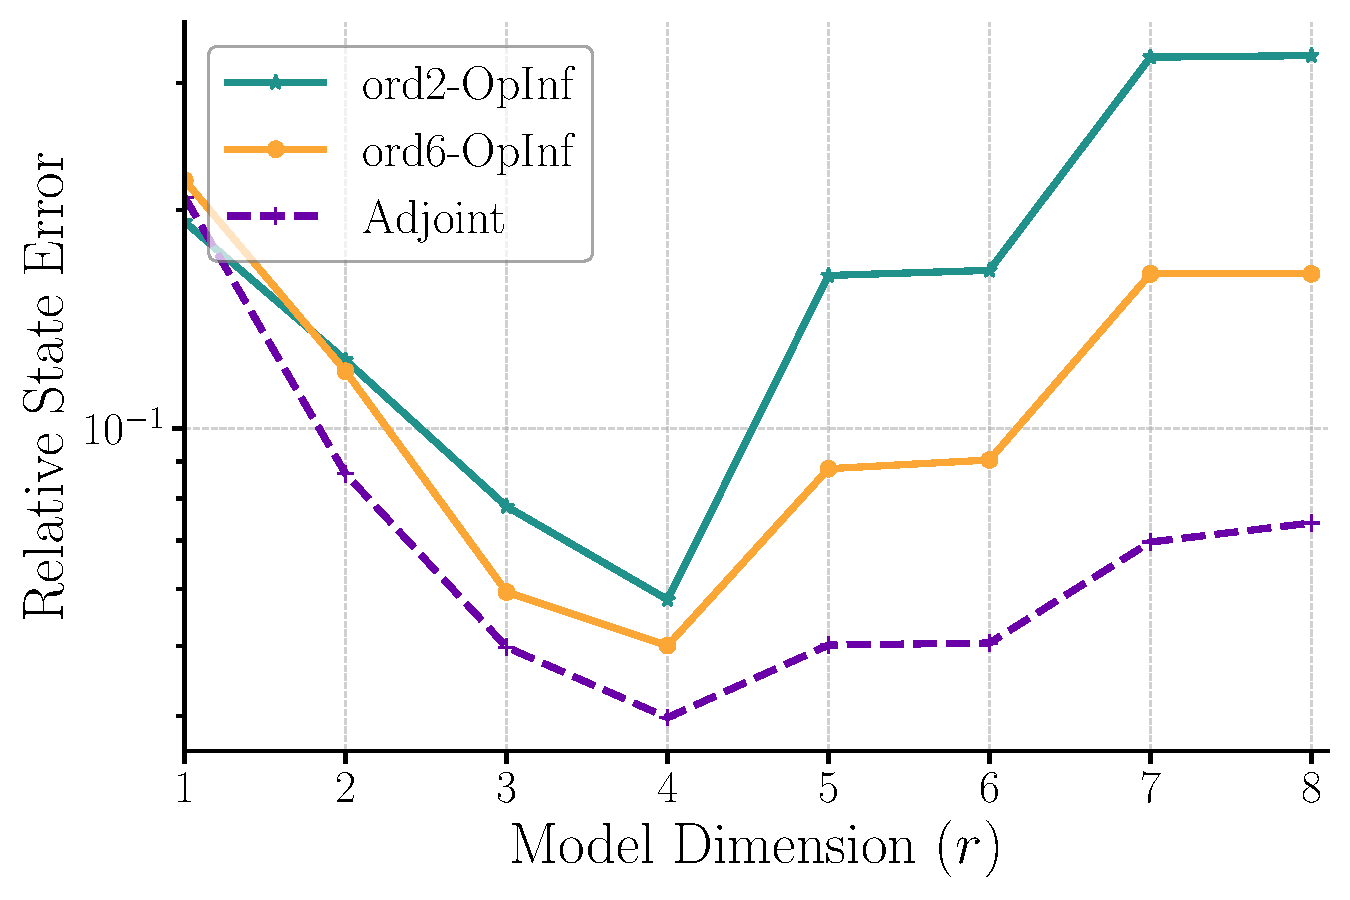
\includegraphics[width=\linewidth]{rel_error_vs_r_noise_5.pdf}
    \caption{5\% of noise level.}
    \label{fig:image2}
  \end{subfigure}
  
  \vskip\baselineskip
  
  % Second row of subfigures
  \begin{subfigure}[b]{0.48\textwidth}
    \centering
    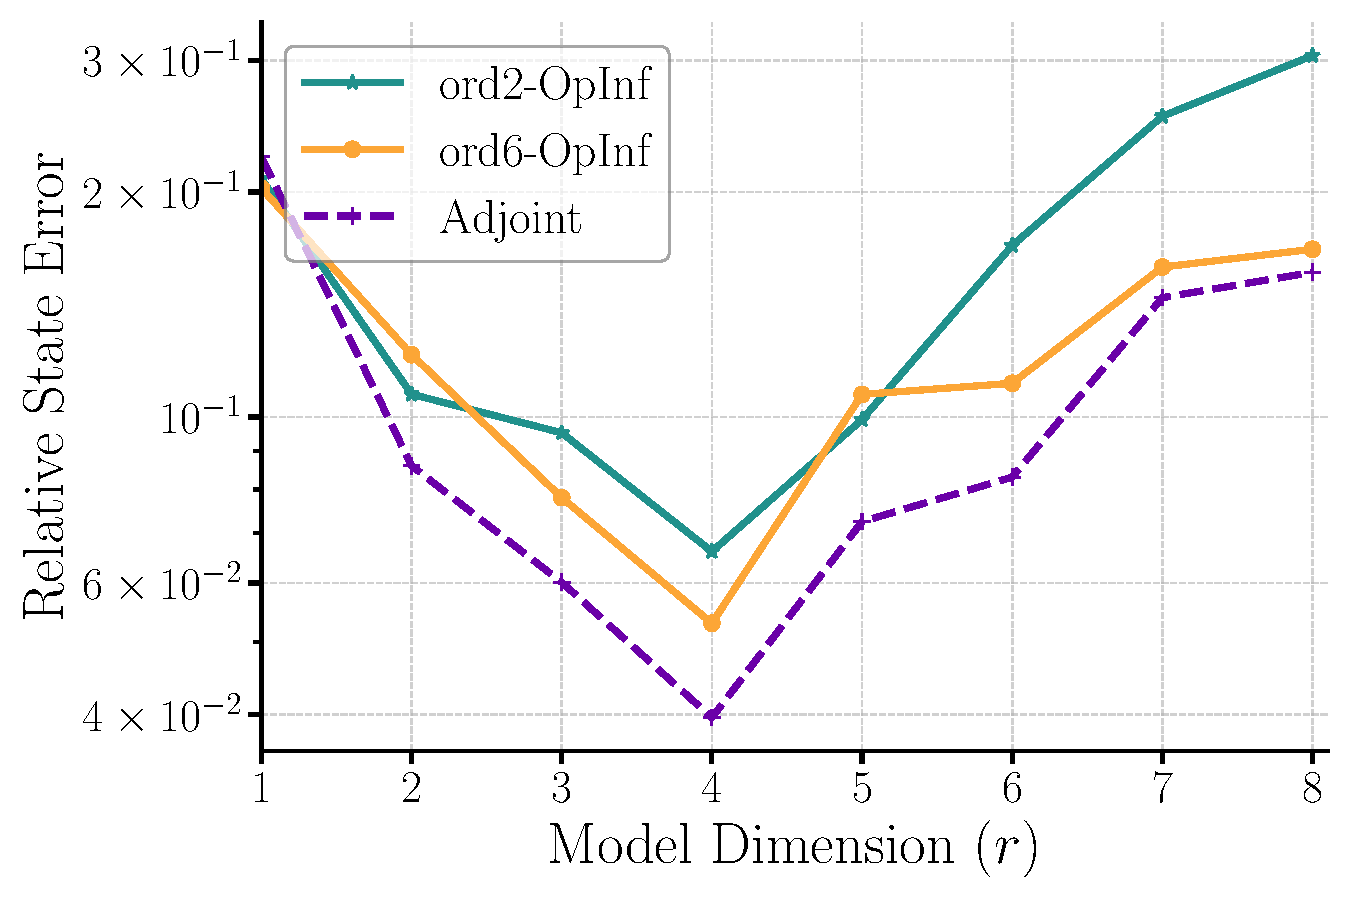
\includegraphics[width=\linewidth]{rel_error_vs_r_noise_10.pdf}
    \caption{10\% of noise level.}
    \label{fig:image3}
  \end{subfigure}
  \quad
  \begin{subfigure}[b]{0.48\textwidth}
    \centering
    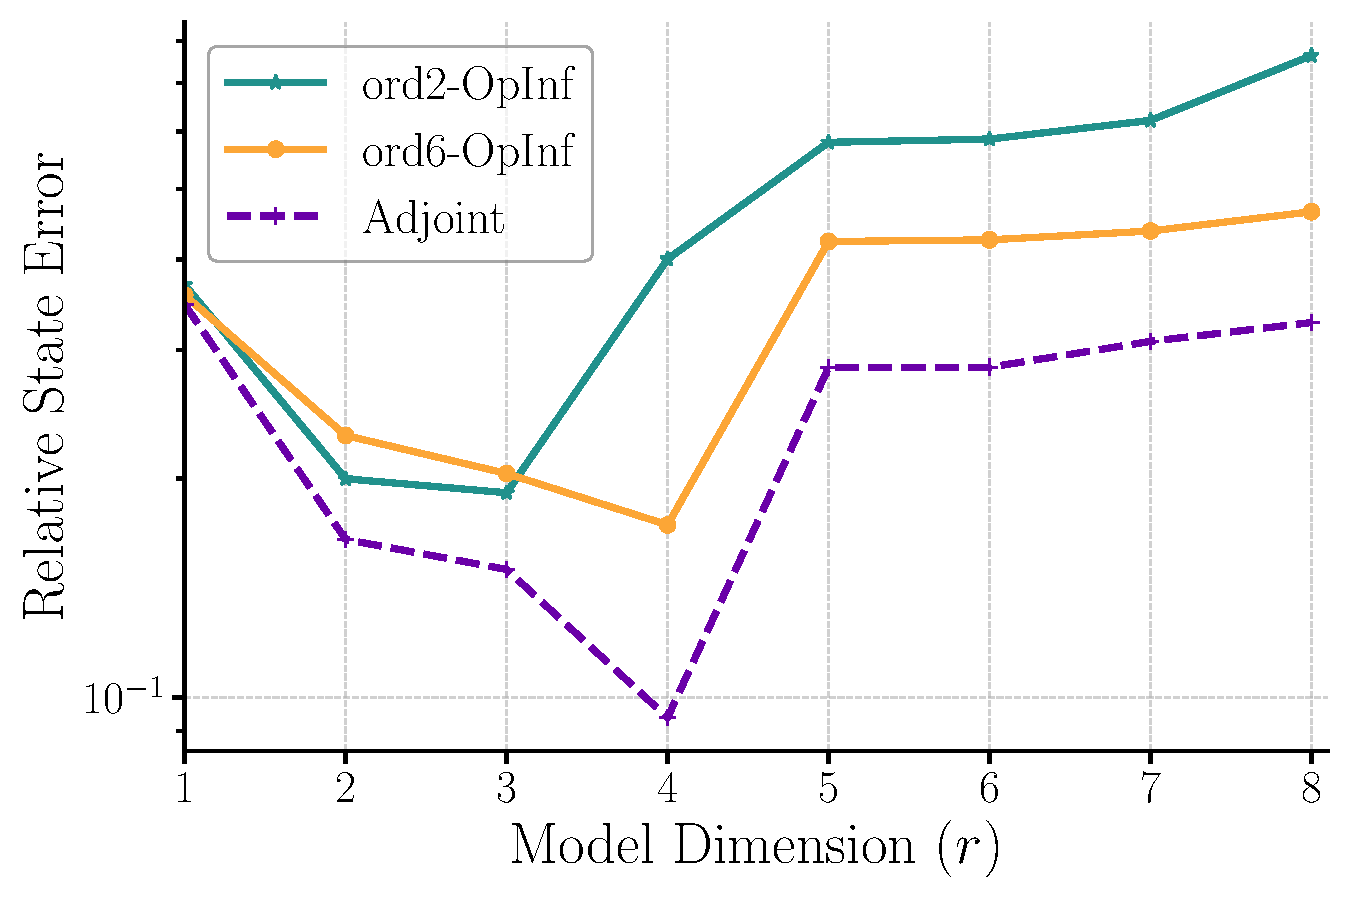
\includegraphics[width=\linewidth]{rel_error_vs_r_noise_20.pdf}
    \caption{20\% of noise level.}
    \label{fig:image4}
  \end{subfigure}
  
  \caption{Relative error vs. $r$ for each noise perturbation run in the Burgers' Equation experiment.}
  \label{fig:twobytwo4}
\end{figure}

\newpage

%%%%%%%%%%%%%%%%%%%%%%%%%%%%%%%%%%%%%%%%%%%%%%%%%%%%%%%%%%%%%%%%%%%%%%%%%%%%%%%%%%%%%%%%%%%%%%
%%%%%%%%%%%%%%%%%%%%%%%%%%%%%%%%%%%%%%%%% FKPP EQUATION %%%%%%%%%%%%%%%%%%%%%%%%%%%%%%%%%%%%%%
%%%%%%%%%%%%%%%%%%%%%%%%%%%%%%%%%%%%%%%%%%%%%%%%%%%%%%%%%%%%%%%%%%%%%%%%%%%%%%%%%%%%%%%%%%%%%%

\section{Fisher-KPP Equation}
\label{sec:fkpp_eq}

\subsection*{Snapshot Data Generation}

For this second synthetic experiment, we generate training data (see code in Appendix \ref{lst:fkpp}) by numerically solving the two-dimensional Fisher-KPP equation,\\
$$q_t = \mathfrak{D}\,(q_{xx} + q_{yy}) \;+\; \rho\,q\,(1 - q), \quad (x,y)\in[0,L_x]\times[0,L_y],\;t\in[0,T],$$
with homogeneous Neumann (zero-flux) boundary conditions\\
$$\frac{\partial q}{\partial n}\Big|_{\partial\Omega} = 0,$$
and a Gaussian initial condition centered in the domain:\\
$$q(x,y,0)= \exp\Bigl(-10\bigl[(x - L_x/2)^2 + (y - L_y/2)^2\bigr]\Bigr).$$

The following parameters and grid are considered:
\begin{itemize}
  \item Domain sizes: $L_x = L_y = 10$.
  \item Grid: $N_x = N_y = 100$ points in each direction, $\Delta x = L_x/(N_x-1)$, $\Delta y = L_y/(N_y-1)$.
  \item Time stepping: final time $T=5$, $\Delta t=0.005$, $N_t = T/\Delta t = 1000$.
  \item Model parameters: diffusion coefficient $\mathfrak{D}=0.1$, logistic growth rate $\rho=1.0$.
\end{itemize}
A finite difference method is then applied for the spatial discretizations:
\begin{itemize}
  \item For the $x$-dimension, we construct a 1D second-difference matrix $\mathbf{L}_x^{1D}\in\mathbb R^{N_x\times N_x}$ with Neumann BCs by\\
$$\bigl(\mathbf{L}_x^{1D}\bigr)_{jj}= -\frac{2}{\Delta x^2}, \quad \bigl(\mathbf{L}_x^{1D}\bigr)_{j,j\pm1}= \frac{1}{\Delta x^2},
      \quad (\mathbf{L}_x^{1D})_{0,1} = (\mathbf{L}_x^{1D})_{N_x-1,N_x-2} = \frac{2}{\Delta x^2}.$$
  \item Similarly, we define \(\mathbf{L}_y^{1D}\in\mathbb R^{N_y\times N_y}\) on the \(y\)-grid.
  \item Both expressions are combined to form a full 2D-Laplacian by Kronecker sums\\
    $$\mathbf{L} = \mathbf{I}_{N_y}\otimes \mathbf{L}_x^{1D} \;+\; \mathbf{L}_y^{1D}\otimes \mathbf{I}_{N_x}\quad\in\mathbb R^{(N_xN_y)\times(N_xN_y)}.$$
\end{itemize}
For the time-stepping scheme, we use a semi-implicit Crank-Nicolson step for the diffusion and explicit Euler for the reaction term:\\
$$\dfrac{\mathbf{q}^{m+1} - \mathbf{q}^{m}}{\Delta t} = \dfrac{\mathfrak{D}}{2}\mathbf{L}(\mathbf{q}^{m+1}+\mathbf{q}^m)\;+\,\rho\,\mathbf{q}^m\circ(\mathbf{1} - \mathbf{q}^m),$$ 
where "$\circ$" denotes the Hadamard product.

By defining,
$$\alpha \;\coloneqq\;\frac{\mathfrak{D}\,\Delta t}{2}, \quad \bm{\mathcal{A}} \;\coloneqq\; \mathbf{I} - \alpha\,\mathbf{L}, \quad \bm{\mathcal{B}} \;\coloneqq\; \mathbf{I} + \alpha\,\mathbf{L},$$
then at each time step\\
$$\bm{\mathcal{A}}\mathbf{q}^{m+1} = \bm{\mathcal{B}}\mathbf{q}^m + \Delta t\,\rho\,\mathbf{q}^m\circ(\mathbf{1} - \mathbf{q}^m).$$
By solving this sparse linear system we get the desired state solution at every time step that we will use to build the snapshot matrix
$\mathbf{Q}\in\mathbb R^{(N_xN_y)\times N_t}.$

Visualization of the dynamics for the Fisher-KPP equation is shown in Figure~\ref{fig:fisher-data}.

\begin{figure}[h!]
    \hspace{-0.8cm}
  \centering
  \begin{subfigure}[t]{\textwidth}
    \centering
    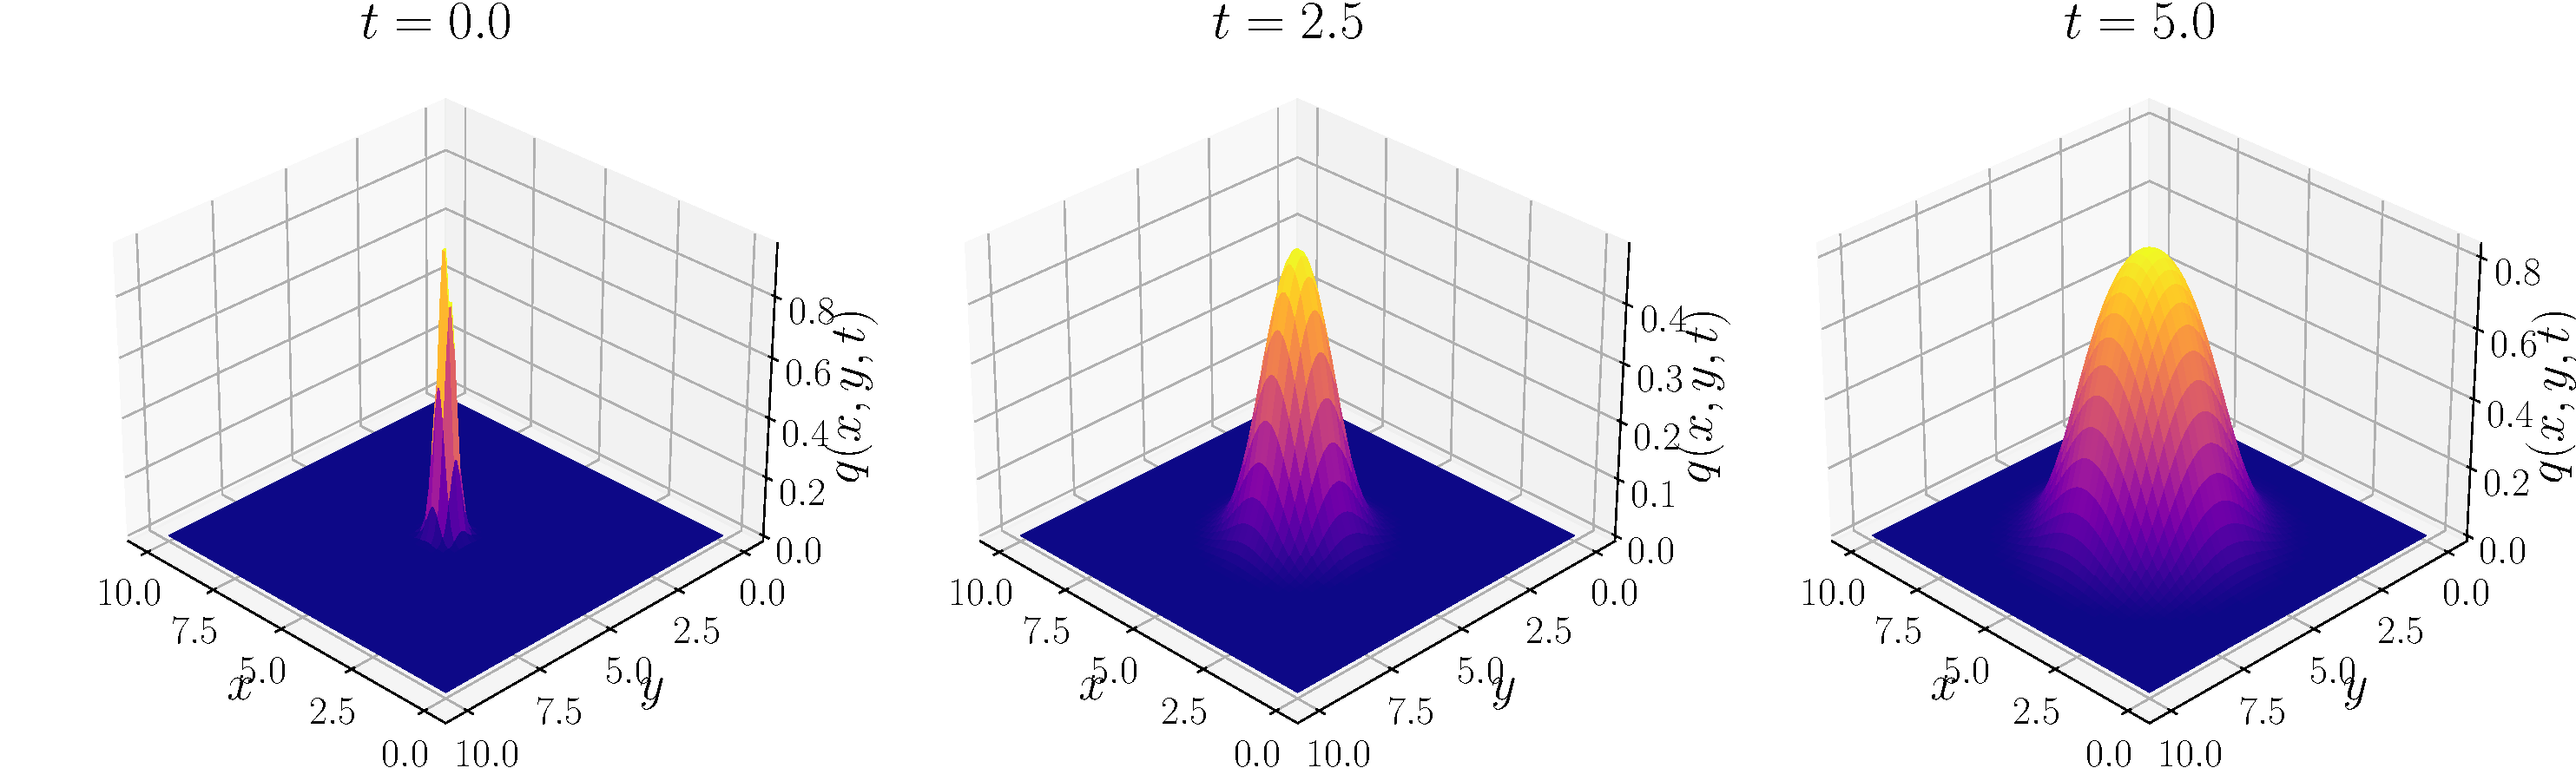
\includegraphics[width=\textwidth]{3Dfkpp.pdf}
    \caption{3D surface of $q(x,y,t)$ for $\mathfrak{D}=0.1$ and $\rho=1$.}
    \label{fig:fisher-init}
  \end{subfigure}
  \\[1em]
  \begin{subfigure}[t]{0.48\textwidth}
    \centering
    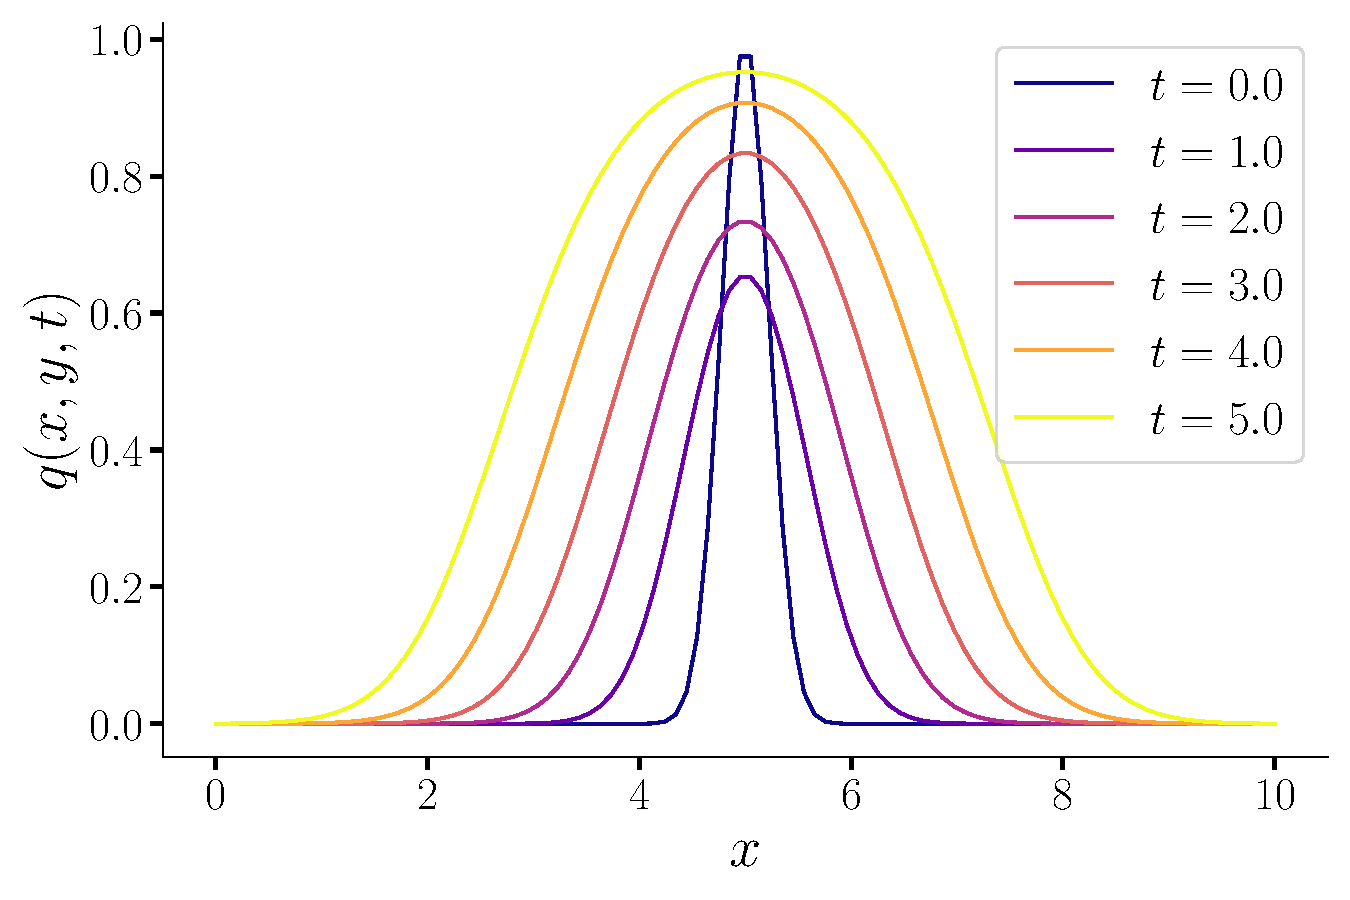
\includegraphics[width=\textwidth]{1Dfkpp.pdf}
    \caption{Profiles of $q(x.y.t)$ for different $t_k$.}
    \label{fig:fisher-mid}
  \end{subfigure}
  \hfill
  \begin{subfigure}[t]{0.48\textwidth}
    \centering
    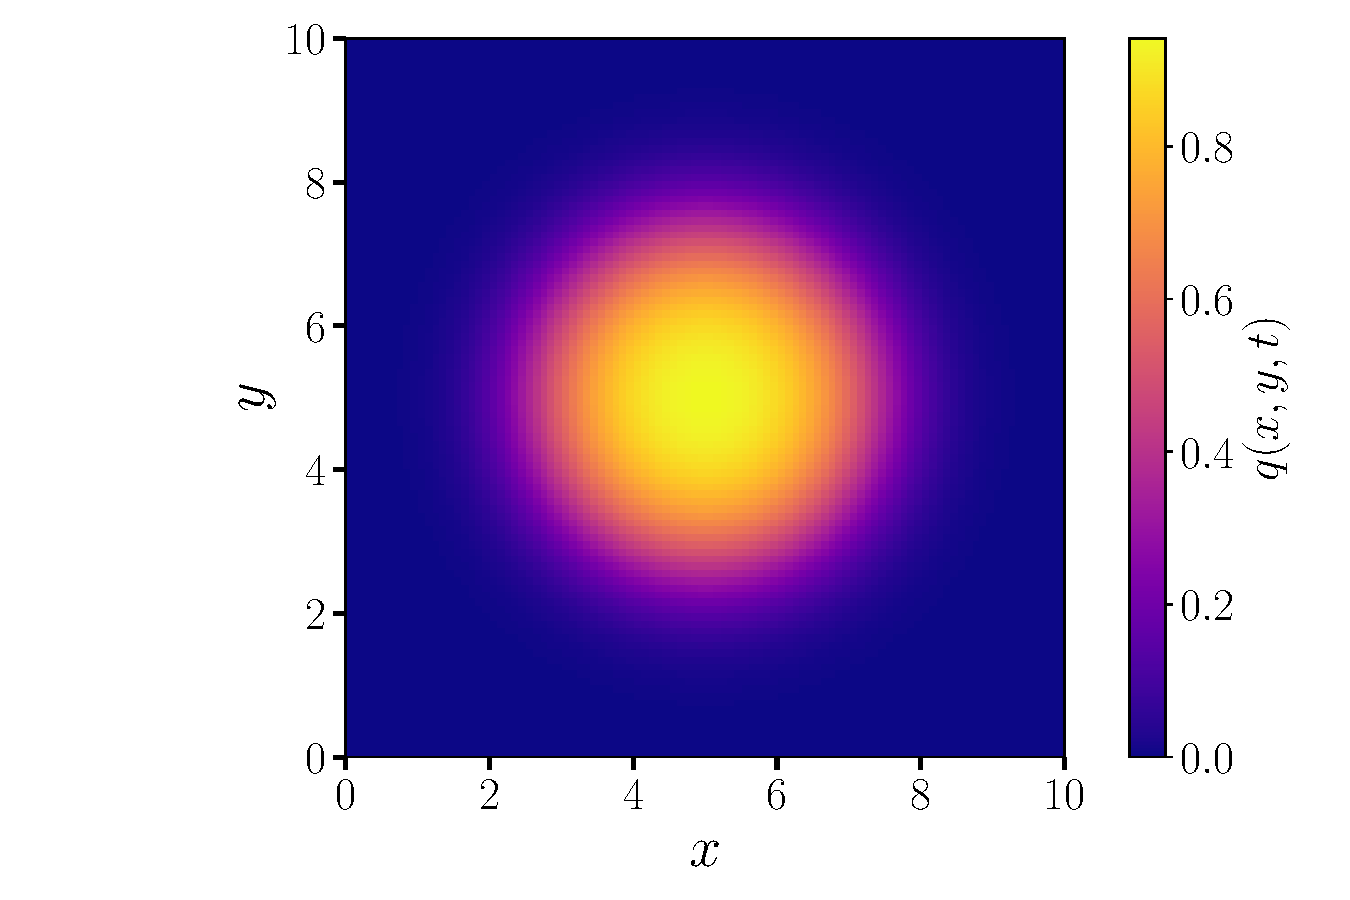
\includegraphics[width=\textwidth]{2Dfkpp.pdf}
    \caption{Space-time contour of $q(x,y,t)$ at $t=5$.}
    \label{fig:fisher-final}
  \end{subfigure}
  \caption{Dynamics of the FKPP equation used for data generation.}
  \label{fig:fisher-data}
\end{figure}     

\newpage

%%%%%%%%%%%%%%%%%%%%%%%%%%%%%%%%% NOISE PERTURBATION %%%%%%%%%%%%%%%%%%%%%%%%%%%%%%%%%%

\subsection*{Noise Perturbation}

\vspace{1.0cm}

\begin{figure}[h!]
  \centering
  \begin{subfigure}[c]{0.49\textwidth}
      \centering
      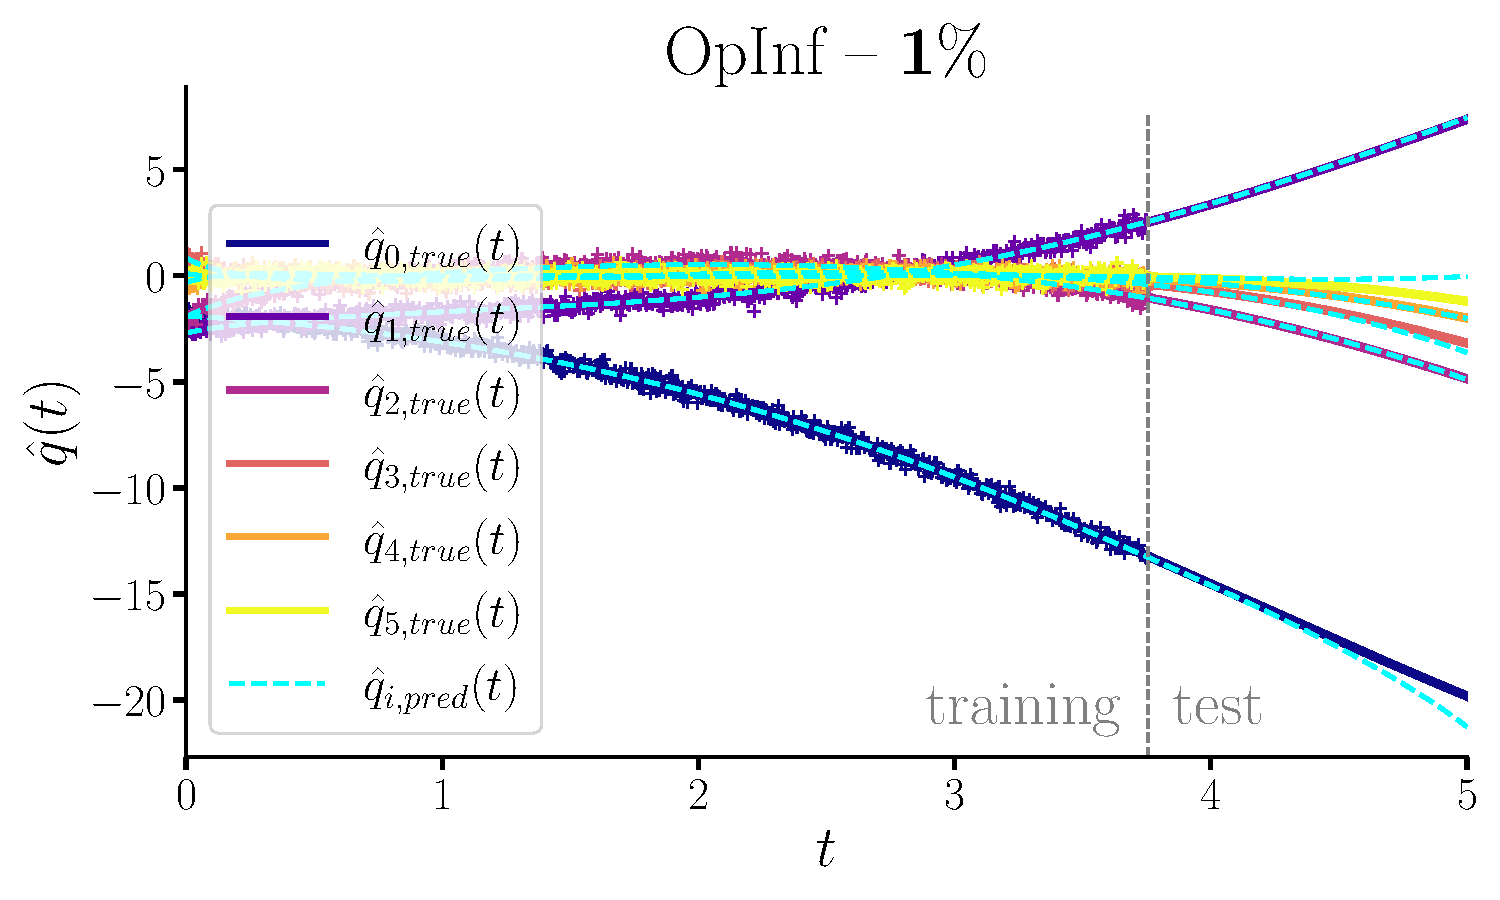
\includegraphics[width=\linewidth]{fkpp_rom_noise_1_OpInf.pdf}
  \end{subfigure}
  \begin{subfigure}[c]{0.49\textwidth}
      \centering
      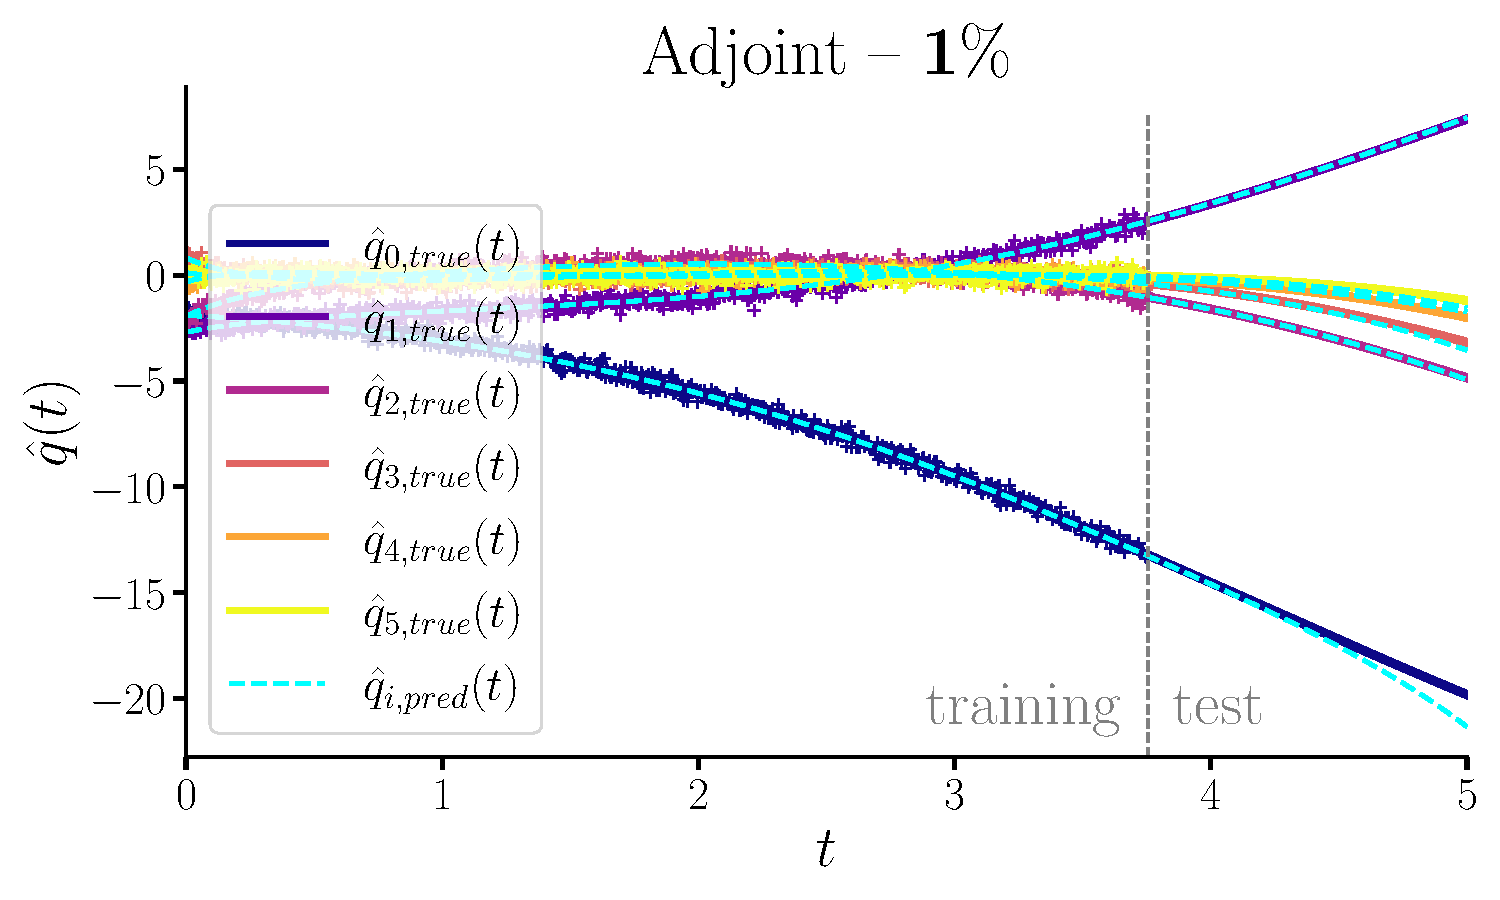
\includegraphics[width=\linewidth]{fkpp_rom_noise_1_Adj.pdf}
  \end{subfigure} \\[1ex]
    
  \begin{subfigure}[c]{0.49\textwidth}
      \centering
      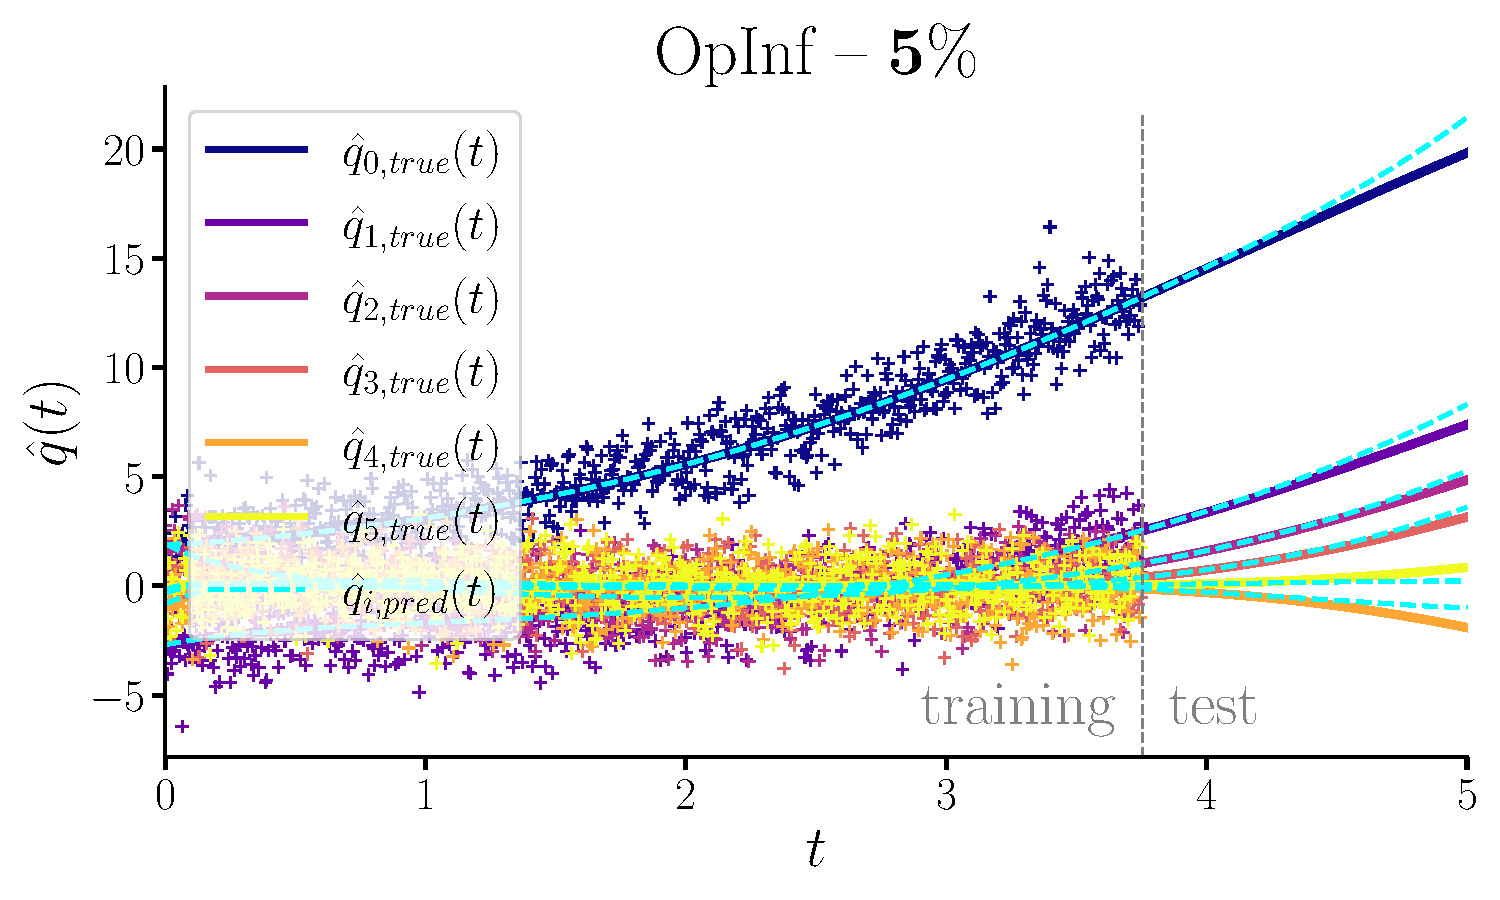
\includegraphics[width=\linewidth]{fkpp_rom_noise_5_OpInf.pdf}
  \end{subfigure} 
  \begin{subfigure}[c]{0.49\textwidth}
      \centering
      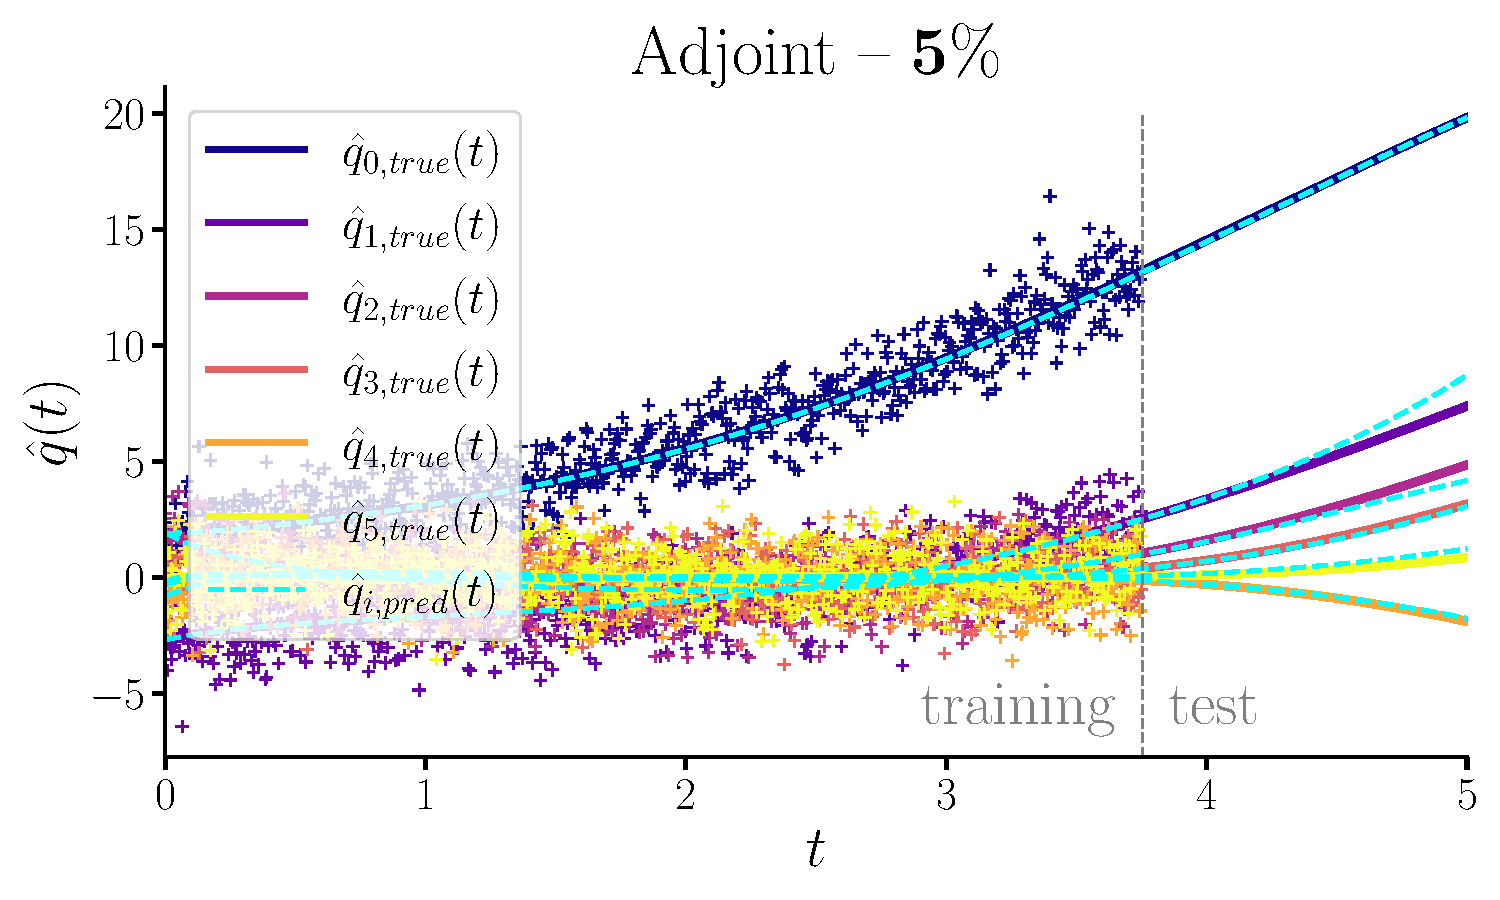
\includegraphics[width=\linewidth]{fkpp_rom_noise_5_Adj.pdf}
  \end{subfigure} \\[1ex]
    
  \begin{subfigure}[c]{0.49\textwidth}
      \centering
      \includegraphics[width=\linewidth]{fkpp_rom_noise_10_OpInf.pdf}
  \end{subfigure} 
  \begin{subfigure}[c]{0.49\textwidth}
      \centering
      \includegraphics[width=\linewidth]{fkpp_rom_noise_10_Adj.pdf}
  \end{subfigure} \\[1ex]
    
  \begin{subfigure}[c]{0.49\textwidth}
      \centering
      \includegraphics[width=\linewidth]{fkpp_rom_noise_20_OpInf.pdf}
  \end{subfigure} 
  \begin{subfigure}[c]{0.49\textwidth}
      \centering
      \includegraphics[width=\linewidth]{fkpp_rom_noise_20_Adj.pdf}
  \end{subfigure} \\[1ex]
  \caption{Noise perturbation simulations for the FKPP Equation synthetic experiment.}
  \label{fig:five_by_two4}
\end{figure}

\newpage

%Global summary for FKPP noise experiments%

In the case of the 2D Fisher-KPP equation, we omit the data density reduction study since it yielded virtually the same conclusions as for Burgers' with no significant performance gap between sixth-order OpInf and the adjoint method. Instead, we focus solely on the noise perturbation results, which are displayed in Figures~\ref{fig:five_by_two4}, \ref{fig:twobytwo5}, and \ref{fig:twobytwo6}. Due to stability considerations in the reaction-diffusion dynamics, we extended in this case the training window to cover 75\% of the total simulation time.

Across all four noise levels (1\%, 5\%, 10\%, and 20\%), the adjoint-trained ROM consistently outperformed the best OpInf configuration (\texttt{'ord6'}), both in trajectory fidelity and in error metrics. 

%%%%%% Prediction Error vs. Time (noise - FKPP) %%%%%%

In the time-series comparisons of the reduced states (Figure~\ref{fig:twobytwo5}), the corresponding prediction-error curves confirm that the adjoint approach maintains lower error evolution over the prediction interval, especially at the highest noise levels, where the estimates of the finite difference derivative degrade significantly.

\vspace{0.7cm}

\begin{figure}[h!]
  \centering
  
  % First row of subfigures
  \begin{subfigure}[b]{0.48\textwidth}
    \centering
    \includegraphics[width=\linewidth]{fkpp_pred_error_vs_time_noise_1.pdf}
    \caption{1\% of noise level.}
    \label{fig:image1}
  \end{subfigure}
  \quad
  \begin{subfigure}[b]{0.48\textwidth}
    \centering
    \includegraphics[width=\linewidth]{fkpp_pred_error_vs_time_noise_5.pdf}
    \caption{5\% of noise level.}
    \label{fig:image2}
  \end{subfigure}
  
  \vskip\baselineskip
  
  % Second row of subfigures
  \begin{subfigure}[b]{0.48\textwidth}
    \centering
    \includegraphics[width=\linewidth]{fkpp_pred_error_vs_time_noise_10.pdf}
    \caption{10\% of noise level.}
    \label{fig:image3}
  \end{subfigure}
  \quad
  \begin{subfigure}[b]{0.48\textwidth}
    \centering
    \includegraphics[width=\linewidth]{fkpp_pred_error_vs_time_noise_20.pdf}
    \caption{20\% of noise level.}
    \label{fig:image4}
  \end{subfigure}
  
  \caption{Prediction error vs. time for each noise level run in the FKPP Equation experiment.}
  \label{fig:twobytwo5}
\end{figure}

\newpage

%%%%%% Relative Error vs. r (noise - FKPP)%%%%%%

Finally, the relative error versus model dimension plots in Figure~\ref{fig:twobytwo6} demonstrate that the adjoint-trained model accuracy grows with the noise level, underscoring that exact gradient computation via this method yields more reliable parameter updates when the training snapshots are corrupted.  Overall, these findings mirror and reinforce the Burgers’ results; the adjoint method provides superior robustness to measurement noise without sacrificing computational tractability.

\vspace{0.7cm}

\begin{figure}[h!]
  \centering
  
  % First row of subfigures
  \begin{subfigure}[b]{0.48\textwidth}
    \centering
    \includegraphics[width=\linewidth]{fkpp_rel_error_vs_r_noise_1.pdf}
    \caption{1\% of noise level.}
    \label{fig:image1}
  \end{subfigure}
  \quad
  \begin{subfigure}[b]{0.48\textwidth}
    \centering
    \includegraphics[width=\linewidth]{fkpp_rel_error_vs_r_noise_5.pdf}
    \caption{5\% of noise level.}
    \label{fig:image2}
  \end{subfigure}
  
  \vskip\baselineskip
  
  % Second row of subfigures
  \begin{subfigure}[b]{0.48\textwidth}
    \centering
    \includegraphics[width=\linewidth]{fkpp_rel_error_vs_r_noise_10.pdf}
    \caption{10\% of noise level.}
    \label{fig:image3}
  \end{subfigure}
  \quad
  \begin{subfigure}[b]{0.48\textwidth}
    \centering
    \includegraphics[width=\linewidth]{fkpp_rel_error_vs_r_noise_20.pdf}
    \caption{20\% of noise level.}
    \label{fig:image4}
  \end{subfigure}
  
  \caption{Relative error vs. $r$ for each noise perturbation run in the FKPP Equation experiment.}
  \label{fig:twobytwo6}
\end{figure}

\newpage

%%%%%%%%%%%%%%%%%%%%%%%%%%%%%%%%%%%%%%%%%%%%%%%%%%%%%%%%%%%%%%%%%%%%%%%%%%%%%%%%%%%%%%% % NUMERICAL EXPERIMENTS

    % ----------------------------------------------------------------------------------
% ----------------------------------------------------------------------------------

\chapter{Discussion}
\label{chap:discussion}
\vspace{-1.3cm}

In this thesis we have investigated the use of adjoint-based training for ROMs and compared it to the standard OpInf approach. Our experiments focused on two main aspects: the influence of training data density and robustness to noisy or imperfect data.

A key finding is that reducing the density of snapshot data had minimal effect on the comparative performance of OpInf with high-order FD and the adjoint method. When the number of training snapshots was varied, both OpInf and the adjoint-trained models exhibited largely similar behavior. Neither method showed a clear advantage as the snapshots diminished, and the prediction errors remained comparable across the tested densities. This suggests that, for the systems considered in this thesis, a moderate reduction in training data did not remove critical information. Noticeable results begin to be seen for extreme reductions such as the one for 0.2\% (only 20 data points). This observation implies that both the adjoint and high-order OpInf methods require, in the absence of noise, a similar baseline number of snapshots to accurately identify dominant dynamics, allowing safe sub-sampling in large datasets.

%%%%%%

In contrast to data density, the experiments with noisy or imperfect data revealed a notable difference between the two methods. The adjoint-based training showed a clear advantage in robustness. Across all levels of added noise, the adjoint-trained OpInf-ROMs consistently achieved lower prediction and relative errors than the finite-difference OpInf models. As the noise in the training data increased, the performance of the classical OpInf method degraded more than the adjoint model. This means that, under the same noisy conditions, the adjoint method produced more reliable predictions. One reason for this robustness is that the adjoint method adjusts the model parameters by directly minimizing a loss that accounts for the entire trajectory. Because it backpropagates the error through the temporal dynamics, it tends to filter out spurious fluctuations that arise from noise in individual snapshots. In effect, the optimization aligns the reduced model to fit the overall system behavior rather than each noisy data point exactly. In contrast, the classical OpInf approach solves a static least-squares problem on the snapshot data. Noise in the data can distort this regression, causing the inferred coefficients to become biased by the noise and leading to poorer predictions. The practical implication is that the adjoint method is well-suited to situations where the available data is imperfect, such as measurements from experiments or truncated simulations. In these cases, its resilience means that one can trust the reduced model to generalize better, whereas the OpInf model might require extra care (e.g., denoising or stronger regularization) to avoid overfitting the noise. This advantage of adjoint training is especially important in real-world applications with noisy or uncertain data, where obtaining perfectly clean snapshots may be difficult.

%%%%%%

From the computational cost point of view, the adjoint method adds minimal overhead since it scales constantly with the number of parameters $\hat{\bm{\theta}}\in\mathbb{R}^d$ (only one backward-ODE needs to be solved independently of $d$), unlike primal sensitivity approaches, which scale linearly.

%%%%%%

Finally, it is worth highlighting the dependence on a good initial guess for the GD-based optimization process used in the adjoint training, which in turn depends on an optimal solution of the OpInf method. The classical OpInf method is sensitive to the stability and conditioning of its underlying regression problem. Three key factors emerged as significantly influencing this stability:
\begin{enumerate}[label=(\roman*)]
  \item First, the {\it polynomial structure of the data} is crucial. OpInf learns coefficients for a chosen set of polynomial basis terms of the reduced state. If too many high-degree terms are included, or if the features are poorly scaled, the regression matrix can become ill-conditioned.
  \item Second, the {\it selection of the POD basis} $\mathbf{V}_r$ is a critical factor. If this basis fails to capture the important modes of the full system, the inferred operators will be inaccurate or even unidentifiable. Conversely, choosing $r$ too large relative to the data can amplify noise and make the inference ill-conditioned. Thus, one must balance the basis dimension: too few modes will omit key dynamics, while too many can destabilize the regression. 
  \item Third, the {\it use of regularization} is often necessary to combat ill-conditioning. Without regularization, small singular values in the regression can cause the solution to have excessively large or oscillatory coefficients that overfit the noise. By adding a regularization penalty term (e.g., $L^2$, Tikhonov, ...), one can stabilize the inversion and ensure that the learned operators remain bounded. In our experiments, introducing a modest amount of regularization improved the robustness of OpInf, at the cost of a small bias. This trade-off is generally worthwhile to obtain a stable model.
\end{enumerate}

%%%%%%

In summary, our findings indicate that both OpInf and the adjoint-based method can learn effective reduced-order models, but their strengths differ under various conditions. Simply reducing the snapshot density did not significantly distinguish the two methods, as both performed comparably with varied data amounts. However, the adjoint method proved to be far more robust when the training data were noisy or imperfect. Together, these insights can guide the practical selection of ROM training methods. When data quality is uncertain or the highest accuracy is needed, the resilience of the adjoint method makes it a strong candidate, whereas when data are abundant, clean, the classical OpInf approach may suffice. 

 % DISCUSSION 
	
	% ----------------------------------------------------------------------------------
% ----------------------------------------------------------------------------------

\chapter{Conclusion and Future Research}
\label{chap:conclusion}
%\vspace{-1.3cm}

In this work, we have developed and analyzed an adjoint-based training framework for reduced-order models, formulated as an integral version of the classical Operator Inference problem.  By casting parameter learning as a trajectory matching optimization with exact gradient computation, the adjoint method offers several key advantages over finite-difference-based inference.  Our main conclusions are as follows:

\begin{enumerate}[label=(\roman*)]
  \item \textbf{Robustness to imperfect data.}  
    The adjoint method consistently outperforms OpInf when the training snapshots are corrupted by noise. Because it minimizes a global loss over the entire time interval, it filters out spurious fluctuations and produces more reliable parameter estimates under noisy or incomplete measurements.

  \item \textbf{Cost efficiency.}  
    The adjoint-based training involves a forward and backward solve independently of the number of parameters $d$. For very large or high-fidelity models, this constant cost per iteration is more favorable than primal sensitivity methods whose cost grows linearly with the number of parameters.

  \item \textbf{Flexibility and extensibility.}  
    The adjoint framework integrates seamlessly with a variety of time-integration schemes and loss functionals, and it can readily incorporate additional physics constraints or regularization terms. This modularity makes it a versatile tool for constructing physics-aware reduced models across diverse dynamical systems.
\end{enumerate}

Building on the foundations presented in this thesis, we identify several promising directions for further study:

\begin{itemize}
  \item \textbf{Automatic differentiation for gradient computation.}  
    Replacing hand-derived adjoint equations with an `autodiff' implementation could simplify the development of new reduced models and reduce implementation error.

  \item \textbf{Computational cost-efficiency analysis.} Benchmark both the adjoint and OpInf methods across model sizes, parameter counts, and time horizons. 

  \item \textbf{Extension to additional PDEs and boundary conditions.}  
    Apply the adjoint method to other challenging systems, such as the Euler, Navier-Stokes equations, or to problems varying initial conditions (e.g.\ periodic boundary conditions) and multiphysics couplings, to further assess its generality and robustness.
\end{itemize}
  
 % CONCLUSION
	
	% -------------------------------------------------------
	% -------------------------------------------------------
	% -------------------------------------------------------
	% BIBLIOGRAPHY
	
	\bibitemsep = 2.2ex
	\bibhang = 1.7em
	
	%%%\nocite{*} %includes ALL refs in the bibliographic database whether or not were cited in the text

    \cleardoublepage
    \pagestyle{plain}
    %\renewcommand*{\bibfont}{\normalsize}
    \renewcommand*{\bibfont}{\fontsize{10.7pt}{12pt}\selectfont}
    \sloppy
	
	\printbibliography[heading=bibintoc,title=\bibname]
	
	% -------------------------------------------------------
	% Appendices
	
	\cleardoublepage
	%\pagenumbering{arabic}% resets `page` counter to 1
	%\renewcommand*{\thepage}{A\arabic{page}}
	
	\begin{appendices}
		\begin{center}
    \thispagestyle{empty}
        
    \vspace*{\fill}
    
        {\LARGE\fontsize{26}{26}\selectfont\textcolor{black}{Appendices}\par}
        
    \vspace*{\fill}
\end{center}

\newpage


\chapter{$\vert$ Additional Theoretical Background}
\label{chap:appa}

%% Matricization of Tensors (Appendix)

\section*{Matricization of Tensors}
\label{sec:tensor_matricization}

%\subsection*{Tensor Matricization}

In reduced-order models, the nonlinear operator\\
$$\mathcal{H}:\;\mathbb{R}^r\times\mathbb{R}^r\to\mathbb{R}^r$$
that produces the quadratic contribution\\
$$\bigl[\mathcal{H}(\hat{\mathbf{q}}(t),\hat{\mathbf{q}}(t))\bigr]_i
=\sum_{j=1}^r\sum_{k=1}^r H_{i,j,k}\,\hat{q}_j(t)\,\hat{q}_k(t),$$
can be seen as a third-order tensor $\mathcal{H}\in\mathbb{R}^{r\times r\times r}$.  To compute this efficiently we \emph{matricize} the tensor into a matrix acting on the Kronecker product $\hat{\mathbf{q}}(t)\otimes\hat{\mathbf{q}}(t)\in\mathbb{R}^{r^2}$ \cite{kolda2009tensor}.  

The \emph{mode-1} unfolding (matricization) $H_{(1)}\in\mathbb{R}^{r\times r^2}$ of $\mathcal{H}$ is defined such that\\
$$
H_{(1)}\,\bigl(\hat{\mathbf{q}}(t)\otimes\hat{\mathbf{q}}(t)\bigr)
= \left[\sum_{j,k}H_{1,j,k}\hat{q}_j\hat{q}_k,\dots,\sum_{j,k}H_{r,j,k}\hat{q}_j\hat{q}_k\right]^{\top}
= \mathcal{H}\bigl(\hat{\mathbf{q}}(t),\hat{\mathbf{q}}(t)\bigr).
$$
Concretely, if we flatten $\hat{\mathbf{q}}(t)$ into a length-$r^2$ vector by stacking its entries in column-major order, then
$$
[H_{(1)}]_{i,\, (j-1)\,r + k} = H_{i,j,k},
$$
and
$$
\mathcal{H}(\hat{\mathbf{q}},\hat{\mathbf{q}}) = H_{(1)}\,\mathrm{vec}(\hat{\mathbf{q}}\,\hat{\mathbf{q}}^{\top}) = \hat{\mathbf{H}}(\hat{\mathbf{q}}\otimes\hat{\mathbf{q}}).$$

\subsection*{Example: Burgers' Equation}
Consider the 1D viscous Burgers' equation for the scalar field $q:[0,1]\times [0,T]\to\mathbb{R}$:\\
$$\frac{\partial }{\partial t}q(x,t) + q\;\frac{\partial }{\partial x}q(x,t) = \nu \frac{\partial^2}{\partial x^2}q(x,t).$$
Upon spatial discretization at \(n\) grid points, we write\\
$$\mathbf{q}(t) = \bigl[q(x_1,t),\,q(x_2,t),\,\dots,\,q(x_n,t)\bigr]^{\top}
  \;\in\;\mathbb{R}^n.$$
Then, the full-order viscous Burgers’ convective term yields\\
$$\mathbf{N}(\mathbf{q}) \;=\; -\,\mathbf{q}\;\circ\;\bigl(\mathbf{D}_x\,\mathbf{q}\bigr)
\quad\in\;\mathbb{R}^n,$$
where $\circ$ is the Hadamard (entrywise) product and $\mathbf{D}_x\in\mathbb{R}^{n\times n}$ is the finite-difference matrix for $\partial_x$. After POD projection, we write the reduced ansatz as\\$$\mathbf{q}(t)\approx \Phi\,\hat{\mathbf{q}}(t),\quad \Phi\in\mathbb{R}^{n\times r},\;\hat{\mathbf{q}}\in\mathbb{R}^r.$$ Inserting into $\mathbf{N}$ and projecting onto the basis\\$$\Phi^{\top}\,\mathbf{N}(\Phi\,\hat{\mathbf{q}})\;=\;
    -\,\Phi^{\top} \Bigl[\,( \Phi\,\hat{\mathbf{q}})\,\circ\,(\mathbf{D}_x\,\Phi\,\hat{\mathbf{q}})\Bigr].$$
This can be expressed as a bilinear form using the identity $\displaystyle (a\circ b)_\ell = \sum_{j,k}\delta_{\ell j}\,a_j\,\delta_{\ell k}\,b_k$. Then, it can be shown that\\$$\bigl[\Phi^{\top}(\Phi\,\hat q\circ D_x\Phi\,\hat q)\bigr]_i
    \;=\;
    \sum_{j=1}^r\sum_{k=1}^r
      \underbrace{\sum_{\ell=1}^n \Phi_{\ell,i}\,\Phi_{\ell,j}\,[D_x\,\Phi]_{\ell,k}}_{\,\mathcal{H}_{i,j,k}\,}
    \;\hat q_j\;\hat q_k.$$
  Thus the coefficients\\
  $$\mathcal{H}_{i,j,k}
    \;=\;
    -\,\sum_{\ell=1}^n \Phi_{\ell,i}\,\Phi_{\ell,j}\,[D_x\,\Phi]_{\ell,k},
    \quad
    i,j,k=1,\dots,r,$$
  define a third-order tensor $\mathcal{H}\in\mathbb{R}^{r\times r\times r}$. Mode-1 unfolding (matricization) gives the corresponding matrix
  $H_{(1)}\in\mathbb{R}^{r\times r^2}$ with entries\\
  $$[H_{(1)}]_{\,i,\,(j-1)\,r + k}
    \;=\;
    \mathcal{H}_{i,j,k},
    \quad
    1\le i,j,k\le r,$$
  so that\\
  $$\Phi^{\top}\,\mathbf{N}(\Phi\,\hat{\mathbf{q}})
    \;=\;
    H_{(1)}\;\bigl(\hat{\mathbf{q}}\otimes\hat{\mathbf{q}}\bigr)
    \;=\;
    \hat{\mathbf{H}}\;(\hat{\mathbf{q}}\otimes\hat{\mathbf{q}}).$$
Here $\hat{\mathbf{H}} \in \mathbb{R}^{r \times r^2}$ encodes the projected nonlinear interactions. This matricized form enables efficient computation of $\hat{\mathbf{H}}$ during operator inference while preserving the cubic nonlinear structure.
%%%%%%%%%%%%%%%%%%%%%%%%%%%%%%%%%%%%%%%%%%%%%%%%%%%%%%%%%%%%%%%%%%%%%%%%%%%%%%%%%%%%%%%%%%%%%%%%
\newpage
\section*{Cubic Spline Interpolation}
\label{sec:cubic_interp}
Cubic splines are piecewise polynomial functions that ensure smoothness and continuity up to the second derivative at the data points. Given $ N $ points $ \{ (t_i, u_i) \}_{i=1}^N $, the cubic spline $S(t)$ is defined piecewise as:\\
$$S(t) = S_i(t), \quad t \in [t_i, t_{i+1}]$$
where each $S_i(t)$ is a cubic polynomial:\\
$$ S_i(t) = a_i + b_i (t - t_i) + c_i (t - t_i)^2 + d_i (t - t_i)^3.$$
The coefficients $ a_i, b_i, c_i, d_i $ are determined by the following conditions:
\begin{itemize}
    \item Interpolation condition: $S_i(t_i) = u_i$ and $S_i(t_{i+1}) = u_{i+1}$,
    \item Continuity of the first and second derivatives at internal nodes:\\
    $$S_i'(t_{i+1}) = S_{i+1}'(t_{i+1}), \quad S_i''(t_{i+1}) = S_{i+1}''(t_{i+1}),$$
    \item Boundary conditions: either \textit{natural} spline ($S_1''(t_1) = 0$ and $S_{N-1}''(t_N) = 0$) or \textit{clamped} spline (prescribed first derivatives at endpoints).
\end{itemize}
Cubic splines ensure smoothness and provide a natural interpolation that avoids oscillations seen in high-degree polynomial interpolation \cite{de1978practical}. The smoothness and continuity conditions imposed by cubic splines, specifically, the existence of continuous first and second derivatives, are essential for the application of the adjoint method (Section \ref{sec:adjoint_eqs}). The adjoint method requires the interpolated trajectory $\hat{\mathbf{q}}(t)$ to be at least $\mathcal{C}^1$-smooth to ensure well-posedness of the adjoint equations and accurate gradient computation. Cubic splines satisfy this requirement, as their $\mathcal{C}^2$ continuity guarantees that $\hat{\mathbf{q}}(t)$ is twice differentiable across the entire domain $\mathcal{T}$. This avoids numerical instabilities that could arise from discontinuous derivatives when solving the backward-in-time adjoint system. By enforcing derivative continuity at nodes, cubic splines preserve the structure needed for the chain rule in \eqref{eq:l_gradient}, enabling efficient gradient-based optimization of the continuous-time loss functional \eqref{eq:continuous_loss}.





		\chapter{$\vert$ Python Code}
\label{chap:appb}

\section*{Burgers' Equation}
\label{sec:burgers_code}

\captionsetup{type=listing}  
\captionof{listing}{1D Burgers' equation solver. Snapshot data ($\mathbf{Q}$) generation.}
\label{lst:burgers}
\inputminted{python}{code/burgers.py}

\section*{Fisher-KPP Equation}
\label{sec:fkpp_code}

\captionsetup{type=listing}  
\captionof{listing}{2D Fisher-KPP equation solver. Snapshot data ($\mathbf{Q}$) generation.}
\label{lst:fkpp}
\inputminted{python}{code/fkpp.py}

\section*{Adjoint-State Method}
\label{sec:adjoint_code}

\captionsetup{type=listing}  
\captionof{listing}{Adjoint algorithm.}
\label{lst:adjoint}
\inputminted{python}{code/adjoint.py}







	\end{appendices}
	
	% ------------------------------------------------------- 
	% LIST OF FIGURES
	
	%\cleardoublepage
	%\phantomsection
	%\addcontentsline{toc}{chapter}{List of Figures}
	%\listoffigures
	
	% ------------------------------------------------------- 
	% LIST OF TABLES
	
	%\cleardoublepage
	%\phantomsection
	%\addcontentsline{toc}{chapter}{List of Tables}
	%\listoftables 
	
	% -------------------------------------------------------
	
	% Alphabetical index
	
	%\cleardoublepage
	%\phantomsection
	%\addcontentsline{toc}{chapter}{\indexname}
	
	%\printindex
	
	% -------------------------------------------------------
	
	%%% BACK COVER %%%
	
	\includepdf{covers/blank}
	\includepdf[pages=-]{covers/backmastercover}
	
	% -------------------------------------------------------
	% End of document
	
\end{document}

% ---------------------------------------------------------------------
% ---------------------------------------------------------------------
% ---------------------------------------------------------------------
